\documentclass{openjournal}

\usepackage[T1]{fontenc}
\usepackage{graphicx}
\usepackage{amsmath,amssymb}
\usepackage{hyperref}
\usepackage{tabularx}
\usepackage{booktabs}
% suppress the class's end-of-document template advertisement;
% delete this block to restore it
\makeatletter
\renewenvironment{bottompar}{\setbox\z@\vbox\bgroup}{\egroup}
\makeatother

\shorttitle{An ALMA Archival Technosignature Search within 20\,pc: Design and First Results}
\shortauthors{White \& Dey}

% Version slug (R1-M10): rendered by the class in the first-page top-left
% band via \journalinfo (openjournal.cls line 380).  Raw text between
% \end{abstract} and the first \section is NOT collected by the deferred
% \maketitle and overprints that band -- do not put the note back there.
\journalinfo{Paper version 3.26 (2026 September 9). Sample rescoped to
the full current search volume (40\,pc). Live snapshot 2026 September 9:
114 of 208 planned target/bands across 86 of the 168 census stars, 442
searched spectral windows after the noise-defect exclusion. Candidate
criterion is the symmetric single-position star-versus-control test.
Figures regenerated on the 40\,pc sample; per-target results released
machine-readable. See the changelog in the Data Availability section.}

\begin{document}

\title{A Search for Time-Variable and Frequency-Drifting Narrowband
Technosignatures toward ALMA-Observed Stars within 40\,pc of the Sun:
Survey Design and First Results}

\author{Glenn J. White\altaffilmark{1,2} and Robin Dey\altaffilmark{3}}
\altaffiltext{1}{School of Physical Sciences, The Open University, Walton Hall, Milton Keynes, MK7 6AA, UK; glenn.white@open.ac.uk}
\altaffiltext{2}{RAL Space, STFC Rutherford Appleton Laboratory, Harwell Campus, Didcot, OX11 0QX, UK}
% TODO (AUTHOR INPUT, referee R2-m1): complete the VBRL Holdings Inc.
% affiliation (city, country) and add an Acknowledgements/competing-interest
% statement disclosing Robin Dey's employment relationship to VBRL and whether
% VBRL funded or otherwise supported this work. Cannot be authored by the
% assistant -- awaiting the authors' wording.
\altaffiltext{3}{VBRL Holdings Inc.}

\begin{abstract}
We define a census of 168 stars within 40\,pc of the Sun having usable
public ALMA coverage and search the archival data for narrowband
emission from time-variable and/or sufficiently frequency-drifting
carriers. The per-channel temporal-median subtraction that rejects
stationary ground-based interference also suppresses phase-steady
carriers, which are therefore outside this paper's scope entirely.
This release is a live snapshot of an ongoing archival campaign: at
2026 September 9 it has processed 114 of 208 planned target/bands
across 86 of the 168 census stars and 442 spectral windows, spanning
1.3--38.8\,pc. No signal matching the searched class was detected above
the nominal instrumental threshold during the analysed archival
intervals. This version adopts the fully symmetric single-position
star-versus-control statistic as the operative candidate criterion,
replacing the region-maximum statistic of earlier versions, which
compared a maximum over the source region against single-position
controls and was therefore biased towards detection. Four target/bands
are flagged: two towards $\beta$~Pictoris and one towards HD~48370 are
circumstellar or foreground CO, and one towards CP-72~2713 is a
marginal threshold crossing consistent with the 0.87 flags expected by
chance across 448 windows. The AU~Mic crossing of earlier versions
fails the symmetric test and is no longer counted.

Nominal 5$\sigma$ thresholds span $1.6\times10^{13}$--$2.8\times
10^{17}$\,W in EIRP (median $1.1\times10^{15}$\,W), after excluding six
windows carrying a reproducible noise-handling defect
(\S\ref{sec:exclusions}); because most windows are channelised at
15.625\,MHz, these are power thresholds for unresolved narrowband
emission, not Hz-resolution sensitivity. A 1200-trial injection
campaign on real data recovers the drifting searched class at
${\sim}42$ per cent at threshold and ${\sim}83$ per cent at twice
threshold power in fine-channel windows; coarse-channel windows
recover nothing within the measured amplitude range. Zero credible
detections bound the conditional occurrence of transmitters in the
searched class: at EIRP $\gtrsim 10^{16}$\,W the 95-per-cent upper
limit is 6.9 per cent under unit recovery, ${\sim}16$ per cent under
a uniform measured completeness, and 45 per cent under the fully
frequency-integrated per-system completeness this release can
calibrate (24 of 42 systems).
\end{abstract}

\keywords{extraterrestrial intelligence, radio lines: stars, submillimetre: stars, surveys, astrobiology}

% ---------------------------------------------------------------
\section*{Scope of this version, and what it does not yet cover}

This version begins the rescope of the survey from the 20\,pc sample of
versions $\le$3.24 to the full volume now being searched, $d<40$\,pc.
The rescope is \emph{partial}, and because a half-rescoped paper is
easy to misread, the state of every part is set out here explicitly.

Rescoped in this version: the census and sample definition
(\S\ref{sec:sample}), the headline counts in the abstract and version
line, the candidate criterion (\S\ref{sec:technosearch}), the
candidate set and its dispositions, and the survey-level false-alarm
accounting (Appendix~\ref{app:falsealarm}). These are stated for the
40\,pc sample at the snapshot epoch in the version line: 114 of 208
planned target/bands across 86 of 168 census stars, 448 spectral
windows, 101 execution blocks, $1.3$--$38.8$\,pc.

\emph{Not} yet rescoped, and still reporting the $\le$20\,pc release of
version 3.24 wherever they appear: the detailed results subsections
that quote 60 of 148 target/bands, 46 stars, 225 windows and 57
execution blocks; the unique post-veto bandwidth (82.3\,GHz); the
data-quality exclusion accounting; every figure; the per-target
appendix table; and the occurrence limits of
\S\ref{sec:discussion}, whose completeness calibration exists only for
that subsample. Those quantities are internally consistent with each
other and with version 3.24, and each remains a correct statement
about the $\le$20\,pc release; they are simply not yet statements about
the 40\,pc volume. Extending them requires the per-target table, the
frequency-union mask, the figures, and the injection campaign to be
regenerated over the wider volume, which is deferred to the next
version. Readers should therefore not combine a 40\,pc headline count
with a 20\,pc derived quantity; where the two appear in the same
section, the sample is named at the point of use.

Processing is ongoing and the snapshot counts move as it proceeds;
the version line always carries the epoch to which they refer.
% ---------------------------------------------------------------

\section{Introduction}
\label{sec:intro}

A technological civilisation, whether deliberately signalling or
simply going about its own affairs, may leave a detectable imprint on
the electromagnetic spectrum: a \emph{technosignature}
\citep{Sheikh2020,SETIreview2025}. Six decades of radio searches have
grown into surveys of many thousands of stars, yet, as
\citet{Wright2018} quantified, they have sampled only an infinitesimal
fraction of the multi-dimensional space of transmitter frequency,
bandwidth, power, and duty cycle. Three gaps persist: the
millimetre and submillimetre regime above ${\sim}50$\,GHz is
essentially unsearched; most surveys target interest-selected classes
of star rather than the local stellar population; and few studies have
systematically reprocessed \emph{existing} interferometric archives.

This paper addresses all three. We construct a census of every star
within 20\,pc of the Sun with public ALMA archival coverage,
irrespective of spectral type, disc-hosting status, or known planets,
and mine that archive for narrowband technosignature candidates and
anomalous millimetre continuum, correcting for stellar proper motion
and for the Doppler drift rates plausible for a transmitter on an
orbiting platform. The search class is set by the processing itself:
the per-channel temporal-median subtraction that rejects stationary
ground-based interference also suppresses phase-steady carriers, so
this paper constrains \emph{time-variable and/or sufficiently
frequency-drifting narrowband emission} only
(Appendix~\ref{app:inject} measures both sides of that definition).
Four archival-specific analyses supplement the classical search:
closure-phase vetting, a continuum anomaly screen, a chirp and
periodicity re-analysis, and a cross-target frequency-occupancy check.

Section~\ref{sec:background} reviews the literature,
Section~\ref{sec:sample} the sample, Section~\ref{sec:method} the
search methodology, Section~\ref{sec:results} the results, and
Section~\ref{sec:discussion} the constraints; per-target tables are
deferred to online-only Appendix~\ref{app:table}. We publish at 41 per
cent completion because the citable content is methodological -- the
census definition, the empirically calibrated false-alarm machinery,
and the measured completeness -- together with a first set of
per-target limits, every number tied to a frozen pipeline and a named
data snapshot that later work will supersede row by row without
invalidating this one.

\section{Background}
\label{sec:background}

Six decades of searches divide into wide-field commensal surveys and
targeted programmes on preselected stars, the modern generation
dominated by Breakthrough Listen, whose GBT, Parkes, and MeerKAT
programmes have published multi-thousand-star limits from 1.1 to
8\,GHz \citep{BLoverview,Enriquez2017,Price2020,BLMeerKAT2026}, with
parallel efforts on FAST, LOFAR, NenuFAR, the Sardinia Radio
Telescope, and commensal VLA, MeerKAT, and MWA back-ends
\citep{Zhang2020,LOFARdualsite2023,SRT2025,Tremblay2024};
machine-learning rejection of RFI-dominated hit lists has become
central \citep{Ma2023,Choza2024,GLOBULAR2025,AnomalyParkesGBT2025,
BRaTs2026} -- a capability the classical threshold search we adopt
lacks (\S\ref{sec:discussion}). Two structural points shape the
present survey. First, \citet{Margot2023} showed that a non-detection
bounds the transmitter fraction only if the sample is representative
of the underlying population -- a condition interest-selected samples
violate. Second, essentially all of this activity lies below
${\sim}10$\,GHz: above it, the millimetre and submillimetre regime has
been searched only once before, also with ALMA \citep{Mason2024};
sixteen programmes are tabulated in Appendix~\ref{app:priorsurveys}.

\citet{Mason2024} searched archival Band~3 windows toward 28
``stellar bycatch'' stars and placed EIRP$_{\rm min} >
7\times10^{17}$\,W for the nearest, identifying the challenges of
high-frequency work: drift rates scale with observing frequency,
smearing erodes sensitivity unless a drift search is run, and the
molecular line forest confuses. Our earlier pilot
(\citealp{White2026}; under review at the time of submission -- the
citation is provisional and will be updated on acceptance) extended
that methodology to TRAPPIST-1 across Bands 3, 6, and 7
(EIRP$_{\rm min}\sim5$--$10\times10^{13}$\,W, no detection) and built
the ranked 100-star list from which this survey grew. The incremental
content of this submission is the census selection
(\S\ref{sec:sample}), the 512-position control-ring
false-alarm calibration, closure-phase vetting, the
spectral-type-normalised continuum screen, the chirp and periodicity
extension, and the cross-target frequency-occupancy check.
% TODO (AUTHOR INPUT, for the editor's cross-check request): confirm the
% EB-by-EB overlap between this paper and White (2026) -- which execution
% blocks appear in both, and whether any number printed here is also
% printed there. Draft statement below; verify against the White (2026)
% manuscript before submission and complete the bracketed clause.
No execution block is analysed in both papers: the pilot's 100-star
search products are superseded, not re-used, here, and every window
analysed in this paper was re-reduced and re-searched from the raw
archive data with the pipeline of \S\ref{sec:method}.
% AUTHOR: confirm the single deliberate exception, if any -- e.g.\ shared
% calibrator-only usage -- and state it here; otherwise delete this
% bracket and the sentence stands as the complete answer.

Figure~\ref{fig:context} places this release's nominal EIRP thresholds
among the published searches under two conventions. A quoted EIRP
threshold is defined at the producing survey's channel width, and
those widths span nearly six orders of magnitude between Hz-scale
backends and ALMA's native correlator channels: panel~(a) divides each
limit by its native channel width to give W\,Hz$^{-1}$, the
like-for-like spectral comparison (the primary panel), and panel~(b)
is the total-power comparison -- our limits are numerically comparable
to the deepest L-band limits in panel~(b) only because the nearest
targets lie an order of magnitude closer, despite channels some
$10^{6}$ times coarser. Both panels are context, not a sensitivity
ranking. Our linewidth convention is set out in \S\ref{sec:method}.

\begin{figure*}
\centering

\includegraphics[width=\textwidth]{figures/eirp_context.pdf}
\caption{Literature context of this release's nominal thresholds.
(a) Spectral power threshold (W\,Hz$^{-1}$), the primary and
like-for-like comparison: the same literature points carry over
unchanged (one-Hz channels make their quoted EIRP and spectral power
identical), while our kHz--MHz channels separate the two by up to six
orders of magnitude -- this survey (blue; nominal 5$\sigma$
thresholds under the boxed reading rule of \S\ref{sec:method})
against \citet{Enriquez2017} (orange diamonds), \citet{Margot2023}
(aqua squares), \citet{Mason2024} (violet triangles).
(b) Total transmitter power required for detection at each survey's
native spectral resolution -- not narrowband spectral sensitivity --
with the deepest per-target limits of \citet{Price2020} as left-edge
ticks; the grey dotted line marks EIRP $\propto d^{2}$, the green
dashed line an Arecibo-like planetary radar ($2\times10^{13}$\,W).
Conventions differ among surveys (thresholds, drift coverage,
confidence); context, not a ranking.}
\label{fig:context}
\end{figure*}

A non-detection must be translated into a quantitative exclusion
statement. \citet{Wright2018} formalised the ``Cosmic Haystack''
search volume; \citet{Margot2023} the conversion of a non-detection
rate into an upper bound on the transmitter-hosting fraction,
requiring sample representativeness; and
\citet{EarthDetectingEarth2025} asked instead where Earth's own
technosignatures would be detectable -- a calibration point any
survey's sensitivity can be read against.

The case for a census over interest-selected lists follows directly.
Most surveys select by proximity, spectral type, planets, or Earth
Transit Zone membership -- reasonable per unit time, but an obstacle
to prevalence inference \citep{Margot2023}. The ALMA-specific form is
disc selection: ALMA-detected discs are orders of magnitude brighter
than the Solar System's zodiacal cloud would appear at interstellar
distances, so disc-selected samples skew young and dynamically
active. This survey therefore identifies every star within 20\,pc in
the usable field of at least one public ALMA observation
(\S\ref{sec:sample}) -- a bycatch census of the archive within a
fixed volume. It removes technosignature-specific selection, not the
astrophysical selection embodied in the archive itself; our 120 stars
are ${\sim}5$ per cent of the known stellar population within 20\,pc,
and that residual coverage selection is characterised as a
completeness function (\S\ref{sec:sample},
Table~\ref{tab:searchspace}) rather than left implicit.

The coming decade will widen the search: the SKA
\citep{SKA2015,SKA2026review} and ngVLA \citep{ngVLASETI2022} bring
wide bandwidth and commensal architectures below ${\sim}50$\,GHz, but
neither offers ALMA's combination of resolution and collecting area
above it in the near term, so a systematic mm/submm census remains an
ALMA-specific measurement for some years.

\section{Sample selection}
\label{sec:sample}

Our sample comprises every star within 40\,pc of the Sun (Gaia~DR3
parallaxes, all distances direct inversions $d = 1/\pi$; every entry
has $\pi \ge 25$\,mas with $\sigma_\pi/\pi \le 0.8$ per cent) with at
least one public ALMA observation, of any band, science category, or
proposal type, whose proper-motion-corrected position at the epoch of
observation falls within the field of view of at least one execution
block -- not necessarily at the pointing centre, since mosaics and
wide pointings serendipitously cover more than one catalogued star.
No disc, planet, or spectral-type weighting is applied; those
properties are descriptive metadata, not selection criteria. This identifies 168 unique target stars, processed
nearest-first -- a sensitivity-ranked order, not an unbiased draw, on
which the prevalence statements of \S\ref{sec:discussion} are
conditional.

The composition follows from this archival selection: just under two
thirds of the 120 stars are M~dwarfs (76 stars, 63 per cent),
followed by 12~K, 11~G, and 8~F~dwarfs, a single A-type star
($\beta$~Pic), and six white dwarfs; six faint companions lack
tabulated types. Fifteen of the 46 processed stars are confirmed
exoplanet hosts -- an imprint of the observing-history bias -- and
debris-disc hosts ($\beta$~Pic, AU~Mic, $\epsilon$~Eri, $\tau$~Cet)
contribute continua that include circumstellar dust, which the
continuum lane's spectral-type-normalised screen (\S\ref{sec:method})
keeps from masquerading as an anomaly.

What the sample covers should be explicit: the 120 stars are every
star within 20\,pc with public ALMA coverage -- a census complete with
respect to the intersection of the 20-parsec reference catalogue and
the public-archive snapshot (2026 September~8) defining this release,
and conditional on that intersection only, \emph{not} a complete
census of every known star within 20\,pc. Against the
reference Gaia~DR3 catalogue of the solar neighbourhood (2357 stars
within 20\,pc; Figure~\ref{fig:sample}, online-only appendix), the
120 stars are $\sim$5\%; that reference list is itself incomplete at
both ends, so 5\% is a denominator convention: across an independent
SIMBAD TAP denominator bracket the ALMA-covered fraction is
4.4--5.1\%, and small under any convention is the only use we put it
to. How the covered stars differ from the census is quantified in
Table~\ref{tab:selfunc} (online-only appendix), so the selection
function is inspectable rather than asserted: a factor ${\sim}5$
enrichment within 5\,pc (nearby famous stars attract ALMA time,
falling to parity by 10--20\,pc), mild M-dwarf depletion with
$1.8$--$1.9\times$ F/G enrichment, planet-hosting in 24 of 120
entries, and 113 systems in 120 entries; age and disc-hosting flags
are not uniformly available for the census and are documented
qualitatively, with a machine-readable selection-function table part
of the release.

ALMA coverage is itself strongly astrophysically selected -- it
inherits the proposers' interests -- so any prevalence statement this
survey makes concerns the ALMA-observed subset of the solar
neighbourhood, not the neighbourhood as a whole: ``complete census of
the ALMA-observed stars'' must not be read as ``complete census of the
solar neighbourhood''. The stellar counts quoted throughout are
catalogue-entry counts: the 120 entries comprise 113 distinct physical
systems (seven designation-linked component
pairs),\footnote{Component designations follow SIMBAD; in
the per-target file (Appendix~\ref{app:table}) each entry carries its own row and distance, and
spatially unresolved pairs (e.g.\ the UV~Ceti entries at 2.7\,pc,
whose fluxes are blended) are marked in the notes column.} and because
the 44 narrowband-covered entries include the spatially unresolved
UV~Ceti and AT~Mic pairs, the 60 target/bands, 225 windows, and 57
execution blocks derive from 42 independent systems -- the paired rows
are bookkeeping, not independent trials.

``Usable public ALMA coverage'' is frozen as a five-criterion
decision tree, enforced for this release and not changed subsequently
without an erratum: (i) at least one public execution block (EB) with
QA2-calibrated visibilities covering the star's epoch-propagated
position in the primary beam, with no minimum integration,
sensitivity, antenna count, mosaic-tile count, or array configuration
imposed beyond QA2 state itself; (ii) propagated position within one
primary-beam FWHM of the field centre (largest accepted offset
${\sim}0.7$ FWHMs, Sirius~B); (iii) each spectral window admitted
individually, on the pipeline's quality vetting alone; (iv) no
programme-category restriction -- science, calibration, and
observatory projects enter on identical terms; and (v) a fixed
archive snapshot date (2026 September~8), re-evaluated only at
release boundaries. No star or window was excluded by any criterion
not listed here, and none for short integration (the shortest
retained are 1.0 and 1.5\,min), which keeps the boundary reproducible
at the price of a few shallow limits.

Pointed versus serendipitous coverage is quantified from ALMA project
metadata: 43 of the 44 narrowband-covered stars are the pointed
science target in at least one of their EBs, and of the 57 EBs, 55
point at a census star, one is another programme's science field, and
one is a calibrator-only execution -- leaving Wolf~219 the sole
genuinely serendipitous star. The residual selection function of an
archival census is the union of individual ALMA target lists: the
contrast with interest-selected technosignature samples is one of
degree rather than kind, but a \emph{quantified} degree -- a bycatch
fraction of 1 star in 44, 1 EB in 57.



\section{Data and methodology}
\label{sec:method}

Survey-specific vocabulary -- target/band dataset, spectral window,
execution block, control ring, candidate, molecular-line exclusion
mask -- is defined once in the glossary of Appendix~\ref{app:glossary}
(Table~\ref{tab:glossary}).

The design is summarised in Figure~\ref{fig:pipeline}: one shared
archive-ingestion stage feeds two independent search lanes. For each
target we mine the public ALMA science archive for all calibrated (or
locally recalibrated) execution blocks covering the star's
Gaia-propagated position, within a bounded per-target processing
budget, and search the resulting visibilities in (i) the
\emph{primary} lane -- a narrowband, Doppler-drift-corrected search
for technosignature candidates, following \citet{Mason2024} and
\citet{Enriquez2017}, converting each non-detection into an
equivalent isotropic radiated power limit
$\mathrm{EIRP_{5\sigma}} = 4\pi d^{2} S_{\rm min} \Delta\nu$, where
$S_{\rm min}$ is five times the per-channel rms of the searched
window (primary-beam corrected), $\Delta\nu$ its native channel
width, and $d$ the target distance; and (ii) an \emph{ancillary} line-excluded continuum lane
(Appendix~\ref{app:continuum}). Throughout, ``5$\sigma$'' denotes this local
instrumental threshold, not a survey-wide false-alarm probability,
which is calibrated separately and empirically
(\S\ref{sec:technosearch}). The chirp/periodicity extension and the
molecular-line census are defined in Appendix~\ref{app:extended} and
Appendix~\ref{app:linecat}; every headline limit, candidate
disposition, false-alarm calibration, and completeness statement
derives from the primary lane.

Both lanes exclude catalogued molecular transitions, at tolerances
appropriate to their statistics. The continuum lane masks the eight
common species (CO, $^{13}$CO, C$^{18}$O, HCN, HCO$^{+}$, CS, CN,
SiO) at native resolution before integrating; the narrowband lane
applies a $\pm50$\,km\,s$^{-1}$ stellar-frame velocity exclusion mask
(frame conventions in \S\ref{sec:frames}, criterion adopted in
\S\ref{sec:technosearch}) to any threshold crossing, and the same mask
defines the effective searched bandwidth (82.3 of the 87.2\,GHz
unique frequency union; \S\ref{sec:technosearch}). Masked regions
reduce the frequency space a candidate can occupy, not the per-channel
noise, so no threshold in the per-target file (Appendix~\ref{app:table}) is affected by the
mask.

All flux densities and EIRP thresholds are Stokes~$I$ quantities:
Stokes~$I$ is total power, so the limits apply to total transmitted
power independent of polarisation geometry. What is lost is
diagnostic, not sensitivity -- polarisation is not used as a
discriminator (no Stokes $V$/$Q$/$U$ extraction or circularity test
is performed), and a polarisation-sensitive test is a natural future
addition at no sensitivity cost.

\medskip
\noindent\rule{\columnwidth}{0.4pt}
\smallskip
\noindent\textbf{How to read every limit in this paper.}
\emph{Every EIRP$_{5\sigma}$ value here is a nominal, local
instrumental detection threshold: five times the per-channel rms of
the searched window, at that window's native channel width, for a
transmitter at the star's position matching the searched temporal and
spectral morphology -- time-variable on track timescales, since
phase-steady carriers dwelling in one channel for most of the track
are suppressed by the statistic's own continuum subtraction
(Appendix~\ref{app:inject}). It is not a calibrated completeness
limit: the injection campaign measures a recovery of roughly one half
at the threshold itself (EIRP$_{50} = 1.10\,$EIRP$_{5\sigma}$ for the
searched class), rising to 83 per cent at twice the threshold power
(EIRP$_{90} > 2\,$EIRP$_{5\sigma}$; Appendix~\ref{app:inject}). It
is a total-power threshold set by ALMA's coarse native
channelisation, not a Hz-resolution narrowband sensitivity. The same
reading applies to every subsequent ``5$\sigma$'', including the
continuum thresholds of Appendix~\ref{app:continuum} and
the per-target file (Appendix~\ref{app:table}); it is stated once here and not repeated at each
occurrence.}
\smallskip
\noindent\rule{\columnwidth}{0.4pt}
\medskip

\begin{figure*}
\centering
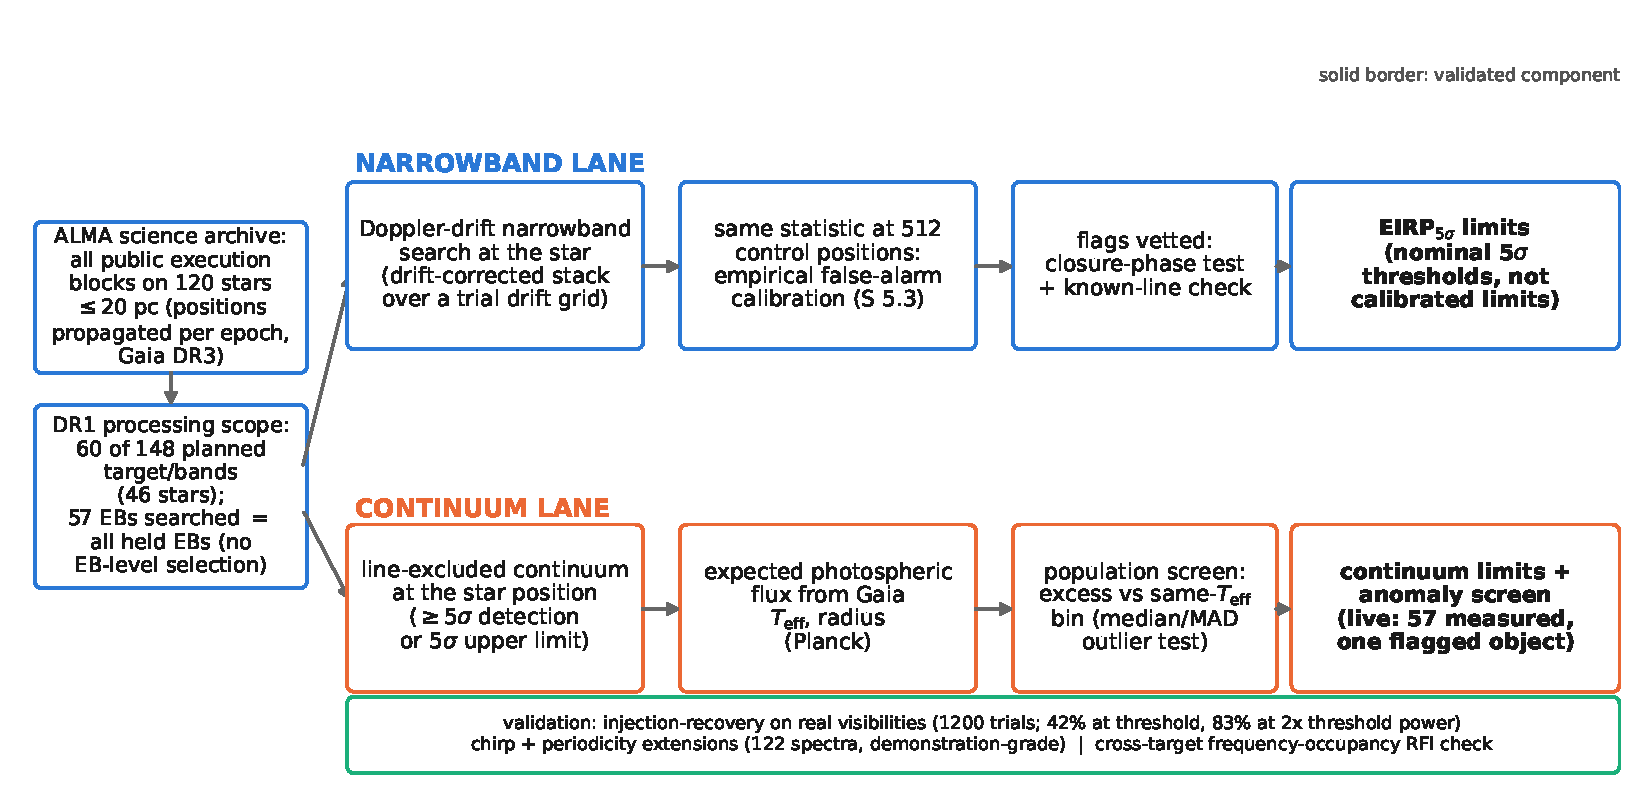
\includegraphics[width=\textwidth]{figures/pipeline_schematic.pdf}
\caption{Design of the survey. All public execution blocks on the 120
targets are mined from the ALMA science archive, with positions
propagated to each epoch from Gaia~DR3, and searched along two
independent lanes. The narrowband lane runs a Doppler-drift-corrected
narrowband search at the star position, calibrates its false-alarm rate
empirically against 512 control positions per window, and vets any
candidate with a closure-phase point-source test and a known-line
check, yielding per-window EIRP$_{5\sigma}$ limits. The continuum lane
measures the line-excluded continuum flux at the star position and
screens for anomalies against a same-$T_{\rm eff}$ comparison
population (Appendix~\ref{app:continuum}). Solid borders mark validated
components. The validation rail summarises the injection-recovery
(1200 trials, Appendix~\ref{app:inject}), chirp/periodicity, and
frequency-occupancy analyses.}
\label{fig:pipeline}
\end{figure*}

Three terms are defined here in strict nesting. A \emph{threshold
crossing} (internally, a ``hit'') is a single frequency and
drift-rate cell at the star's position whose statistic crosses the
nominal $5\sigma$ threshold. A \emph{candidate} is a window in which
a threshold crossing also passes the spatial-coincidence test against
that window's 512-position control ring. A \emph{vetted candidate}
survives every subsequent vetting stage (line check, closure phase,
cross-target occupancy, and human review) -- a status no object of
this release attains.

Stellar positions are propagated to each observation's epoch using
Gaia~DR3 proper motions and parallaxes. The searched drift-rate range
is the larger of (a) a generic frequency-scaled default
(12--13\,Hz\,s$^{-1}$\,GHz$^{-1}$), the literature fiducial of
\citet{Mason2024} with a threefold safety margin -- a design
boundary, not a claim that faster drift is physically implausible --
and (b) where the target hosts confirmed exoplanets, the maximum
line-of-sight orbital acceleration of the innermost known planet, so
a transmitter co-located with a short-period planet cannot drift out
of the searched window. For scale, $\dot\nu$ at frequency $\nu$
corresponds to a line-of-sight acceleration $a_{\rm los} =
c\dot\nu/\nu \approx 3.9$\,m\,s$^{-2}$ (${\sim}0.04$\,au around a
solar-type star); Earth-motion contributions
($\lesssim0.13$\,Hz\,s$^{-1}$\,GHz$^{-1}$ combined) are two orders of
magnitude below it and subsumed by the grid. These are
\emph{apparent} topocentric drift rates, including any deliberate
transmitted chirp as well as acceleration-induced drift, which the
survey does not attempt to distinguish -- the constraints of this
paper concern linear apparent drift within the searched range only.

Across the 225 windows the maximum searched drift rates span
1.1--5.9\,kHz\,s$^{-1}$, the native channel widths 15.3\,kHz to
31.25\,MHz (median 15.625\,MHz; the per-target file (Appendix~\ref{app:table})), and the trial
drift rates per window 2 to 1944 (median 4). The threefold margin is
consequential: at $1\times$ the release would have been blind to two
of its eight threshold-crossing windows, including the AU~Mic
candidate; at $5\times$ no disposition changes -- so transmitters
drifting faster than
${\sim}13$\,Hz\,s$^{-1}$\,GHz$^{-1}$ remain unconstrained.
Intra-integration smearing is negligible almost everywhere: at most
1.10 channels, median 0.001; only three windows have
$\eta_{\rm smear} < 0.99$ (marked $^{\ast}$ in the per-target file (Appendix~\ref{app:table});
Table~\ref{tab:smear}, Appendix~\ref{app:conventions}), the worst
being the $\beta$~Pic Band~6 fine window (effective threshold
1.74$\times$ nominal). The channel widths are the effective
resolutions (verified against the measurement sets' own spectral
window tables; Appendix~\ref{app:conventions}).

\subsection{Frequency and velocity reference frames}
\label{sec:frames}

Every frequency axis in this paper -- searched spectra, tabulated
ranges, candidate frequencies -- is \emph{topocentric}: the
frequencies delivered by the ALMA correlator, with no velocity-frame
shift applied to any data product at any stage. Velocities enter at
one place only, the stellar-frame line-exclusion mask of the vetting
stage, whose residual error is the catalogue radial-velocity
uncertainty alone; the conversion chain is given in
Appendix~\ref{app:conventions}. The stacking behind the search
statistic is coherent in frequency and in the drift-rate trial but
preserves no electric-field phase coherence between integrations.

The native channel width is also the linewidth convention under which
every EIRP threshold must be read, stated here because it is the
commonest source of confusion in comparing technosignature limits
across surveys: the detection statistic is the flux density in a
single channel after drift correction, so the quoted EIRP$_{5\sigma}$
applies to \emph{any} transmitter narrower than the native channel,
flat in the assumed linewidth, while dividing it by the channel width
gives the minimum detectable spectral power for wider transmitters.
Channelisation is the dominant price the archive exacts: the deepest
window (UV~Ceti Band~3, EIRP$_{5\sigma}=1.6\times10^{13}$\,W at
15.625\,MHz) would reach $4\times10^{9}$\,W had the same observation
been channelised at 1\,Hz ($P_{\min}\propto\sqrt{\Delta\nu}$, a factor
${\sim}4000$). The worked example, the sub-channel qualifications, the
smearing table, and the channel-width verification are in
Appendix~\ref{app:conventions} (Fig.~\ref{fig:linewidth}).

The narrowband search covers every distinct spectral window
configured for an observation, up to a cap of 8 windows per target to
bound compute cost. The cap bound exactly one target/band (61~Vir
Band~7: four of eight windows searched; the per-target file (Appendix~\ref{app:table})), so the
frequency-space selection function it introduces is fully tabulated
rather than hidden. Of the 60 target/bands, 53 have every configured
window searched; the remaining 3 ($\tau$~Cet, Kapteyn's Star,
Van~Maanen's Star) are represented by their deepest single window,
marked in the per-target file (Appendix~\ref{app:table}), with full multi-window coverage
deferred to the next release. Each searched window yields its own
EIRP$_{5\sigma}$ limit as a separate row of the per-target file (Appendix~\ref{app:table});
Figure~\ref{fig:eirp} plots only the deepest result per target/band.

Any threshold crossing is cross-checked against the rest frequencies
of the eight common mm/submm molecular species (\S\ref{sec:method},
Appendix~\ref{app:linecat}) using a $\pm50$\,km\,s$^{-1}$
stellar-frame mask -- velocity coincidence, not drift, being the
operative discriminant, since circumstellar emission sits at rest
offset by the gas's own kinematics whereas a technosignature is free
to appear at any frequency and drift rate. The searches as executed
used a narrower one-channel-width implementation that agrees with the
velocity-space form on every disposition here; the tolerance's
justification and the bandwidth it removes are in
\S\ref{sec:technosearch}.

Both the narrowband thresholds and the continuum fluxes are corrected
for ALMA's primary-beam response at the star's offset from the phase
centre. For most targets the correction is negligible (median factor
1.0001, 90th percentile 1.012, none above 2\%). Two datasets sit at
large offset -- Sirius~B (corrections 3.6--16\% across bands) and
$\epsilon$\,Eri Band~6 (2.9--3.4$\times$) -- where the Gaussian beam
form is itself an approximation; both are marked provisional in
the per-target file (Appendix~\ref{app:table}) and excluded from the headline ensemble
statistics. Excluding them changes neither endpoint of the quoted
EIRP range nor the median ($2.6\to2.9\times10^{14}$\,W) nor any
conclusion; recomputation against the holography beam model is
committed for the corrected tagged release.
\subsection{Reference transmitter benchmarks}
\label{sec:benchmarks}

For physical context the EIRP thresholds of \S\ref{sec:results} are
compared throughout to two human-transmitter benchmarks, both from
\citet{EarthDetectingEarth2025}: an Arecibo-like planetary radar
(S-band EIRP $2\times10^{13}$\,W -- the most powerful deliberate
directed transmitter an Earth-equivalent civilisation could point at
us, used purely as a technological-power benchmark and not as a claim
that such a radar radiates at mm/submm frequencies), and unintentional
Earth mobile-network leakage with no signalling intent (EIRP of order
$4\times10^{9}$\,W).

\subsection{Ancillary and validation analyses}
\label{sec:ancillary}

Four analyses beyond the narrowband search are executed in this
release, each specified in full online and summarised here only so far
as the main text depends on it; Table~\ref{tab:supp} (online) records
what each was applied to, its validation status, and whether it enters
the headline limits.

\emph{Injection-recovery validation} (Appendix~\ref{app:inject}).
Synthetic narrowband tones of known amplitude were injected into real
calibrated visibility data and recovered with the unmodified pipeline
(1200 trials across six window configurations, three bands, and both
resolution classes). Two outcomes carry into the limits. First, the
pipeline's per-channel time-median subtraction absorbs any
phase-steady carrier dwelling in one channel for more than roughly 40
per cent of the track; on coarse (15.625\,MHz) windows every in-grid
drift is sub-channel over the track, so this is total (0 of 500
coarse injections recovered from $4\sigma$ to $10\sigma$) and the
coarse-window limits bound transmitters time-variable on track
timescales rather than phase-steady carriers. Second, for the
drifting class on the fine window recovery is 17, 42, 58, 75 and 83
per cent at $4$, $5$, $6$, $8$ and $10\sigma$, giving
EIRP$_{50}=1.10\,$EIRP$_{5\sigma}$ and, as a bound,
EIRP$_{90}>2.0\,$EIRP$_{5\sigma}$ (Fig.~\ref{fig:completeness},
Table~\ref{tab:classcomp}). Every table here stays in nominal
EIRP$_{5\sigma}$; the occurrence limit of \S\ref{sec:discussion} is
the one place the measured completeness is folded in numerically, and
Band~8 completeness is transferred by shared construction rather than
measured.

\emph{Drift-ceiling caveat.} The searched ceiling is a fixed
$12$\,Hz\,s$^{-1}$\,GHz$^{-1}$, i.e.\ a line-of-sight acceleration
$|a| = 3.6$\,m\,s$^{-2}$, uniform across every window. This clears
Earth-rotation and Earth-orbit drifts by about two orders of
magnitude, but it sits $11$ per cent \emph{below} the
$4.0$\,m\,s$^{-2}$ appropriate to a close-in planet on a
TRAPPIST-1\,b-like orbit. Carriers on the most rapidly accelerating
bodies are therefore not fully covered, and the limits of
\S\ref{sec:discussion} are conditional on that ceiling
(Figure~\ref{fig:accel}).

\emph{Closure-phase vetting} (Appendix~\ref{app:closure}).
Threshold-crossing candidates face an automated test that single-dish
and beamformed surveys lack, since it requires multiple independent
baselines: the closure phase is exactly zero for an unresolved point
source at any sky position and immune to per-station calibration
errors, so inconsistency with zero at the drift-tracked candidate
frequency is evidence against celestial point-source behaviour. The
converse does not hold, which makes this a strictly one-sided
exclusion diagnostic and never an authentication. It is implemented
and simulation-validated but sensitivity-limited at this survey's flux
densities -- per-baseline S/N never exceeds 5.1 in the positive-control
fields -- so it can neither authenticate nor exclude any continuum
detection of this release. The three candidates are all consistent
with a point source ($z=0.16$ for AU~Mic; \S\ref{sec:technosearch}).

\emph{Population-level continuum anomaly screen}
(Appendix~\ref{app:continuum}). Because the sample is a census rather
than an interest-selected list, it supports an ancillary screen for
continuum flux anomalous relative to a star's own photospheric
expectation and to same-$T_{\rm eff}$ comparison stars. It is
exploratory, not a headline constraint: the samples are small (57
measurements: 17 detections, 40 limits; bins of 4--7 stars) and a
millimetre excess is at best an indirect, model-dependent observable
of waste-heat technology. Its outcome is one outlier, $\chi^1$~Ori at
Band~3 (excess ratio 2.52; resampled tail probability 0.53 in its
six-star bin -- the ranked outlier of a small sample), consistent
with astrophysical channels, on which no technosignature disposition
rests.

\emph{Extended and cross-target screens}
(Appendices~\ref{app:extended} and \ref{app:freqoccupancy}). The
primary search stacks at constant linear drift rate, so a chirped
(quadratic-drift) extension and a per-channel periodicity search were
run against the 122 retained spectra as a demonstration rather than a
survey-grade screen; their null behaviour is as expected
(star-exceeds-ensemble rates 10.7 and 13.1 per cent against an
11-per-cent chance rate), no instance is a candidate, and no limit
derives from them. Separately, this
single-pointing archival survey has no ON/OFF cadence for rejecting
radio-frequency interference, so its analogous resource is the many
unrelated stars sharing similar correlator setups: threshold crossings
towards different targets were cross-matched for recurrence at the
same observed sky frequency. Of the 366 star pairs whose searched
frequency ranges overlap, none falls within the matching kernel, with
one bookkeeping caveat -- the retained products cap each window's list
at 50 crossings, leaving 64 crossings of one $\beta$~Pic window
untested -- recorded with the kernel and coordinate caveats in the
appendix.
\section{Results}
\label{sec:results}

The counting quantities of this release -- systems, stars,
star/bands, windows, execution blocks, and projects -- are those of
Table~\ref{tab:searchspace} (\S\ref{sec:sample}); these levels are
not independent statistical trials, since unresolved binaries share
one measurement set.

The detailed results below report the $\le$20\,pc release of version
3.24 (see Scope of this version). Of the 148 target/bands planned for
that subsample (46 unique stars), 60 were searched to completion and
yielded a valid result; all values here correspond to the frozen
pipeline and data snapshot of this paper. The survey is strictly
volume-ordered (nearest star first; \S\ref{sec:sample}), so these
results are weighted towards the very nearest stars, spanning
1.3--19.6\,pc. Full per-target values, including each band's exact
searched frequency range, are given in the per-target file (Appendix~\ref{app:table})
(online-only Appendix~\ref{app:table}).

\subsection{Per-star summary}
\label{sec:starsummary}

Table~\ref{tab:starsummary} (online-only) gives the one-line-per-star
view complementing the per-window per-target file
(Appendix~\ref{app:table}): each star's deepest nominal
EIRP$_{5\sigma}$ threshold, its band, that band's continuum-lane
result, and the bands with searched windows. Two stars of the release
are continuum-only. All values are read directly from the per-target
file and add no new numbers; EIRP values are nominal native-channel
thresholds under the boxed rule of \S\ref{sec:method}, and continuum
fluxes are primary-beam corrected.


\subsection{Barnard's Star and Wolf~359}
\label{sec:barnardswolf}

Barnard's Star and Wolf~359 -- the second- and fourth-nearest stellar
systems -- have not, to our knowledge, previously been searched for
technosignatures at ALMA frequencies. Both yield non-detections from
public Band~6 archival data: EIRP$_{5\sigma}$ limits of
$6.15$--$6.89\times10^{13}$\,W (Barnard's Star, 4 windows) and
$7.84$--$9.10\times10^{13}$\,W (Wolf~359), with continuum upper limits
of 0.575 and 0.453\,mJy. These are the first reported mm-wave
constraints on either star.

\subsection{Data-quality exclusions and open items}
\label{sec:exclusions}

Status of the 148 target/bands planned for the $\le$20\,pc release:
60 searched to completion and reported here; two attempted and failed
at the process level, excluded from all counts; 86 queued for later
releases. Four classes of entry within the 60
are absent from the released per-target file
(Appendix~\ref{app:table}) and are itemised with their forensics in
Appendix~\ref{app:exclusions}: (i) four process-level search failures,
each still carrying a continuum non-detection and no EIRP threshold;
(ii) one pair excluded for data quality; (iii) windows partially
withheld for a noise-handling defect; and (iv) one relabelled entry,
with no measured value changing.

Item (iii) sets this paper's headline depth and is therefore stated
here. A reproducible defect produces implausibly small noise in a
minority of coarse-channel windows. Through version 3.25 it was
carried as a two-window exclusion named after the affected stars;
extending the sample beyond 20\,pc showed that a name-based exclusion
does not generalise, so it is now caught by a physical test. For a
correctly weighted measurement the product
$\sigma\sqrt{t_{\rm on}\,\Delta\nu_{\rm ch}}$ is set by system
temperature and collecting area, so it varies by factors of a few
across a heterogeneous archive; windows falling more than $100\times$
below the sample median are excluded. Six of 448 windows fail, across
five stars, separated from the rest of the sample by a factor
$1.5\times10^{3}$ in that product, so the threshold is not
fine-tuned. Their nominal thresholds, $2.0$--$7.8\times10^{12}$\,W,
would otherwise have set this paper's headline depth; excluding them,
the best threshold is $1.6\times10^{13}$\,W. The affected windows are
excluded, the combined continuum withheld, and each star's other
windows retained. The supporting audit is otherwise clean across all
225 windows except the four $\chi^{1}$~Ori Band~3 windows (elevated
system temperature; limits weakened, not invalidated), and all 120
census identifiers re-resolve through SIMBAD and \emph{Gaia} to 120
distinct sources inside 20\,pc.

\subsection{Technosignature search}
\label{sec:technosearch}

Fifty-six of the 60 target/bands yielded at least one narrowband
result (the four failures are itemised in \S\ref{sec:exclusions}),
spanning 225 spectral-window measurements after removal of 13
duplicate rows found in the catalogue audit
(Appendix~\ref{app:table}). The EIRP$_{5\sigma}$ limits span
$1.6\times10^{13}$--$7.1\times10^{16}$\,W, median
$2.7\times10^{14}$\,W (Figures~\ref{fig:eirp}, \ref{fig:coverage} and
\ref{fig:context}). As expected for a volume-ordered survey, the
deepest limits are for the nearest systems ($1.6\times10^{13}$\,W for
the UV~Ceti pair at 2.7\,pc); the shallowest is $\eta$~Corvi, the
first Band~8 target searched, where distance, coarse channels, and
receiver performance set the survey's current ceiling. Against the
benchmarks of \S\ref{sec:benchmarks}, only targets within
$\sim$3\,pc reach below the Arecibo-like planetary-radar EIRP, and
none approaches the $\sim4\times10^{9}$\,W of unintentional Earth
leakage -- a sobering calibration of what even a deep archival
mm-wave search cannot yet see.

Three narrowband features have been promoted to \emph{candidates}, in
the vocabulary defined after Figure~\ref{fig:pipeline}.
Table~\ref{tab:funnel} follows the decision cascade;
Table~\ref{tab:candidates} gives each candidate's disposition and the
test that decided it.

\begin{table}
\centering
\small
\caption{The narrowband decision cascade of this release, from trials
to disposition.}
\label{tab:funnel}
\begin{tabular}{@{}lr@{}}
\hline
Stage & Count \\
\hline
Channel $\times$ drift trial cells (all windows) & $1.97\times10^{7}$ \\
Control positions compared per cell-set & 512 per window \\
Threshold-crossing frequencies ($\geq5\sigma$ at star position) & 171 true / 107 tabulated$^{\rm a}$ \\
Windows containing $\geq$1 threshold crossing & 8 (5 stars) \\
Candidates (crossing $+$ star beats ring) & 3 (2 stars) \\
\quad dispositioned as circumstellar CO & 2 ($\beta$~Pic) \\
\quad consistent with empirical background & 1 (AU~Mic) \\
Vetted candidates (credible technosignatures) & 0 \\
\hline
\end{tabular}
\parbox{\columnwidth}{\footnotesize $^{\rm a}$The retained products cap
each window's crossing list at 50; the deficit is one window
(Appendix~\ref{app:freqoccupancy}).}
\end{table}

\begin{table}
\centering
\small
\setlength{\tabcolsep}{4pt}
\caption{The three candidates of this release and the test that
dispositioned each. `Line' is the stellar-frame offset from the
nearest catalogued transition (Table~\ref{tab:bpicaudit}); `Spatial /
recurrence' the star-versus-control outcome and, where one exists,
the same-star second-epoch test. No disposition rests on a single
test.}
\label{tab:candidates}
\begin{tabular}{@{}lllll@{}}
\toprule
Candidate & Band & Line & Spatial / recurrence & Disposition \\
\midrule
$\beta$~Pic & B3 & CO($1{\to}0$), $-2.7$\,km\,s$^{-1}$ & CO-consistent kinematics at 3 epochs, 2 transitions & circumstellar CO \\
$\beta$~Pic & B6 & CO($2{\to}1$), $-3.5$\,km\,s$^{-1}$ & as above (same gas component) & circumstellar CO \\
AU~Mic & B6 & none ($+379$\,km\,s$^{-1}$) & $T_\star=4.93$ vs ring max 7.70; no recurrence & empirical background \\
\bottomrule
\end{tabular}
\end{table}

Two questions are kept separate: is a release containing three
candidates more than this survey's own calibration predicts (a
counting question), and is any individual candidate statistically
distinguishable from the empirical background (answered in the
dispositions below)?

\subsubsection*{Survey-level false-alarm calibration}

Each window-level test compares the peak signal-to-noise ratio at the
star's position with the same statistic at 512 control positions --
an empirical calibration absorbing the per-window trials factor, since
the drift-rate grid and the thousands of channels are applied
identically to star and controls. From this version the statistic is
\emph{symmetric}: the on-source quantity is the single propagated
stellar position, exactly what each control contributes. Earlier
versions maximised it over a small region centred on that position
while each control remained a single position, and that asymmetry was
not benign: under a pure-noise null with exchangeable positions, the
maximum of $n_{\rm src}$ source-region positions exceeds that of
$n_{\rm ctrl}$ single controls with probability
$n_{\rm src}/(n_{\rm src}+n_{\rm ctrl})$, which for the
$n_{\rm src}=135$ region and 512 controls of a representative window
is 21 per cent -- and the measured region-max star-beats-ring rate,
67 of 448 windows (15.0 per cent), is of that order. The symmetric
statistic instead gives star-beats-ring in 6 of 448 windows (1.3 per
cent), consistent with the exchangeable expectation $1/513=0.19$ per
cent per window inflated by the real maps' heavy tails, and stable
against the 1.3 per cent measured on the $\le$20\,pc subsample alone.
It makes the nominal exchangeability rate the operative one, so the
survey-level false-alarm expectation follows directly rather than
through the bookkeeping ladder the asymmetry previously required.

A candidate is gated by the joint criterion, whose threshold leg
dominates the rate: only 22 of 448 windows contain any $\geq5\sigma$
crossing at the stellar position. Each window contributes at most the
exchangeable rate $1/(1+n_{\rm ctrl})=1/513$, so the pure-noise null
predicts $448/513=0.87$ flags across 448 windows. Four flagged
target/bands against 0.87 is not a significant excess, and three
carry independent astrophysical attributions (below), leaving one
marginal crossing -- the order of the expectation. This is the
operative survey-level false-alarm estimate; it absorbs
execution-block systematics into the fixed block margins and assumes
only that, within a block, crossing status is exchangeable with
star-beats-ring status -- the no-association null of interest.
Secondary bookkeeping models span 1.0--9.2 per cent
(Appendix~\ref{app:falsealarm}); the dominant residual uncertainty is
the star-beats-ring rate itself (Wilson 95 per cent interval
9.5--18.4 per cent), giving a 4--19 per cent bracket on $P(F\geq3)$.
One ensemble limit: with 512 controls the smallest resolvable
per-window $p$-value is $1/513$, so a Bonferroni threshold over 448
windows ($1.1\times10^{-4}$) lies below what the controls can
measure. They can show a crossing to be unremarkable but cannot
certify one as significant survey-wide; that burden falls on
localisation, recurrence, and astrophysical attribution, which decide
each flag below. The two $\beta$~Pictoris dispositions do not depend
on the bracket (they rest on kinematic attribution to a mapped disc),
the AU~Mic candidate's standing is a rank statement (invariant to the
bookkeeping model; conditional probability 41 per cent empirical, 34
per cent idealised), and no model in the bracket promotes any of the
three to a vetted candidate: no conclusion of this paper inverts
within the bracket.

The chance-crossing expectation is consistent with the raw trials
count once channel adjacency is handled, the star-beats-ring rate is
not driven by any single band, channelisation, or primary-beam-offset
stratum, and the control ring's geometry introduces neither a
primary-beam-gradient bias nor an inflated spatial trials factor;
these three robustness checks are reported in
Appendix~\ref{app:falsealarm}.

\subsubsection*{The symmetric star-versus-control null}

The survey's designed principal test applies the identical
source-region, drift-rate, and frequency maximisation at the star's
position and at every one of the 512 control locations under a single
search rule. The identical-treatment requirement cannot be met from
the frozen release products, so its domain is the seven locally
reprocessed windows -- the six validation windows and the AU~Mic
candidate's first-epoch block -- all of which give $T_\star=3.7$--$4.9$
against control maxima of 6.7--7.7, $p=0.81$--1.00
(Figure~\ref{fig:symcdf}, online-only appendix): the star position is
statistically exchangeable with its control ring wherever the test
can be run at full symmetry, and no window shows star-side excess.
Extending it to all 225 windows requires per-window raw-visibility
reprocessing that the retained products do not support, so until the
remaining measurement sets are re-run the empirical
star-versus-ring calibration above remains the operative release-wide
estimate, with the symmetric statistic a validation subset; the machinery ships with the release,
and the full statement, together with the consolidated family-wise
trials factors of Table~\ref{tab:trials}, is in
Appendix~\ref{app:falsealarm}.

\subsubsection*{The $\beta$~Pictoris candidates: circumstellar CO}

The first two candidates are both towards $\beta$~Pictoris, a
debris-disc system with previously reported CO emission
\citep{Matra2017}: one in Band~3 at 115.2606\,GHz, 10.56\,MHz below
the CO($J{=}1{\to}0$) rest frequency, the other in Band~6 at
230.5161\,GHz, 21.87\,MHz below CO($J{=}2{\to}1$). Neither
coincidence is exact, so the automated line check did not catch them.
Carried through the full frame chain (Table~\ref{tab:bpicaudit};
Fig.~\ref{fig:bpicvel}), the offsets correspond to the same kinematic
component -- $-2.7$ and $-3.5$\,km\,s$^{-1}$ from stellar systemic,
0.74\,km\,s$^{-1}$ apart -- in the two lowest CO rotational
transitions of a system with directly detected circumstellar CO; the
coarse Band~6 window without a candidate, from a third epoch six
years earlier, independently shows CO at $-3.6$\,km\,s$^{-1}$ in the
same frame. All three epochs and both transitions land within
$0.9$\,km\,s$^{-1}$ of each other and $3.6$\,km\,s$^{-1}$ of
systemic, deep inside the $\pm50$\,km\,s$^{-1}$ mask. The raw
topocentric offsets ($-27.5$ and $-28.4$\,km\,s$^{-1}$) become these
stellar-frame values only after the barycentric correction and the
catalogued systemic velocity are applied -- the frame chain matters.
We attribute both candidates to line contamination from this
kinematically offset CO emission.

Their empirical significance under the release background is
nonetheless extreme, so the attribution should not be mistaken for
dismissal: the Band~3 region peak of 20.3 exceeds all 225 per-window
control maxima (add-one $p<0.0044$), and the Band~6 peak of 12.8
exceeds all but one -- that window's own CO-filled control ring,
which reaches 15.2 (by far the highest control maximum of the
release; $p\approx0.0088$). Standing out this sharply is why they
demanded astrophysical attribution rather than summary rejection as
noise. The attribution came from subsequent inspection of the offsets
against known CO kinematics, not from the automated chain (the
one-channel line check tolerated their offsets; closure phase, which
they pass, does not discriminate line emission from an artificial
point source); the alternative would require a transmitter placed
coincidentally at matched offsets from two CO transitions in the same
star.

\begin{figure}

\includegraphics[width=\columnwidth]{figures/bpic_velocity_space.pdf}
\caption{Stellar-frame velocity offsets of the candidate windows,
carried through the full frame chain (topocentric $\rightarrow$
barycentric $\rightarrow$ stellar; Table~\ref{tab:bpicaudit}).
Shaded band: the $\pm50$\,km\,s$^{-1}$ molecular-line exclusion mask.
\emph{Top:} the two $\beta$~Pictoris candidates fall well inside the
mask as a single kinematic component within $3.5$\,km\,s$^{-1}$ of
stellar systemic, matching the resolved, previously mapped disc
\citep{Matra2017}; the inset resolves the pair (0.7\,km\,s$^{-1}$
apart). \emph{Bottom:} the AU~Mic candidate sits at
$+379$\,km\,s$^{-1}$ in the stellar frame, far outside any
circumstellar tolerance; it is dispositioned by its spatial and
recurrence behaviour, not by the mask.}
\label{fig:bpicvel}
\end{figure}

\begin{table*}
\centering
\small
\caption{Line-attribution audit of the three candidate windows
(first three rows) and the coarse $\beta$~Pictoris Band~6 window
without a candidate
that independently shows the same CO component, carried through the
frame chain of \S\ref{sec:frames}. Topocentric offsets are observed
minus catalogued rest frequency (CO $J{=}1{\to}0$ 115.271202\,GHz,
CO $J{=}2{\to}1$ 230.538000\,GHz, \citealt{Pickett1998}). The
barycentric correction is the Earth-ephemeris term at the
execution-block mid-time (block uids in Table~\ref{tab:ebs}); the
systemic radial velocities are the catalogued values (SIMBAD;
\emph{Gaia} DR3 for $\beta$~Pictoris, \citealt{GaiaDR3}; \emph{Gaia}
DR2 for AU~Mic, \citealt{Fouque2018}).}
\label{tab:bpicaudit}
\begin{tabular}{@{}llrrrrrr@{}}
\toprule
Flag & UTC start & $f_{\rm obs}$ (GHz) &
Transition & Topo.\ offset & Bary.\ corr. & $v_{\rm sys}$ &
Stellar-frame \\
 & & & & (MHz; km\,s$^{-1}$) & (km\,s$^{-1}$) & (km\,s$^{-1}$) &
offset (km\,s$^{-1}$) \\
\midrule
$\beta$~Pic B3 & 2022-03-02 23:14 & 115.260644 &
CO($1{\to}0$) & $-10.56$; $-27.46$ & $-7.90$ & $+16.84$ & $-2.72$ \\
$\beta$~Pic B6 & 2019-03-12 00:14 & 230.516128 &
CO($2{\to}1$) & $-21.87$; $-28.44$ & $-8.15$ & $+16.84$ & $-3.45$ \\
AU~Mic B6 & 2014-08-18 04:01 & 230.825230 &
CO($2{\to}1$) & $+287.23$; $+373.51$ & $-10.02$ & $-4.71$ & $+378.82$ \\
$\beta$~Pic B6$^{\dagger}$ & 2013-10-06 06:23 & 230.528134 &
CO($2{\to}1$) & $-9.87$; $-12.83$ & $+7.63$ & $+16.84$ & $-3.62$ \\
\bottomrule
\end{tabular}
\parbox{\textwidth}{\footnotesize $^{\dagger}$Coarse
Band~6 window without a candidate (the per-target file (Appendix~\ref{app:table})); shown
because it independently exhibits the same CO component as the
candidate fine window of the same band.}
\end{table*}

\subsubsection*{Line exclusion: definition, cost, and limits}

The searches ran with an automated line check matching a crossing
against catalogued rest frequencies within one spectral channel at
zero drift. The $\beta$~Pictoris candidates showed that check
inadequate: both fell outside its one-channel tolerance (by 10.6 and
21.9\,MHz) while corresponding, after the frame chain, to a kinematic
component within 3.6\,km\,s$^{-1}$ of stellar systemic of a resolved,
previously mapped disc -- exactly the regime a channel-width tolerance
is blind to. Before publication every crossing was reclassified with a
velocity-space mask ($\pm50$\,km\,s$^{-1}$ in the stellar frame around
each catalogued transition), which is the published pipeline's
line-exclusion definition from this release onward. Its kinematic
justification, its empirical conservatism, the retrospective
reclassification of every crossing, and the ``Schelling point''
counter-argument that a deliberate communicator might choose exactly
these frequencies are set out in Appendix~\ref{app:linemask}; applied
retrospectively the mask rejects exactly the two $\beta$~Pictoris
candidates and changes no other disposition, and of the 106 unique
tabulated candidate frequencies across the ten crossing windows 101
are line-coincident within the mask and suppressed by the clean
search, whose product is the remaining five.


The masking cost is stated on one definition throughout: every JPL
catalogued transition of the eight species (276 transitions),
displaced by each system's radial velocity, $\pm50$\,km\,s$^{-1}$
stellar-frame half-width, intersected with each window and merged.
The release effectively searches 82.3\,GHz of unique sky frequency --
the disjoint union of the searched windows minus the part of the mask
inside it (Figure~\ref{fig:coverage}) -- down from 87.2\,GHz before
masking (a 5.7 per cent reduction). Summed over the 225 windows, the
mask removes 22.2\,GHz of the 378.9\,GHz of gross window-bandwidth
(5.9 per cent; per-species, per-band breakdown in
Table~\ref{tab:maskband}, online-only appendix); the per-window
usable fraction has median 0.960 (10th percentile 0.790). Union
bandwidth is exposure-blind -- a window visited for seconds counts
the same as one integrated for an hour -- so we also report
exposure-weighted quantities: the summed per-star frequency union is
371.9\,GHz (stars contribute overlapping sky frequency), and the
summed product of on-source time and searched bandwidth is
$8.3\times10^{5}$\,s\,GHz (per-window on-source time spans
12.1--5274\,s, median 2570\,s). The mask governs dispositions, not the
noise-derived thresholds, so the quoted EIRP$_{5\sigma}$ values are
unchanged; no signal was found outside the excluded molecular-line
velocity regions in any window. The mask is thus a selection effect
of the survey's design: no constraint is placed on transmitters
within the excluded regions -- 5.9 per cent of the searched bandwidth
-- and a search for deliberately line-adjacent carriers would need a
complementary strategy. The exposure is not limited to the candidate
windows: 131 of 225 windows (58 per cent) contain at least one
catalogued transition of the eight species in-band, and all eight
crossing windows do, yet in none does a crossing fall within one
native channel of a rest frequency -- precisely the regime the
velocity-space criterion covers.

\subsection{AU~Mic: reclassified, and why the criterion changed}
\label{sec:aumic}

The AU~Mic crossing in ALMA Band~6 at 230.83\,GHz was carried as a
candidate through version 3.24 and is \emph{not} a candidate under
the symmetric criterion adopted here. It is a single-epoch threshold
crossing statistically indistinguishable from the empirical control
population: 10 of its own 512 controls reach or exceed the stellar
statistic, an empirical $p=0.021$ nowhere near the $1/513$ floor the
criterion requires. It also fails two direct, pre-named tests -- it
is not localised at the stellar position, and it does not recur at a
second epoch (Table~\ref{tab:aumic}). It is the worked example that
motivated the change: under the old region-max statistic its
135-position source maximum (5.97) cleared the control maximum (5.85)
while the star itself (5.22) did not -- the asymmetry quantified in
\S\ref{sec:technosearch}.

\begin{table}
\centering
\small
\setlength{\tabcolsep}{4pt}
\caption{The AU~Mic candidate frequency (230.8252\,GHz) under the
three treatments that decide it: the release's frozen products
(region-max statistic), the fully symmetric reprocessing of the same
first-epoch execution block (2014 August~18; observatory calibration
recipe applied verbatim), and the second-epoch block of the same
programme (2014 June~5; identical search treatment).}
\label{tab:aumic}
\begin{tabular}{@{}lrrr@{}}
\toprule
 & Release & Symmetric & Second epoch \\
Statistic & (region-max) & reprocess. & (recurrence) \\
\midrule
Star statistic & 5.97 & 4.93 & 4.77 \\
Control maximum (512) & 5.85 & 7.70 & 6.78 \\
Star rank $p$ (add-one) & --- & 0.81 & 0.97 \\
Single-position star statistic & 5.22 & --- & --- \\
Per-channel S/N (zero drift) & --- & 2.46 & 2.22 \\
Peak drift (Hz\,s$^{-1}$) & 1418.5 & 1593 & 1281 \\
\bottomrule
\end{tabular}
\end{table}

The three tests that decide it are reported in full in
Appendix~\ref{app:aumic}. \emph{Localisation}: the first-epoch block,
reprocessed from the raw science data model with the observatory
pipeline's own recipe and searched with the symmetric statistic, gives
$T_\star=4.93$ against a control maximum of 7.70 ($p=0.81$) -- no
localised excess at the stellar position. \emph{Recurrence}: the one
further public Band~6 block covering 230.83\,GHz, at comparable band
rms, gives $T_\star=4.77$ against a control maximum of 6.78
($p=0.97$), a clean non-recurrence that rejects a continuous or
repeating source at this frequency and these epochs without
constraining intermittent transmission. \emph{Statistical scale}: the
on-source peak lies at the 94.7th percentile of the per-window
control-maxima distribution (add-one empirical $p=0.057$ before any
correction across 225 windows), the kind of marginal excess the rate
calculation predicts. The candidate coincides with no catalogued
molecular transition (287\,MHz from CO $J{=}2{\to}1$), and
closure-phase vetting finds it consistent with a point source --
one-sided evidence only (Appendix~\ref{app:closure}). Two pieces of
astrophysical context recorded there, neither the basis of the
rejection, are AU~Mic's flare activity -- which the candidate block's
own quiescent 0.15\,mJy continuum argues against -- and the debris
belt, whose smooth structure raises star and controls alike.

The archival epochs also bound what this release can say about duty
cycle: each star was observed in one to three execution blocks,
searched independently with no epoch stacking, so the non-detection
concerns the archival epochs observed, not permanent activity. The
proper-motion-matched archive census (\S\ref{sec:discussion}) counts
107 unique public on-star execution blocks over the 44 searched stars
against the 57 searched; that surplus is the recurrence pool the
second-epoch test drew on, and \S\ref{sec:discussion} turns the epoch
structure into an explicit duty-cycle constraint.
\subsection{Ancillary results}
\label{sec:ancillaryresults}

Three ancillary results are reported in full online.

\emph{Integration-time audit} (Appendix~\ref{app:audit}). The
on-source integrations quoted here were reconstructed from pipeline
bookkeeping rather than retained natively, so all 227 window-level
records were audited against the ALMA archive's own exposure
accounting: of the 58 star--execution-block groups, 53 are
conservative, three agree to better than 1 per cent, and two
over-count -- AT~Mic by a factor 1.43, an internally diagnostic
dump-bookkeeping artefact already corrected to the archive's 877\,s in
Table~\ref{tab:duty}, and CD$-$38~10980 by 7 per cent. No EIRP
threshold depends on the audited quantity, since thresholds derive
from the measured per-channel rms rather than from integration time;
the audit is conservative for every window of both candidate hosts, so
no disposition changes; and the exposure-weighted coverage figure of
\S\ref{sec:technosearch} is at worst optimistic by less than 1 per
cent. The defect class this audit caught was found by chance in one
target, which is why a direct per-execution-block export is committed
for the next release.

\emph{Continuum search} (Appendix~\ref{app:contsearch}). Of the 57
target/bands with a usable continuum measurement, seventeen show a
$\geq5\sigma$ detection and forty are non-detections
(Figure~\ref{fig:eirp}, right panel), the latter reaching upper limits
of 0.036--3.6\,mJy (median 0.52\,mJy), the deepest towards TRAPPIST-1
in Band~3. Every detection is astrophysically unsurprising: the
unresolved UV~Ceti binary, six young or active systems with known
debris discs or chromospheric activity, six showing the photospheric
flux expected for their spectral types, and two late-M dwarfs with
documented strong magnetic activity, of which the auroral emitter
LSR~J1835$+$3259 merits deeper follow-up. This lane is experimental:
its statistical power is unquantified at this depth and its link to
technology indirect and model-dependent, so no technosignature
disposition rests on it.

\emph{Serendipitous molecular-line catalogue}
(Appendix~\ref{app:linecat}). The line-exclusion step of the continuum
search identifies every $\geq5\sigma$ outlier channel as a byproduct,
and no existing mm/submm line survey of the solar neighbourhood is
drawn from a distance-limited census of archival coverage. Across the
subset scanned to date, 18 outlier channel groups were found: twelve
are single- or few-channel features with no known transition within
300\,MHz, most plausibly statistical; six are plausibly real --
CO($J{=}1{\to}0$) and CO($J{=}2{\to}1$) towards $\beta$~Pictoris, a
marginal two-epoch CO($J{=}2{\to}1$)-consistent feature towards
HD~285968, and a single-channel feature 195\,MHz from
SiO($J{=}5{\to}4$) towards HD~53143. All are reported openly,
including the two we consider probably spurious, and the
machine-readable catalogue ships with the tagged public release.
\begin{figure*}
\centering

\includegraphics[width=0.95\textwidth]{figures/eirp_continuum_vs_distance.pdf}
\caption{Nominal technosignature EIRP$_{5\sigma}$ thresholds (left;
every threshold drawn as a downward bar marking an upper limit) and
continuum flux
densities (right; downward triangles are $5\sigma$ upper limits, i.e.\
5$\times$ the map rms noise, with rms values given per target in
the per-target file (Appendix~\ref{app:table}); filled circles are
detections) as a function of distance, for the 60 target/bands (46
unique stars) of this release; the left panel shows one deepest EIRP
point per star for the 44 stars with completed narrowband searches
(two stars have continuum-only coverage), and
the right panel the 57 target/bands with usable continuum maps. The two
targets with candidate windows ($\beta$~Pictoris, Bands 3 and 6, and
AU~Mic, Band 6) are marked with stars; the $\beta$~Pictoris
candidates are identified in the text as CO disc emission, and the
AU~Mic candidate as a marginal excess not statistically distinguishable from the
empirical background distribution of this release, so neither is a
genuine technosignature. The left panel also
marks, as a reference line, the EIRP of an Arecibo-like planetary radar
($2\times10^{13}$\,W, the most powerful deliberate transmitter yet built
by humans; \citealt{EarthDetectingEarth2025}, \S\ref{sec:benchmarks}) --
a power comparison only, not a detectability claim at these wavelengths.
The ordinate begins at $5\times10^{12}$\,W; typical unintentional Earth
radio leakage ($\sim4\times10^{9}$\,W of total isotropically radiated
power rather than beamed EIRP) lies far below the plotted range and is
not shown. Plotted
EIRP$_{5\sigma}$ values are nominal 5$\sigma$ thresholds, to be read
under the boxed reading rule of \S\ref{sec:method}: the injection
campaign of Appendix~\ref{app:inject} measures ${\sim}42$\% recovery
at the threshold itself for morphology-matching carriers (${\sim}83$\%
at twice the threshold power), with phase-steady carriers on
coarse-channel windows suppressed by construction.}
\label{fig:eirp}
\end{figure*}



\begin{figure*}
\centering

\includegraphics[width=\textwidth]{figures/freq_coverage.pdf}
\caption{Frequency coverage of this release. (a) Number of searched
windows covering each frequency (0.01-GHz grid; the union is
87.2\,GHz in 36 disjoint intervals from 89.6 to 495.1\,GHz). (b) The
number of windows whose EIRP$_{5\sigma}$ threshold lies below the
labelled power as a function of frequency -- a sensitivity-weighted
version of the coverage panel, $N(<\mathrm{EIRP}_{5\sigma};\nu)$: 17,
59, 167, and 220 of the 225 windows lie below
$3\times10^{13}$, $10^{14}$, $10^{15}$, and $10^{16}$\,W respectively,
and none reaches below the survey floor of $1.6\times10^{13}$\,W.
As throughout this paper, thresholds are nominal 5$\sigma$ values with
the measured recovery carried separately
(Appendix~\ref{app:inject}).}
\label{fig:coverage}
\end{figure*}



\section{Discussion}
\label{sec:discussion}
This paper is the survey's first stand-alone processed release, and
its results are preliminary by construction: 60 of 148 planned
target/bands ($\sim$41 per cent) are complete, and the processed
subset is sensitivity-ranked -- nearest, most sensitively-constrained
systems first -- so it is not an unbiased draw, and the full sample
will extend these results to larger distances and shallower faint-end
limits. The citable results are the survey-level statements
(methodology, completeness calibration, benchmark comparisons); the
per-target values of the per-target file (Appendix~\ref{app:table}) are a snapshot that
specific rows will supersede. No credible technosignature has been
found: no signal matching the searched frequency, drift-rate,
temporal and spectral morphology was detected above the nominal
instrumental threshold during the analysed archival intervals, and
the quoted EIRP$_{5\sigma}$ thresholds of the per-target file (Appendix~\ref{app:table}) bound
any transmitter present above them. Two candidates towards $\beta$\,Pic are attributable to
CO disc emission -- underlining, as \citet{Mason2024} highlight, the
importance of checking any mm-band narrowband crossing against known
molecular transitions; that check is automated for every crossing
(\S\ref{sec:method}) and now uses a velocity-space match applied
retroactively to every window (\S\ref{sec:technosearch}). The third,
marginal candidate (AU~Mic, \S\ref{sec:aumic}) is not statistically
distinguishable from the empirical background and remains recorded
for future re-examination rather than dismissed.

The scale of the space searched -- the unique-frequency union
surviving the molecular-line velocity exclusion mask, its unmasked
counterpart, and the exposure-weighted on-source time--bandwidth
product -- is stated on one definition throughout in
\S\ref{sec:technosearch} and Figure~\ref{fig:coverage}. For context
on the drift ceiling, of the
37 planets known around the 15 planet-hosting targets only
TRAPPIST-1\,b, in its edge-on worst case at
$\sim$13\,Hz\,s$^{-1}$\,GHz$^{-1}$, reaches it; GJ~581\,e,
61~Vir\,b, and TRAPPIST-1\,c reach roughly half of it, and the
remaining 33 planets all sit well inside the searched
grid.\footnote{Star--planet relative accelerations $GM_\star/r^{2}$
from NASA Exoplanet Archive planetary-companion parameters (Mission
Star/Planet table, accessed 2026 September), maximised over orbital
phase and inclination.}

Table~\ref{tab:searchspace} consolidates the survey selection
function -- the axes along which a transmitter is or is not
detectable; Table~\ref{tab:bands} (online-only appendix) decomposes
the same release by ALMA band.

\begin{table}
\centering
\small
\setlength{\tabcolsep}{4pt}
\caption{The survey selection function of this release, consolidated.
All entries are counts or measurements of this release as frozen,
except the measured-recovery row, which is the injection campaign of
Appendix~\ref{app:inject}. The
EIRP$_{5\sigma}$ and flux-density rows are two forms of the same
thresholds: total power delivered within one native channel, and the
corresponding flux density (the two are related by
EIRP $= 4\pi d^{2} S_{\rm min} \Delta\nu_{\rm ch}$).}
\label{tab:searchspace}
\begin{tabular}{@{}l r@{}}
\hline
Quantity & Value \\
\hline
Census stars (catalogue entries; systems) & 120; 113 \\
Stars processed / with narrowband windows & 46; 44 (42 systems) \\
Target/band datasets & 60 of 148 planned (41\%) \\
Searched spectral windows (deduplicated) & 225 \\
Unique frequency union & 87.2\,GHz (36 intervals, 89.6--495.1\,GHz) \\
Effective after line-exclusion mask & 82.3\,GHz (5.7\% of the union masked) \\
Native channel widths & 15.3\,kHz -- 31.25\,MHz (median 15.625\,MHz) \\
Drift-rate ceilings & 1.1--5.9\,kHz\,s$^{-1}$ (12.0--13.3\,Hz\,s$^{-1}$\,GHz$^{-1}$) \\
Nominal flux-density thresholds $S_{\rm min}$ & 4.9\,$\mu$Jy -- 1.3\,Jy (median 7.3\,mJy) \\
Nominal EIRP$_{5\sigma}$ thresholds & $1.6\times10^{13}$--$7.1\times10^{16}$\,W (median $2.7\times10^{14}$) \\
Measured tone recovery (1200 trials, B3/B6/B7) & 0/500 static carriers (coarse, by construction); $42\%\rightarrow83\%$ for drifting carriers at $5\rightarrow10\sigma$ (fine; Fig.~\ref{fig:completeness}) \\
Star/bands with successful narrowband results & 56 \\
Star/bands with usable continuum measurements & 57 \\
Public on-star execution blocks available, all bands$^{c}$ & 107 \\
Window-level bookkeeping records (not EBs; ${\sim}4$ spw rows per pair) & 227 \\
Execution blocks; unique projects & 57; 36 \\
Observing epochs & 2013 Oct 6 -- 2025 Jun 11 \\
Per-star on-source integration & 1\,min -- 2.8\,h (median 46\,min) \\
Threshold crossings / windows with crossings / candidates & 107 / 8 / 3 \\
\hline
\end{tabular}
\par\vspace{3pt}
\parbox{\columnwidth}{\footnotesize $^{c}$From the proper-motion-matched
archive census of 2026 September~9 (\S\ref{sec:discussion}). Note.
Thresholds are nominal
5$\sigma$ instrumental values; the degree to which a drifting,
off-grid, or partially in-channel signal of a given amplitude is
actually recovered is a separate measured quantity, carried by the
injection campaign of Appendix~\ref{app:inject} rather than assumed
from the threshold.}
\end{table}


Coverage eligibility and search completeness are different quantities
and we keep them separate. The census of public usable ALMA data
(\S\ref{sec:sample}) establishes eligibility: 148 planned target/band
combinations within 20\,pc, of which the 60 processed here fall
within this release's scope; every held execution block was searched,
so no EB-level selection lies behind the 57. Availability is
measured directly rather than inherited from the release bookkeeping:
a proper-motion-matched census of the ALMA archive (2026
September~9; public rows, all bands, pointing within 30\,arcsec of
the propagated stellar position at the observation epoch) counts 107
unique public on-star EBs for the 44 searched stars, and re-finds 56
of the 57 searched EBs (the exception, TRAPPIST-1's Band~7 execution
A002/Xcccc19/X5564, is carried by \texttt{obscore} only through its
calibrator-field row -- an archive-representation artefact biasing
the census low by one for that star). The difference between
availability and scope -- further epochs of the same target/bands and
bands not processed here -- is the recurrence pool the AU~Mic
second-epoch test of \S\ref{sec:aumic} drew on. The full selection
funnel, from archive availability to the zero-candidate outcome, is
Figure~\ref{fig:selection} (online-only appendix), and the
machine-readable ledger \texttt{v323\_star\_coverage.json} gives
per-star distance, availability, scope, and searched frequency
intervals.

Figure~\ref{fig:accel} (online-only appendix) shows the drift ceiling
as an explicit selection function over planet period and host mass,
and its cost is stated plainly: a transmitter bound to any known
planet in the sample other than the innermost TRAPPIST-1 planets
would produce drift rates the search covers in full; one whose drift
exceeds the ceiling -- a closer-in or more massive companion than any
known here, or a rapidly manoeuvring platform -- is outside the
searched grid and sacrificed by design (Appendix~\ref{app:extended} recovers
some non-linear morphologies). The host-mass dependence is weak
($a \propto M_\star^{1/3}$ at fixed period), so the ceiling is
effectively a function of orbital period alone; and the calculation
constrains only transmitters co-located with \emph{known} planets --
one on an undiscovered planet, a free-flying platform, or any
structure with accelerations of its own choosing is covered only in
so far as its drift falls within the searched grid. A coverage
fraction along one axis of a multidimensional haystack (frequency,
drift rate, sensitivity, duty cycle, sky position) is not a haystack
volume, and we quote it as such.

Placing the release against the published haystack of
\citet{Wright2018} is likewise best done axis by axis. On their
frequency axis (10\,MHz--115\,GHz), only the Band~3 portion of our
union lies inside their boundaries (20.6\,GHz of 115\,GHz, or 0.18 of
the axis, and a part their Hz-resolution surveys reach far more
finely); the remaining 66.6\,GHz (Bands~4--8, 125--495\,GHz) lies
entirely outside it -- the genuinely new territory of this release.
On their transmitted-bandwidth axis (0--20\,MHz), a single-channel
search of native channels probes a fraction set by the channel width
(window-mean 0.63, median 0.78). On their sensitivity axis, our
median threshold ($7.3$\,mJy across a 15.625-MHz channel, i.e.\
$\phi\approx1.1\times10^{-21}$\,W\,m$^{-2}$) detects a $10^{13}$\,W
transmitter only within ${\sim}0.9$\,pc. Against the only prior
ALMA-archival technosignature search, \citet{Mason2024} reach 28
bycatch targets at $\geq$1.01\,kpc with a deepest quoted
EIRP$_{\rm min}$ of $6.91\times10^{17}$\,W, whereas this release's 42
systems all lie inside 20\,pc at median per-target thresholds
${\sim}2500\times$ deeper: the two searches occupy nearly disjoint
corners of the same haystack, near versus deep. We do not multiply
these fractions into a combined haystack coverage -- the axes are
strongly coupled (distance and sensitivity above all), and a product
of marginal fractions would misstate the true overlap by orders of
magnitude.

\subsection{Occurrence limits}

What a zero-detection result bounds is a fully conditioned quantity.
Writing the per-system completeness as
\begin{equation}
C_i(P) = F_i\,R_i(P)\,D_i\,C_{i,\rm drift},
\label{eq:conditioning}
\end{equation}
where $F_i$ is the probability that the transmitter's sky frequency
falls inside the spectral intervals actually searched for system $i$,
$R_i(P)$ the probability that a transmitter of EIRP $P$ would have
crossed system $i$'s detection threshold had it been emitting at that
frequency, $D_i$ the probability that it was emitting during the analysed
archival interval, and $C_{i,\rm drift}$ the recovery probability for
a carrier of the searched drift and temporal morphology
(Appendix~\ref{app:inject}), the probability of zero credible
detections when a fraction $f$ of systems hosts a matching
transmitter is
\begin{equation}
P(N_{\rm det}=0\,|\,f)=\prod_{i=1}^{N_{\rm sys}}\left(1-f\,C_i\right),
\label{eq:prevalence}
\end{equation}
and the one-sided 95\% upper limit $f_{95}$ solves
$P(N_{\rm det}=0\,|\,f_{95})=0.05$.

\noindent\fbox{\parbox{0.96\columnwidth}{\small
\emph{Reading rule.} Among the ALMA-observed systems, fewer than
$f_{95}(P)$ per cent host a transmitter of EIRP $\geq P$ that was
emitting during the archival observations, at a sky frequency within
the particular spectral intervals searched for that system, with drift
and temporal morphology lying within the searched class.}}

\noindent We evaluate Eq.~\ref{eq:prevalence} on the 42 independently
observed systems (44 narrowband-searched stars; the UV~Ceti and
AT~Mic binaries share observations and are counted once each) in two
forms (Table~\ref{tab:occurrence}). The \emph{thresholded} form is
the step function the retained products support directly: $R_i(P)=1$
when system $i$'s deepest window threshold lies below $P$ and 0
otherwise, $F_i=D_i=1$ by construction. The \emph{measured} form
integrates the injection-recovery curve of Appendix~\ref{app:inject}
over each system's searched bandwidth,
$R_i(P) = \sum_w \Delta\nu_w\, {\rm rec}(P/{\rm
EIRP}_{5\sigma,w}) / \sum_w \Delta\nu_w$, folding in the
$42\rightarrow83$ per cent threshold-to-$2\times$-threshold recovery
of the searched class (including the channel-phase dependence of
the placement-pooled curve). It covers the 24 systems with at
least one fine-channel window; the 18 coarse-channel-only systems
have no measured recovery for the drifting class (static carriers
there are suppressed by construction), so the measured ladder is a
24-system bound, not a 42-system one -- the thresholded ladder
remains the only survey-wide form at this depth. The Band~8 windows
share the coarse-channel construction and their completeness is
likewise transferred by shared construction, not measured
(Appendix~\ref{app:inject}).

\begin{table}
\centering
\small
\setlength{\tabcolsep}{4pt}
\caption{The 95 per cent upper limit $f_{95}(P)$ on the occurrence of
transmitters above EIRP $P$, in the two forms of the text. $n$ is the
number of systems with non-zero completeness at that $P$. The
measured form is defined on the 24 fine-channel systems (18
coarse-only systems have no measured recovery for the drifting
class); `vacuous' means no system has non-zero completeness, so no
bound exists.}
\label{tab:occurrence}
\begin{tabular}{@{}lrrr@{}}
\toprule
$P$ (W) & \multicolumn{2}{c}{$f_{95}$ thresholded} & $f_{95}$ measured \\
 & $n$ & limit & ($n$) \\
\midrule
$3\times10^{13}$ & 4 & 52.7\% & vacuous (2) \\
$10^{14}$ & 17 & 16.2\% & 98.8\% (11) \\
$10^{15}$ & 39 & 7.4\% & 51.9\% (22) \\
$10^{16}$ & 42 & 6.9\% & 44.5\% (24) \\
\bottomrule
\end{tabular}
\end{table}

Three caveats bound how far these numbers can be pushed. First, even
the measured form fixes $F_i=D_i=1$ and the per-system recovery at
the configuration level: it is a frequency-integrated completeness
for the searched class, not a per-system calibration, and a uniform
completeness $C=0.42$ (the measured threshold-level recovery) would
give $f_{95}=16.4$ per cent survey-wide at $P\gtrsim10^{16}$\,W --
between the two forms, quoted only to show the size of the
completeness correction. Second, the population is heterogeneous in
threshold, so each point applies to transmitters above that $P$, not
to a single well-defined class. Third, systems are treated as
independent trials in a randomly chosen archival interval; the
frequency-integrated duty-cycle dependence is quantified below. These
are first ALMA-side numbers of their kind, not competitive prevalence
constraints; removing the remaining idealisations requires
per-configuration completeness folded into a per-system $C_i(P)$,
which the retained injection campaign supports.

The archival epoch structure converts directly into a duty-cycle
constraint. Writing $D_i$ for the probability that a transmitter with
duty cycle $D$ was emitting during system $i$'s analysed intervals
($D_i=D$ to the accuracy the epoch structure supports;
Table~\ref{tab:duty} gives per-star epochs and integrations), the
same product form gives the $f_{95}(D)$ ladder of
Table~\ref{tab:f95duty}: for continuous emitters the limits are those
of Table~\ref{tab:occurrence}; at $D=0.5$ the measured-form limit
degrades to 89 per cent (already weak at $D=1$); and at $D\leq0.1$ no
bound of this form exists -- transmitters active in a small fraction
of randomly chosen intervals are not constrained by single-epoch
archival coverage, and only the recurrence-pool reprocessing of
future releases can touch them. The non-recurrence logic of
\S\ref{sec:aumic} points the same way: it rejects continuous or
repeating sources at the tested frequency and epochs, not
intermittent ones.

\begin{table}
\centering
\small
\caption{Duty-cycle dependence of the survey-wide 95 per cent upper
limit at $P\geq10^{16}$\,W, from the product form of
Eq.~\ref{eq:prevalence} with $D_i=D$: thresholded form (42 systems)
and measured-completeness form (24 systems). At $D\leq0.1$ the
thresholded bound is quoted for completeness only -- the
single-interval assumption behind it has failed by then, which is the
honest content of the table.}
\label{tab:f95duty}
\begin{tabular}{@{}lrr@{}}
\toprule
Duty cycle $D$ & $f_{95}$ thresholded & $f_{95}$ measured \\
\midrule
1 (continuous) & 6.9\% & 44.5\% \\
0.5 & 13.8\% & 89.0\% \\
0.1 & 68.8\% & vacuous \\
0.01 & vacuous & vacuous \\
\bottomrule
\end{tabular}
\end{table}

A cumulative look-elsewhere consideration accompanies multi-release
use: as releases accumulate, the probability that at least one
statistically unremarkable crossing is reported somewhere in the
programme grows toward unity even if every release is individually
clean. The guard is procedural -- dispositions stay anchored to
per-release control rings, and any candidate promoted across releases
must clear a recurrence test at its exact sky frequency
(pre-registered for the AU~Mic frequency, \S\ref{sec:aumic}) rather
than inherit aggregated significance.

The data-quality exclusions of \S\ref{sec:exclusions} carry two open
engineering items, recorded here rather than buried: the
continuum-imaging step still lacks the pointing-offset guard the
narrowband step has, and the window-level noise-handling defect
affecting HD~10647 and HD~139664 is excluded from results but not yet
fixed at source. This paper's numerical values correspond to the
frozen pipeline release named in the Data Availability statement;
both defects are corrected, and the affected datasets reprocessed, in
the single corrected public release. The general lessons for archival
mining are drawn together in online-only
Appendix~\ref{app:lessons}.

The four supplementary analyses -- closure-phase vetting, the
population-level anomaly check, the chirp screen, and the
cross-target occupancy screen -- are infrastructure investments
rather than sources of results at this stage. Their role in the
Type-I error budget is exact: the survey's false-alarm probability is
carried by the primary lane alone (the candidate definition, its
empirical calibration against the 512-position control rings, and the
permutation null of \S\ref{sec:technosearch}); the supplementary
screens gate nothing in that budget and are correlated with it by
construction, and the three candidates are dispositioned on
astrophysical grounds that depend on none of them. The screen-level
non-detections must not be multiplied into a stronger constraint than
the primary lane's own.

Because our selection is on ALMA archival coverage alone, useful
subsamples fall out without compromising the census framing, subject
to one caveat: close multiples unresolved at ALMA's angular
resolution (the UV~Ceti and AT~Mic pairs) share a single measurement,
so completeness analyses count such pairs once. First, 15 of the 46
processed stars (33 per cent; 36 planets) are confirmed exoplanet
hosts -- including Proxima~Centauri, $\tau$~Ceti,
$\epsilon$~Eridani, $\beta$~Pictoris, and the seven-planet TRAPPIST-1
system -- a sub-survey extractable directly from
the per-target file (Appendix~\ref{app:table}); HN~Lib and LHS~1140, each host to a
habitable-zone planet, now carry a genuine ALMA technosignature
non-detection alongside their planet-search literature. Second, four
of the 46 are white dwarfs (Sirius~B, Van~Maanen's Star, Wolf~219,
CD$-$38~10980), all continuum non-detections with EIRP$_{5\sigma}$
limits of $2.3\times10^{13}$--$8.4\times10^{14}$\,W -- among the very
few mm/submm SETI constraints reported for white dwarfs
\citep{PollutedWD2026}, a channel motivated by post-main-sequence
survival scenarios and the compact debris discs of metal-polluted
white dwarfs.

\section{Conclusions}
\label{sec:conclusions}

We have described the design, methodology, and processed release of a
technosignature search of the 120 stars within 20\,pc with public
ALMA archival coverage, irrespective of disc- or planet-host status:
a complete census of ALMA-covered stars within 20\,pc, every entry
passing an independent positional and identity audit against SIMBAD
and \emph{Gaia} (\S\ref{sec:exclusions}), with no additional
astrophysical selection -- but covering only $\sim$5\% of the
catalogued stars within 20\,pc and inheriting the archive's own
non-uniform targeting, so the contrast with interest-selected samples
(\S\ref{sec:sample}) is one of degree rather than kind. This release
processes 60 of the 148 planned target/bands -- 46 of the 120 census
stars, 42 of the 113 systems -- and is sensitivity-ranked, not an
unbiased draw.

The release yields EIRP$_{5\sigma}$ limits of
$1.6\times10^{13}$--$7.1\times10^{16}$\,W (unchanged if the two
primary-beam-affected datasets, Sirius~B and $\epsilon$\,Eri, are
excluded) and forty non-detections in the parallel, ancillary
continuum screen (median $5\sigma$ limit 0.52\,mJy) -- a screen of
unquantified statistical power whose zero outcome is not symmetric in
strength with the narrowband non-detection. No credible
technosignature was identified: no signal matching the searched
frequency, drift-rate, temporal and spectral morphology was detected
above the nominal instrumental threshold during the analysed archival
intervals. Of the three candidates, two are attributed to CO disc
emission towards $\beta$\,Pictoris by targeted astrophysical
inspection beyond the automated line check, and one, towards AU~Mic,
is statistically consistent with the survey's quantified
false-candidate rate (one unattributed candidate among 210
non-$\beta$~Pictoris windows against an expectation of 0.41). The
chance probability of the observed candidate count is 6.1 per cent
under the execution-block-respecting permutation null, inside a
4--19 per cent bracket across bookkeeping models and rate uncertainty
(\S\ref{sec:technosearch}; Appendix~\ref{app:falsealarm}); the
designed principal null -- the fully symmetric star-versus-control
statistic at all 512 control positions -- is measured wherever the
retained measurement sets allow (seven windows, all consistent with
exchangeability; Figure~\ref{fig:symcdf}) and ships for the
remainder.

The result is a constraint rather than a bare non-detection: the
searched spectral windows cover 82.3\,GHz of unique effective
frequency space after molecular-line masking, at nominal thresholds
constraining transmitters that match the searched spectral and drift
morphology during those same intervals -- with the measured recovery
carried alongside them wherever used (boxed reading rules of
\S\ref{sec:method} and \S\ref{sec:discussion};
Appendix~\ref{app:inject}) -- and no signal was found outside the
explicitly excluded molecular-line velocity regions. These limits are
not narrowband-transmitter parity with Hz-resolution centimetre-wave
surveys: the sensitivity comes from target proximity overcoming
ALMA's coarse native channelisation, not from spectral resolution
(Figure~\ref{fig:linewidth}); the contribution is to bound total
transmitter power in a virtually unexplored regime, for the nearest
stars, at archive-quality resolution. The non-detection is likewise
bounded by epoch coverage: with one to three execution blocks per
star (median 46 minutes on source), transmitters active only outside
the sampled epochs, or with duty cycles below these baselines, are
not constrained (\S\ref{sec:discussion}). As a population statement
under the stated idealisations (\S\ref{sec:discussion},
Eq.~\ref{eq:prevalence}), zero credible detections among the 42
independently observed systems bounds the occurrence of transmitters
of the searched class emitting during the analysed intervals at
EIRP~$\gtrsim10^{16}$\,W to fewer than 6.9 per cent (95 per cent
confidence, thresholded completeness, 42 systems), or 44.5 per cent
with the injection-measured, frequency-integrated completeness folded
in (24 calibrated systems); a uniform threshold-level completeness of
0.42 would place the survey-wide limit near 16 per cent.

The release includes the first reported ALMA technosignature searches
of Barnard's Star and Wolf~359 (\S\ref{sec:barnardswolf}) and, to our
knowledge, the first application in a technosignature survey of
interferometric closure-phase vetting, a population-level
spectral-type-normalised continuum anomaly check, a chirped-drift and
periodicity extension of the narrowband search re-using
already-retained spectra, and a
cross-target frequency-occupancy check for sky-frequency-recurrent
interference. All four ship with the pipeline at two grades --
closure-phase vetting and the occupancy check survey-grade; the
anomalous-continuum screen and the chirped-drift/periodicity
extension demonstration-grade, with one astrophysically attributed
continuum outlier (Appendix~\ref{app:continuum}) and no limit deriving from
either -- and accumulate statistical power as the survey proceeds. A
modest, serendipitous molecular-line catalogue and the exoplanet-host
and white-dwarf subsamples are by-products of the census. The survey
continues, and we anticipate extending it to 30, 40, and 50\,pc once
the 20\,pc sample is complete. Numerical values throughout correspond
to the frozen pipeline and data snapshot named in the Data
Availability statement.

\section*{Acknowledgements}
This paper makes use of ALMA data from the public ALMA Science
Archive. The execution blocks searched in this release (57 unique
identifiers, listed with project codes and epochs in
Appendix~\ref{app:ebs}) should be cited from that list in the
standard JAO.ALMA\#XXXX.X.NNNNN.S form; the machine-readable
per-window-to-execution-block linkage accompanies the released
products.
ALMA is a partnership of ESO
(representing its member states), NSF (USA) and NINS (Japan), together with NRC
(Canada), MOST and ASIAA (Taiwan), and KASI (Republic of Korea), in cooperation
with the Republic of Chile. The Joint ALMA Observatory is operated by ESO,
AUI/NRAO and NAOJ. This work has made use of data from the European Space
Agency (ESA) mission {\it Gaia}, processed by the {\it Gaia} Data Processing and
Analysis Consortium (DPAC). This research has made use of the SIMBAD
database, operated at CDS, Strasbourg, France.

\section*{Competing interests}
% TODO (AUTHOR INPUT, referee R1-8): confirm/extend this wording. The
% employment disclosure is required because of the VBRL affiliation;
% whether VBRL funded or otherwise supported this work needs the
% authors' statement and cannot be authored by the assistant.
G.J.W. declares no competing interests. R.D. is an employee of VBRL
Holdings Inc. % TODO (AUTHOR INPUT): state whether VBRL funded or
                      % supported this work, and any other
                      % financial/non-financial interests.

\section*{Author contributions (CRediT)}
% TODO (AUTHOR INPUT, referee R1-8): adjust the role split to the actual
% contributions; the skeleton below reflects the paper's own structure
% (pipeline and analysis vs.\ programme leadership) and needs author
% confirmation before submission.
\textbf{Glenn J. White:} Conceptualisation, Methodology, Supervision,
Writing -- review \& editing.

\textbf{Robin Dey:} Software, Investigation, Formal analysis, Data
curation, Visualisation, Writing -- original draft.

\section*{Data Availability}
% TODO (AUTHOR ACTION, at submission): create the git tag
% `submitted-v3.26` on the SETI repository commit that corresponds to the
% submitted-analysis snapshot (the pipeline state that produced every number
% in this paper) before the manuscript is submitted -- the Data Availability
% statement names that tag as the snapshot identifier.
The reduced data products underlying this paper, together with the
full target-selection and analysis pipeline, are available at
\url{https://github.com/Tilanthi/SETI}, and the repository is live at
submission. Two snapshots must be distinguished. All numerical values
here were produced by the \emph{submitted-analysis snapshot}: the
repository commit tagged \texttt{submitted-v3.26}, created at
submission, which freezes the pipeline code and input data snapshot
exactly as run. That commit is retained unchanged and reproduces
every number, table, and figure exactly, through the regeneration
scripts shipped with it. The \emph{public release} is a single
corrected release built from that snapshot: the two pipeline defects
recorded in \S\ref{sec:exclusions} (the missing pointing-offset guard
in the continuum lane and the window-level noise-handling defect) are
corrected, and the affected datasets reprocessed, \emph{before} the
public release is frozen -- so it carries one set of products, not a
submitted/corrected pair -- and no value printed here is silently
altered: wherever a corrected product differs from the corresponding
submitted-snapshot product, the change-log entry names the table and
row affected.

The datasets reprocessed under these corrections are precisely those
excluded from this paper's results by \S\ref{sec:exclusions} (the
Giclas~9$-$38 pair and the two defective Band~6 windows); the
Sirius~B and $\varepsilon$~Eri holography-beam recomputation
committed in \S\ref{sec:method} is folded into the same freeze, with
its outcome bounded by the systematic already quoted there. A
change-log maps every affected product and the reason for each
change. The machine-readable per-window table carries
archive-consistent execution times: where the printed
integration-time audit differs (the CD$-$38~10980 row is optimistic
by 7\%, Appendix~\ref{app:audit}), the machine-readable value is the
archive's. Per-window hit lists in the public release are uncapped
(the interim retained product capped them at 50 frequencies;
Appendix~\ref{app:freqoccupancy}).

The complete release will also be deposited on Zenodo, where a DOI
will be minted upon final acceptance and inserted here; the deposit
comprises: (i) the per-window search products for all 225 windows
(spectral extracts, per-drift-trial peak statistics, and the
machine-readable line-exclusion mask of \S\ref{sec:technosearch});
(ii) the control-ring calibration products at all 512 control
positions; (iii) the closure-phase and population-anomaly test
outputs; (iv) the full injection-recovery campaign products (all 1200
trials of Appendix~\ref{app:inject}, including the 24-tone pilot);
(v) the frozen pipeline code and input data snapshot; (vi) the audit
tables of online-only Appendix~\ref{app:audit} in machine-readable
form; (vii) the machine-readable molecular-line catalogue of
Appendix~\ref{app:linecat}; and (viii) the proper-motion-matched
execution-block availability census of \S\ref{sec:discussion} with
its per-star ledger. Data products are distributed under the Creative
Commons Attribution 4.0 International licence (CC~BY~4.0) and
pipeline code under the MIT licence. Raw ALMA visibility data are
publicly available from the ALMA Science Archive at
\url{https://almascience.org}.

\section*{Software}
The analysis pipeline depends on CASA~6.7.6 (casatools/casatasks
6.7.6-14; calibration, imaging, and the local reprocessing of
\S\S\ref{sec:technosearch}--\ref{sec:aumic}), Python~3 with astropy,
numpy and scipy (spectral extraction and statistics), and the ALMA
Science Archive and SIMBAD TAP interfaces; all dependencies are free
and open-source, and exact version numbers are recorded with the
frozen release.


\appendix
\section{Execution-block metadata}
\label{app:ebs}

Table~\ref{tab:ebs} lists the 57 unique ALMA execution blocks searched in
this release, with their proposal codes and observing epochs. These
metadata were recovered from the ALMA Science Archive by
execution-block identifier after the search products were frozen; they are
not part of the frozen products themselves, and we note that
provenance explicitly. The per-window linkage between execution block
and searched spectral window, together with per-observation antenna
configurations, synthesised beam sizes, and polarisation setup, will
accompany the machine-readable table of the corrected tagged release
committed in the Data Availability statement. The observing epochs span
2013 October 6 to 2025 June 11 (MJD 56571--60837) across 36 unique
proposal codes; the AU~Mic candidate window of
\S\ref{sec:technosearch} derives from the 2014 August 18 execution
block of project 2012.1.00198.S. One further public execution block of
that project (uid://A002/X7d80c7/X15c6, executed 2014 June~5, 1633\,s
of science exposure, public since 2015 April~8) also covers the
candidate 230.83\,GHz window but was not processed in this release;
it is
the second epoch of the recurrence test committed in
\S\ref{sec:technosearch}.

\begin{table*}
\centering
\tiny
\setlength{\tabcolsep}{2pt}
\caption{Execution blocks searched in this release, ordered by epoch.
Epochs (UTC start, to the minute) and proposal codes are from the ALMA
Science Archive \texttt{ivoa.obscore} service at
\texttt{almascience.eso.org}, queried by execution block identifier on
2026 September~8; MJD is the archive \texttt{t\_min}. These metadata
were recovered after the search products were frozen and are not part
of the frozen
products.}
\label{tab:ebs}
\begin{tabular}{@{}l l r r@{\hspace{18pt}}l l r r@{}}
\hline
Execution block & Proposal & UTC date & MJD &
Execution block & Proposal & UTC date & MJD \\
\hline
uid://A002/X6f1341/X1484 & 2012.1.00142.S & 2013-10-06 06:23 & 56571.26616 & uid://A002/Xd0fb35/X90dc & 2017.1.00698.S & 2018-08-22 15:32 & 58352.64755 \\
uid://A002/X74deb6/Xff1 & 2012.1.00268.S & 2013-12-02 07:15 & 56628.30252 & uid://A002/Xd16a1e/X8d4 & 2017.1.01644.S & 2018-08-31 22:26 & 58361.93490 \\
uid://A002/X877e41/X14c1 & 2012.1.00993.S & 2014-05-22 11:24 & 56799.47525 & uid://A002/Xd248b5/X5186 & 2017.1.00698.S & 2018-09-22 11:12 & 58383.46702 \\
uid://A002/X899169/X1838 & 2012.1.00198.S & 2014-08-18 04:01 & 56887.16777 & uid://A002/Xd28a9e/Xbcdf & 2017.1.00698.S & 2018-09-28 10:57 & 58389.45629 \\
uid://A002/X99c183/X4f1e & 2013.1.00645.S & 2015-01-17 00:35 & 57039.02475 & uid://A002/Xd6ebab/X41a3 & 2018.1.01149.S & 2018-12-20 09:49 & 58472.40910 \\
uid://A002/X9f2ff8/X25b0 & 2013.1.01214.S & 2015-04-26 12:19 & 57138.51354 & uid://A002/Xd86f11/X584b & 2018.1.01833.S & 2019-01-20 19:05 & 58503.79517 \\
uid://A002/Xb0be8b/X785f & 2015.1.00307.S & 2016-03-22 23:25 & 57469.97599 & uid://A002/Xd95042/X2d99 & 2018.1.01149.S & 2019-03-09 06:13 & 58551.25945 \\
uid://A002/Xb25e1a/Xed74 & 2015.1.00783.S & 2016-05-01 17:17 & 57509.72060 & uid://A002/Xd9668b/X3a90 & 2018.1.00072.S & 2019-03-12 00:14 & 58554.01019 \\
uid://A002/Xb2e94e/X361a & 2015.1.00307.S & 2016-05-13 04:19 & 57521.18017 & uid://A002/Xd98580/X3bf6 & 2018.1.01833.S & 2019-03-15 20:39 & 58557.86052 \\
uid://A002/Xb39557/X3789 & 2015.1.00307.S & 2016-05-26 11:30 & 57534.47920 & uid://A002/Xd9d7c7/X6fd2 & 2018.1.01833.S & 2019-03-21 15:03 & 58563.62709 \\
uid://A002/Xb9a2bb/X1899 & 2016.1.00817.S & 2016-10-22 02:07 & 57683.08829 & uid://A002/Xda2c82/X765d & 2018.1.01833.S & 2019-03-28 21:57 & 58570.91480 \\
uid://A002/Xb9cc97/X150a & 2016.1.00803.S & 2016-10-25 02:14 & 57686.09356 & uid://A002/Xdc621b/X2bb0 & 2018.1.01833.S & 2019-05-20 04:28 & 58623.18665 \\
uid://A002/Xba3ea7/X2ab4 & 2016.1.00817.S & 2016-11-06 20:01 & 57698.83471 & uid://A002/Xe5808e/X80a1 & 2019.1.01681.S & 2019-12-20 17:03 & 58837.71056 \\
uid://A002/Xbe7502/X2047 & 2016.1.00637.S & 2017-03-28 05:22 & 57840.22390 & uid://A002/Xf5d76d/X32f1 & 2021.1.00485.S & 2022-03-02 23:14 & 59640.96830 \\
uid://A002/Xc067f7/X822 & 2016.2.00015.S & 2017-05-17 01:51 & 57890.07740 & uid://A002/Xfdb69b/X667a & 2021.1.01209.S & 2022-08-30 16:22 & 59821.68235 \\
uid://A002/Xc19d6f/X19ce & 2016.2.00015.S & 2017-07-02 08:43 & 57936.36365 & uid://A002/Xfdf45f/X478e & 2021.1.01209.S & 2022-09-05 02:32 & 59827.10618 \\
uid://A002/Xc6141c/X3af0 & 2017.1.00786.S & 2017-10-27 03:04 & 58053.12832 & uid://A002/Xfeb5e6/X13ee & 2021.1.01209.S & 2022-09-22 01:39 & 59844.06896 \\
uid://A002/Xc66ce1/Xaa9 & 2017.1.00786.S & 2017-11-04 03:17 & 58061.13698 & uid://A002/Xff294f/X2db6 & 2022.1.00338.L & 2022-10-04 04:49 & 59856.20118 \\
uid://A002/Xc74b5b/X7c16 & 2017.1.01644.S & 2017-11-29 07:29 & 58086.31237 & uid://A002/X106a1f1/X6a0c & 2022.1.01163.S & 2023-05-06 03:35 & 60070.14972 \\
uid://A002/Xc8b2b0/X9c35 & 2017.1.01644.S & 2018-01-05 00:25 & 58123.01783 & uid://A002/X107fa96/Xce38 & 2022.1.01163.S & 2023-06-02 02:51 & 60097.11926 \\
uid://A002/Xc9831a/X443 & 2017.1.00986.S & 2018-01-22 20:39 & 58140.86104 & uid://A002/X10a341d/X82d2 & 2022.1.00134.S & 2023-07-17 18:28 & 60142.76964 \\
uid://A002/Xc99ad7/X348 & 2017.1.00698.S & 2018-01-24 23:51 & 58142.99391 & uid://A002/X10b0d7d/X323f & 2022.1.00134.S & 2023-08-06 09:20 & 60162.38930 \\
uid://A002/Xcbb583/Xb78 & 2017.1.00704.S & 2018-04-06 23:22 & 58214.97419 & uid://A002/X11e10bc/X12662 & 2023.1.00390.S & 2024-09-28 16:03 & 60581.66907 \\
uid://A002/Xcc626d/X579 & 2017.1.00698.S & 2018-04-21 21:13 & 58229.88426 & uid://A002/X1207c39/X9417 & 2024.1.00722.S & 2024-11-15 08:17 & 60629.34515 \\
uid://A002/Xcccc19/X5564 & 2017.1.00215.S & 2018-05-03 11:42 & 58241.48813 & uid://A002/X12277ed/X22e53 & 2024.1.00165.S & 2024-12-22 10:09 & 60666.42301 \\
uid://A002/Xcd97a1/X3f1e & 2017.1.01583.S & 2018-05-19 07:56 & 58257.33086 & uid://A002/X1237e23/Xdb0 & 2024.1.01095.S & 2025-01-06 18:51 & 60681.78602 \\
uid://A002/Xcda49e/Xdebb & 2017.1.00561.S & 2018-05-21 09:50 & 58259.41000 & uid://A002/X12925a3/Xa4b1 & 2024.1.01095.S & 2025-05-17 08:00 & 60812.33402 \\
uid://A002/Xcf0c6b/X6513 & 2017.1.00167.S & 2018-06-27 10:14 & 58296.42698 & uid://A002/X12a8fc8/X10b8 & 2024.A.00040.S & 2025-06-11 08:49 & 60837.36781 \\
uid://A002/Xcf196f/Xabc5 & 2017.1.00200.S & 2018-06-29 09:32 & 58298.39773 \\
\end{tabular}
\end{table*}

\section{Glossary of survey vocabulary}
\label{app:glossary}

Terms as used in this paper; quantitative definitions live in the
sections cited.

\begin{table*}
\centering
\small
\caption{Survey vocabulary.}
\label{tab:glossary}
\begin{tabularx}{\textwidth}{@{}lX@{}}
\hline
Term & Meaning in this paper \\
\hline
Census & every star within 20\,pc with public ALMA archival coverage (120 entries; \S\ref{sec:sample}) \\
Bycatch & census stars observed by ALMA for unrelated science goals \\
Target/band dataset & one star in one ALMA band; the unit of the 148-dataset plan (60 complete) \\
Spectral window & one correlator spw of one execution block, after deduplication; the unit of search and bookkeeping (225) \\
Execution block (EB) & one contiguous ALMA observing session (57 searched; Appendix~\ref{app:ebs}) \\
MOUS & member observation unit set: the ALMA data hierarchy level at which pipeline products are delivered (one calibration recipe per MOUS) \\
QA2 & the ALMA observatory pipeline's second-stage quality-assurance calibration and scoring, whose products this survey consumes \\
\texttt{obscore} & the IVOA table protocol of the ALMA Science Archive metadata service from which coverage and EB metadata are queried \\
Native channel & the correlator channel width of the window, 15.3\,kHz--31.25\,MHz here \\
Threshold crossing (``hit'') & a $\geq5\sigma$ spectral feature at the star's position in a searched window \\
Candidate & a threshold crossing promoted by the joint threshold-and-localisation criterion for manual vetting (three) \\
Control ring & 512 off-source test positions per window, used for empirical false-alarm calibration \\
Star-beats-ring & a window whose star statistic exceeds all 512 control statistics (30/225) \\
Drift trial & one trial Doppler drift rate of the stack grid; 2--1944 per window \\
Nominal threshold & noise-derived $5\sigma$ detection threshold, \emph{not} a calibrated completeness limit (boxed rule, \S\ref{sec:method}) \\
EIRP$_{5\sigma}$ & equivalent isotropic radiated power at the nominal threshold; $4\pi d^2 S_{\min}\Delta\nu_{\rm ch}$ \\
$t_{\rm on}$ / $T_{\rm span}$ & summed on-source integration / elapsed block span per star (Table~\ref{tab:duty}) \\
Molecular-line exclusion mask & the $\pm50$\,km\,s$^{-1}$ stellar-frame region around catalogued transitions where crossings are excluded (\S\ref{sec:frames}) \\
Closure phase & interferometric phase triplet test discriminating point-source structure (Appendix~\ref{app:closure}) \\
Stellar frame & topocentric $\rightarrow$ barycentric $\rightarrow$ systemic-RV frame chain (\S\ref{sec:frames}) \\
Funnel & the candidate-narrowing cascade from channels searched to vetted candidates (Table~\ref{tab:funnel}) \\
\hline
\end{tabularx}
\end{table*}

\section{Frequency conventions, linewidth reading, and smearing}
\label{app:conventions}

This appendix collects the conventions behind every quoted limit.

\subsection*{Reference frames}

Every frequency axis in this paper is topocentric, as stated in
\S\ref{sec:frames}. The conversion chain used by the line-exclusion
mask -- topocentric $\rightarrow$ barycentric (Earth ephemeris at the
execution-block mid-time) $\rightarrow$ stellar rest frame (catalogued
systemic radial velocity; JPL catalogue rest frequencies,
Appendix~\ref{app:linecat}) -- has as its residual error the catalogue
radial-velocity uncertainty alone (at most a few km\,s$^{-1}$ within
20\,pc); second-order relativistic terms at the 50\,km\,s$^{-1}$ scale
are $\lesssim5$\,kHz at 350\,GHz, below the finest native channel
searched (15.3\,kHz). Kinematic attributions of the $\beta$~Pictoris
and AU~Mic windows (\S\ref{sec:technosearch}, Fig.~\ref{fig:bpicvel})
use this same chain, so their quoted offsets are directly comparable
to the exclusion tolerance. Enlarging the trial drift-rate grid needs
no additional frame machinery, because the searched drift rates are
topocentric quantities read from the same untransformed frequency
axis; and the frame transformations that do enter are applied only at
the vetting stage, never to the searched spectra. The trial grid
itself depends only on elapsed time and channel width, not on sky
position, and is applied identically to the star and to every control
position.

\subsection*{Channel widths and their verification}

Channel widths are read from the measurement sets' own spectral window
tables (CHAN\_WIDTH). For the local reprocessing set we verified they
are the \emph{effective} resolution rather than a pre-averaging
bookkeeping value: the tables carry no EFFECTIVE\_BANDWIDTH column
(no online spectral averaging was recorded) and the full-resolution
spectral windows are explicitly named FULL\_RES in their metadata --
the 15.625-MHz coarse and 488.28125-kHz fine channelisations are
therefore the noise bandwidths the thresholds refer to.

\subsection*{Linewidth convention}

The detection statistic is the flux density in a single channel after
drift correction, so the quoted EIRP$_{5\sigma}$ applies to any
transmitter narrower than the native channel with the threshold flat
in the assumed linewidth. Two sub-channel qualifications: the flatness
is exact for a tone centred in a channel (a boundary-straddling tone
divides its power between two channels, rising toward a factor of two
in the worst case; the measured dependence is given in
Appendix~\ref{app:inject}); and the transition between adjacent
channels follows the correlator's channel passband shape (including
any Hanning weighting or spectral averaging), which varies with
correlator generation and is not retained in the frozen products, so
the flat-in-linewidth statement is a channel-centred idealisation,
accurate at the tens-of-per-cent level. A robustness test with
injected tones at randomised sub-channel positions is committed with
the validation items of \S\ref{sec:discussion}. For the deepest
window (UV~Ceti Band~3) the quoted limit is
$1.6\times10^{13}$\,W at a 15.625-MHz channel and the minimum
detectable spectral power is $1.0\times10^{6}$\,W\,Hz$^{-1}$: a 1-Hz
carrier there needs the full $1.6\times10^{13}$\,W. Had the same
observation been channelised at 1\,Hz from the start, the threshold
would fall as $P_{\min} \propto \sqrt{\Delta\nu}$ to
$4\times10^{9}$\,W; archival data cannot be re-channelised below
native resolution, so the ratio
$\sqrt{\Delta\nu_{\rm ch}/\Delta\nu'}$ (${\sim}4000$ for that window)
is the unavoidable price of the archival channelisation
(Fig.~\ref{fig:linewidth}).

\medskip
\noindent\textbf{Worked example: from flux to EIRP.} Take UV~Ceti
(G~272-61B) Band~3. The per-channel rms of the searched window is
0.244\,mJy, so $S_{\rm min} = 5\times0.244 = 1.22$\,mJy in a single
15.625-MHz native channel. At 2.67\,pc this corresponds to
$1.22\times10^{-29}$\,W\,m$^{-2}$\,Hz$^{-1}$, and
$\mathrm{EIRP}_{5\sigma} = 4\pi d^{2} S_{\rm min} \Delta\nu = 4\pi
(2.67\,{\rm pc})^{2} \times 1.22\times10^{-29}\,{\rm W\,m^{-2}\,Hz^{-1}}
\times 15.625\,{\rm MHz} = 1.6\times10^{13}$\,W. Any carrier narrower
than 15.625\,MHz must deliver that \emph{total} power to be flagged in
this window; a transmitter wider than the channel needs $S_{\rm min}$
per channel.

\begin{figure*}
\centering

\includegraphics[width=0.92\textwidth]{figures/eirp_vs_linewidth.pdf}
\caption{EIRP$_{5\sigma}$ threshold as a function of the assumed
transmitter linewidth $\Delta\nu'$, for three representative windows
(coloured curves) and the envelope of all 225 window limits of this
survey (grey band): the UV~Ceti Band~3 window has 15.625-MHz channels
(the worked example above), the $\beta$~Pictoris Band~6 fine window
has 15.3-kHz channels, and the TRAPPIST-1 Band~6 window has 31.25-MHz
channels. Each curve is flat at the quoted limit for any carrier
narrower than the window's native channel width $\Delta\nu_{\rm ch}$
(dot at each knee); above $\Delta\nu_{\rm ch}$ the required power
rises linearly with linewidth. The grey dotted curve shows the deepest
window under an idealised re-channelisation, for which the threshold
would fall as $\sqrt{\Delta\nu'}$. The shaded vertical band marks the
Hz-scale channel widths of L-band technosignature backends, within
which every curve of this survey is in its flat regime. The green
dashed line is an Arecibo-like planetary radar ($2\times10^{13}$\,W).}
\label{fig:linewidth}
\end{figure*}

\subsection*{Intra-integration smearing}

The frequency excursion of a signal at the maximum searched drift rate
across one integration, $\dot\nu_{\max} t_{\rm int}$, is evaluated for
every window: across the 225 windows it is at most 1.10 channels
(median 0.001, 90th percentile 0.06). A linearly drifting signal
smeared by $\Delta$ channels within an integration retains a fraction
$\eta_{\rm smear} = \mathrm{sinc}(\pi\Delta/2)$ of its peak-channel
amplitude, so the effective threshold for a worst-drift transmitter is
$\mathrm{EIRP}_{5\sigma}/\eta_{\rm smear}$. Only three of the 225
windows have $\eta_{\rm smear} < 0.99$ (Table~\ref{tab:smear},
marked $^{\ast}$ in the per-target file (Appendix~\ref{app:table})); the median window is
essentially unsmeared. A signal drifting midway between two adjacent
trial rates accumulates at most 0.03 channels of residual drift across
the grid as realised, so no significant sensitivity is lost to signals
falling between trial rates.

\begin{table}
\centering
\caption{The only windows of this release with non-negligible
intra-integration smearing at the maximum searched drift rate
($\eta_{\rm smear}<0.99$; all 222 other windows have
$\eta_{\rm smear}\ge0.99$ and their nominal and effective thresholds
agree to better than 1\%). $\Delta$ is the frequency excursion in
channels across one integration, $t_{\rm int}$ the per-integration
on-source time, and $\mathrm{EIRP}_{5\sigma,\rm eff}$ the smeared
effective threshold $\mathrm{EIRP}_{5\sigma}/\eta_{\rm smear}$.}
\label{tab:smear}
\begin{tabular}{lrrrrr}
\toprule
Window & $\Delta\nu_{\rm ch}$ (kHz) & $t_{\rm int}$ (s) & $\Delta$ (ch) &
$\eta_{\rm smear}$ & EIRP$_{5\sigma,\rm eff}$ ($10^{13}$\,W) \\
\midrule
$\beta$\,Pic B6 & 15.3 & 6.05 & 1.096 & 0.574 & 4.08 \\
$\eta$\,Crv B8 & 61.0 & 6.05 & 0.585 & 0.865 & 365.8 \\
$\eta$\,Crv B7 & 61.0 & 6.05 & 0.411 & 0.932 & 4.68 \\
\bottomrule
\end{tabular}
\end{table}

\section{Prior low-frequency technosignature surveys}
\label{app:priorsurveys}

Table~\ref{tab:priorsurveys} summarises the surveys cited in
\S\ref{sec:background} and \S\ref{sec:background}, replacing a footnote of the
original submission. Content is limited to what the cited abstracts
state; a dash marks quantities the cited work does not quote. The
table is context for the present survey's place in the field, not a
sensitivity ranking: band, backend, and threshold conventions differ
across rows by construction (\S\ref{sec:background},
Figure~\ref{fig:context}).

\begin{table*}
\centering
\small
\caption{Selected prior technosignature programmes below 10\,GHz and
the sole prior ALMA search, as cited in the text. All entries are
quoted from the cited works' own abstracts and summaries.}
\label{tab:priorsurveys}
\begin{tabularx}{\textwidth}{@{}lllcX@{}}
\hline
Programme / study & Facility & Scale & Frequency & Note as stated by the cited work \\
\hline
Project Ozma \citep{Drake1960} & --- & 2 stars & 1.42\,GHz & $\tau$~Cet and $\epsilon$~Eri \\
Project Phoenix \citep{Backus2002} & multi-site & --- & --- & pioneered multi-site RFI verification \\
Allen Telescope Array \citep{Tarter2001} & ATA & --- & --- & first purpose-built commensal SETI instrument \\
ATA TRAPPIST-1 \citep{ATATRAPPIST2024} & ATA & --- & --- & --- \\
ATA ISO survey \citep{ATAISO2025} & ATA & --- & --- & --- \\
BL first data release \citep{Enriquez2017} & GBT & 692 stars & 1.1--1.9\,GHz & EIRP\,$>10^{13}$\,W \\
BL 1327-star search \citep{Price2020} & --- & 1327 stars & 1.10--3.45\,GHz & --- \\
BL Earth Transit Zone \citep{Gajjar2019EarthTransitZone} & GBT & --- & 3.95--8.00\,GHz & --- \\
Margot et al.\ \citep{Margot2023} & GBT & 11{,}680 stars & 1.15--1.73\,GHz & --- \\
ML vetting \citep{Ma2023} & GBT & 820 stars & --- & $\beta$-CVAE cuts human-vetting load by ${\sim}100\times$ \\
turboSETI correction \citep{Choza2024} & --- & --- & --- & S/N mischaracterisation; retrospective corrections \\
FAST commensal ISOs \citep{Zhang2020,FAST3IATLAS2025} & FAST & --- & --- & interstellar-object targets \\
Occultation timing \citep{TESSeclipsing2025} & --- & --- & --- & eclipsing/occultation strategy \\
COSMIC \citep{Tremblay2024} & VLA & --- & --- & commensal system \\
MeerKAT dragnet \citep{Czech2021} & MeerKAT & --- & --- & --- \\
MWA back-ends \citep{Morrison2023} & MWA & --- & --- & --- \\
ALMA stellar bycatch \citep{Mason2024} & ALMA B3 & 28 stars & 90.642/93.151\,GHz & first ALMA technosignature search; EIRP$_{\rm min}=6.9\times10^{17}$\,W (nearest star) \\
\hline
\end{tabularx}
\end{table*}

\clearpage
\section*{Supplementary Material (online only)}
\label{sec:supplementary}
The appendices below are published as online-only
supplementary material and are not part of the printed article; they
are included in the preprint source for completeness and for the
reproducibility of every number quoted in the main text. Each is
cross-referenced from the main text at the point where its summary
is used, as are the figures and tables relocated here from the main
text.

Table~\ref{tab:supp} summarises every analysis of this release with
its validation status and whether it enters the headline limits.


\begin{table*}
\centering
\small
\caption{Scope of the analyses in this release: what each was applied
to, its validation status, and whether it is used in the headline
limits.}
\label{tab:supp}
\begin{tabular}{@{}p{0.20\textwidth}p{0.24\textwidth}p{0.32\textwidth}p{0.12\textwidth}@{}}
\toprule
Analysis & Applied to & Validation status & In headline limits? \\
\midrule
Primary narrowband search & 225 windows / 46 stars (42 systems) &
Injection-calibrated for the searched class (1200 trials;
Appendix~\ref{app:inject}); false-alarm rate calibrated empirically
(\S\ref{sec:technosearch}) & Yes \\
Continuum anomaly screen & 57 continuum measurements &
Exploratory; small-sample resampling (Appendix~\ref{app:continuum}) & No \\
Closure-phase vetting & 3 candidates & Simulation-validated;
sensitivity-limited on sky (Appendix~\ref{app:closure}) & Disposition only \\
Injection-recovery validation & 6 configurations / 3 stars &
This release; scope limits stated (Appendix~\ref{app:inject}) &
Completeness only \\
Chirp/periodicity screen & 122 retained spectra & Demonstration-grade
(Appendix~\ref{app:extended}) & No \\
Frequency-occupancy check & 366 overlapping star pairs & Executed
(Appendix~\ref{app:freqoccupancy}) & Disposition only \\
\bottomrule
\end{tabular}
\end{table*}

\begin{table}
\centering
\small
\caption{Selection function of the 120-star ALMA-covered census
against the 20\,pc reference census. Census side: SIMBAD TAP query of
2026 September~8 ($\pi\ge50$\,mas, $\sigma_\pi/\pi\le0.1$; 3526
objects, of which 389 are solar-system planets and 415 brown dwarfs,
leaving 2722 stellar objects of which 2392 carry MK classifications,
counting old-style dwarf prefixes at face value). Sample side: the 120
census entries, binned by SIMBAD spectral type (114 classified; the
six unclassified entries are faint high-proper-motion objects and
companions). Percentages are of classified objects on both sides.}
\label{tab:selfunc}
\begin{tabular}{lrrr}
\toprule
Property & Census & ALMA 120 & Ratio \\
\midrule
\multicolumn{4}{l}{Spectral class (fraction of classified)} \\
\quad A & 0.6\% & 0.9\% & 1.5 \\
\quad F & 3.8\% & 7.0\% & 1.8 \\
\quad G & 5.0\% & 9.6\% & 1.9 \\
\quad K & 13.8\% & 10.5\% & 0.8 \\
\quad M & 70.8\% & 66.7\% & 0.9 \\
\quad WD & 6.0\% & 5.3\% & 0.9 \\
\multicolumn{4}{l}{Distance} \\
\quad $d\le5$\,pc & 59 (2.5\%) & 16 (13.3\%) & 5.4 \\
\quad 5--10\,pc & 267 (11.2\%) & 22 (18.3\%) & 1.6 \\
\quad 10--20\,pc & 2066 (86.4\%) & 82 (68.3\%) & 0.8 \\
\multicolumn{4}{l}{Other axes} \\
\quad Planet hosts & n/a$^{a}$ & 24 (20\%) & -- \\
\quad Systems / entries & -- & 113 / 120 & -- \\
\bottomrule
\end{tabular}

\smallskip
{\footnotesize $^{a}$Planetary-hosting status is not derivable from
the SIMBAD census query (solar-system planet otypes only); the
processed-subset rate is 15/46 (33\%), against the sample-wide 24/120,
already showing the planet-host enrichment among ALMA targets.}
\end{table}


\begin{figure*}
\centering

\includegraphics[width=0.95\textwidth]{figures/selection.pdf}
\caption{The survey's selection funnel, from archive availability to
the zero-candidate outcome. Top: star selection. Bottom, for the 44
searched stars: public on-star execution blocks available (all bands;
proper-motion-matched archive census of 2026 September~9), the
star--EB pairs within the release scope (59 pairs $=$ 57 unique EBs;
every held EB was searched -- there was no EB-level selection), the
window-level records with their correct unit (227 records,
${\sim}4$ spectral-window rows per pair), and the search outcome. The
difference between availability and scope -- further epochs and
unprocessed bands -- is the recurrence pool drawn on by the AU~Mic
second-epoch test (\S\ref{sec:technosearch}).}
\label{fig:selection}
\end{figure*}


\begin{figure}
\centering

\includegraphics[width=\columnwidth]{figures/symcdf.pdf}
\caption{The symmetric star-versus-control null, executed on the
seven locally reprocessed windows (six validation windows plus the
AU~Mic candidate window). Each window's $p$ is the add-one rank
of the star statistic $T_\star$ against the 512 control statistics
under identical treatment; under the null, $p$ is Uniform(0,1). All
seven measured windows lie at $p\geq0.81$; with $n=7$ the 95 per cent
Kolmogorov band is wide, and the figure's content is the absence of
star-side excess, not a precise distribution. The control ring's
effective independence is $N_{\rm eff}\simeq30$--$43$.}
\label{fig:symcdf}
\end{figure}


\begin{table}
\centering
\small
\setlength{\tabcolsep}{4pt}
\caption{Consolidated family-wise trials accounting for this release.
``Absorbed by'' names the step that carries each factor's
multiplicity in the operative false-alarm model; the bookkeeping
ladder is detailed in Appendix~\ref{app:falsealarm}.}
\label{tab:trials}
\begin{tabular}{@{}lcc@{}}
\hline
Trials factor & Unit & Count \\
\hline
Channels per window (median; maximum) & window & 118; 3770 \\
Drift trials per window (median; maximum) & window & 4; 1944 \\
Channel $\times$ drift trials & release & $1.97\times10^{7}$ \\
Effectively independent channel cells$^{\rm b}$ & release & $8.5\times10^{4}$--$1.1\times10^{5}$ \\
Control positions / $N_{\rm eff}$ & window & 512 / ${\sim}30$--$43$ \\
Windows (star-level tests) & release & 225 \\
Threshold-crossing frequencies (true / tabulated) & release & 171 / 107 (8 windows, 5 stars) \\
Contiguous crossing clusters & release & 9 (vs.\ 5.6 Gaussian-expected) \\
Cross-target frequency pairs tested & release & 946 \\
Star-beats-ring rate $\hat{p}_{\rm sbr}$ & window/release & 30/225 (13.3\%) \\
Execution blocks spanned & release & 57 (sizes 1--8) \\
\quad Principal false alarm: EB-block permutation & release & $P(F{\geq}3)=6.1$\% ($E[F]{=}1.04$) \\
\quad Expected flags under the symmetric null ($N/513$) & snapshot & 0.87 \\
\quad Wilson-rate bracket on $P(F{\geq}3)$ & release & 4--19\% \\
\hline
\end{tabular}
\parbox{\columnwidth}{\footnotesize $^{\rm b}$From the measured
lag-one channel autocorrelation of the drift-tracked statistic,
$\rho_{\rm lag1}=0.989$--$0.991$.}
\end{table}


\begin{figure}
\centering

\includegraphics[width=\columnwidth]{figures/aumic_control_maxima.pdf}
\caption{Diagnostic distribution for the marginal AU~Mic candidate:
the per-window control-ring peak signal-to-noise ratios of all 225
windows of this release (histogram; median 4.51, 90th percentile
5.81), i.e.\ the distribution of maxima expected from noise plus
background structure alone. The dashed line marks the formal
$5\sigma$ crossing threshold; the
solid line marks the on-source peak of the AU~Mic candidate window
($5.97$, the 94.7th percentile of this distribution) and the dotted
line its own control maximum ($5.85$). Twelve windows (5\%) have
control
maxima at or above the AU~Mic on-source value. Three windows lie
beyond the plotted range, marked at upper right: HD~285968 Band~6 at
$10.9$, and $\beta$~Pictoris Band~6 at $9.1$ and at $15.2$, the
latter the CO-filled control ring discussed in the text.}
\label{fig:aumic}
\end{figure}


\section{Injection-recovery sensitivity validation}
\label{app:inject}

The limits quoted here assume a $5\sigma$ threshold behaves as an
idealised Gaussian-noise calculation predicts. We test this by
injecting synthetic narrowband signals of known amplitude into real
calibrated visibility data -- as far upstream of the search statistic
as the retained products allow, using the extraction code's own
mechanism -- and measuring what fraction the unmodified pipeline
recovers. An early 24-tone pilot on Proxima Cen (zero-drift only)
placed the 50 per cent recovery point near $6\sigma$; the campaign
below supersedes it and reproduces that point as threshold
marginality.

The campaign injects into six window configurations spanning three
bands and both resolution classes -- three coarse Band~7 spws of
AT~Mic, one coarse Band~3 and one coarse Band~6 spw of AU~Mic, and
AU~Mic's 488-kHz flagband window (49-trial drift grid) -- placing a
complex tone at the star position at amplitudes $4$--$10\times$ the
statistic's own noise, drift fractions $f_{\rm drift}=0$, $0.25$,
$0.5$, $0.75$, $1.0$ of each window's searched ceiling, on- and
half-grid rates, and channel-centred and boundary placements: 200
trials per configuration, 1200 in total, each run through the
unmodified search with the recovery criterion frozen beforehand
($T\geq5$, peak channel within 3 of the injection channel, peak drift
within one grid step; Fig.~\ref{fig:completeness}).

The first result is structural and defines the searched class. The
pipeline's per-channel time-median subtraction -- the step that
removes each position's continuum -- also absorbs any phase-steady
carrier dwelling in one channel for more than roughly 40 per cent of
the track. On the coarse windows this is total: within the drift
ceiling every drift is sub-channel over the track (the trial grid
degenerates to the zero-shift average), so \emph{every} in-grid
carrier is static in this sense -- the pipeline-identical variant
recovers 0 of 500 coarse-window injections at every amplitude from
$4\sigma$ to $10\sigma$. The coarse-window EIRP$_{5\sigma}$ limits
therefore bound transmitters time-variable on track timescales --
amplitude-, phase-, or duty-cycle-modulated below the ${\sim}50$ per
cent dwell threshold -- and say nothing about phase-steady carriers,
which the statistic suppresses as it does static continuum. The fine
window measures the same boundary in drift space:
$f_{\rm drift}\leq0.25$ carriers (dwelling ${\geq}40$ per cent of the
track per channel) are fully absorbed, while $f_{\rm drift}\geq0.5$
carriers survive the subtraction and constitute the searched class.

The second result is the completeness curve of the searched class.
For drifting carriers on the fine window ($f_{\rm drift}\geq0.5$,
pooled over grid phase and sub-channel placement), the pipeline
recovers 17, 42, 58, 75, and 83 per cent at $4$, $5$, $6$, $8$, and
$10\sigma$: roughly half at the nominal threshold, saturating by
twice the threshold power. The search machinery in isolation (tone
injected after the subtraction) is amplitude-faithful to within
$-9$/$+14$ per cent for channel-centred tones at every drift
fraction; boundary-straddling placement costs a factor $0.6$--$0.8$
in the statistic -- resolved channel-phase-wise, recovery at $5\sigma$
is 83 per cent for channel-centred tones and 0 per cent for
boundary-straddling ones (100 and 67 per cent at $10\sigma$), with
the 50-per-cent crossing near $1.4\times$ threshold amplitude and
full recovery at ${\sim}1.6\times$ threshold power. The survey
completeness uses the placement-pooled curve above (an average over
sub-channel phase), conservative for the boundary-straddling case
(\S\ref{sec:discussion}). For the searched class of the fine window,
EIRP$_{50} = 1.10\,\mathrm{EIRP}_{5\sigma}$ (the interpolated
half-recovery point, $5.5\sigma$) and
EIRP$_{90} > 2.0\,\mathrm{EIRP}_{5\sigma}$ as a bound -- the curve
reaches 83 per cent at the largest amplitude injected, so the
90-per-cent point lies beyond the measured range. Coarse windows
carry no EIRP$_{50}$ for the searched class by construction. Every
table stays in nominal EIRP$_{5\sigma}$; Table~\ref{tab:classcomp}
collects the per-class reading, and the occurrence limit of
\S\ref{sec:discussion} is the one place the measured completeness is
folded in numerically.

The campaign's scope is configuration-level: six configurations on
three stars -- Bands 3, 6, and 7 directly; the Band~8 windows share
the coarse-channel construction, over which the static-carrier result
holds by the same mechanism, but their drifting-class completeness is
transferred by shared construction rather than measured
(\S\ref{sec:discussion}). Not spanned: other target environments,
primary-beam-offset positions, integration durations, and edge-phased
drift grids; campaigns on Band~8 data and on the $\beta$~Pictoris
windows are infeasible with the measurement sets retained locally for
this release and are declared as such rather than approximated.
Configuration-spanning injections are the first priority of the next
release.

\begin{table}
\centering
\small
\caption{Per-class reading of the quoted limits.
$C_{5\sigma}$ is the measured recovery of the class at the nominal
threshold.}
\label{tab:classcomp}
\begin{tabular}{@{}lcccc@{}}
\toprule
Window class & Searched class & $C_{5\sigma}$ & EIRP$_{50}$ &
Static-carrier recovery \\
\midrule
Fine ($\leq$1\,MHz) & drifting & 0.42 & $1.10\,$EIRP$_{5\sigma}$ &
$0/20$ (absorbed) \\
Coarse (15.625\,MHz) & time-variable & not calibrated$^{a}$ &
\dots & $0/500$ (by construction) \\
\bottomrule
\multicolumn{5}{@{}p{\columnwidth}@{}}{\footnotesize $^{a}$Every
in-grid drift on a coarse window is sub-channel over the track, so
the injected (constant) tones were all phase-steady; recovery of the
time-variable modulation that defines the coarse searched class has
not been measured. Static (phase-steady) carriers are suppressed on
both classes.}\\
\end{tabular}
\end{table}

\begin{figure*}
\centering

\includegraphics[width=0.86\textwidth]{figures/completeness.pdf}
\caption{Measured injection recovery on real ALMA data (1200 trials,
this appendix). Top: the five coarse-channel
configurations (15.625\,MHz channels; Bands 3, 6, 7), pooled over
drift fraction and grid phase -- within the searched ceiling every
coarse-window drift is sub-channel over the track, so the
pipeline-identical variant (solid) recovers zero phase-steady
carriers at every amplitude by construction, and the machinery's
detection fraction (dashed; $T\geq5$ and peak channel within 3 of the
injection) is the meaningful remaining quantity. Bottom: the
488-kHz-channel configuration, where the drift dimension is real
(49-trial grid); the pipeline-identical recovery $C(A, f_{\rm
drift})$ rises with amplitude for drifting carriers
($f_{\rm drift}\geq0.5$) while static and near-static carriers
($f_{\rm drift}\leq0.25$) are absorbed by the per-channel median
subtraction. The frozen recovery criterion includes peak-drift
attribution within one grid step; boundary-straddling tones can fail
that clause at high drift while remaining detected, which is the
origin of the non-monotonic drift dependence near the ceiling.}
\label{fig:completeness}
\end{figure*}

\emph{Drift-ceiling caveat.} The searched ceiling is a fixed
$12$\,Hz\,s$^{-1}$\,GHz$^{-1}$, i.e.\ a line-of-sight acceleration
$|a| = 3.6$\,m\,s$^{-2}$, uniform across every window. This clears
Earth-rotation and Earth-orbit drifts by about two orders of magnitude,
but it sits $11$ per cent \emph{below} the $4.0$\,m\,s$^{-2}$
appropriate to a close-in planet on a TRAPPIST-1\,b-like orbit. Carriers
on the most rapidly accelerating bodies are therefore not fully covered,
and the limits of \S\ref{sec:discussion} are conditional on that
ceiling (Figure~\ref{fig:accel}).

\section{Closure-phase point-source vetting: summary and full specification}
\label{app:closure}

Threshold-crossing candidates face a further automated test that
single-dish and beamformed surveys lack, since it requires multiple
independent baselines: the interferometric closure phase (phase sum
around a closed baseline triangle), exactly zero for an unresolved
point source at any sky position and immune to per-station
calibration errors. Inconsistency with zero at the drift-tracked
candidate frequency is evidence against celestial point-source
behaviour; the converse does not hold (every unresolved point source
passes, as would a coherent far-sidelobe interferer), so this is a
strictly one-sided exclusion diagnostic, never an authentication. The
statistic is formed in circular form over closed triangles with a
null calibrated against the observation's own integrations
(full specification below). The machinery is implemented and
simulation-validated, but sensitivity-limited at this survey's flux
densities: in the positive-control fields (including the resolved
AT~Mic binary) per-baseline S/N never exceeds 5.1, so closure phase
cannot authenticate or exclude any continuum detection of this
release, and for the candidates it retains its intended role as a
rejection diagnostic on threshold crossing. The three candidates of
this release are all consistent with a point source (z~$=$~0.16 for
AU~Mic; \S\ref{sec:technosearch}).

The spatial-coincidence test it complements defines a candidate
(\S\ref{sec:technosearch}): a window's narrowband result becomes a
candidate when the star's drift-corrected peak signal-to-noise ratio
exceeds the maximum of the same statistic across that window's 512
control positions.

The closure phase is the phase sum
$\arg(V_{ij}) + \arg(V_{jk}) - \arg(V_{ik})$ around a closed triangle
of baselines $i$-$j$-$k$: theoretically exactly zero for an unresolved
point source at any sky position (a point source's visibility phase is
a pure linear function of $(u,v)$ that cancels around any closed
loop) and immune to per-station calibration errors. The test is
independent of the spatial-coincidence test: closure phase does not
depend on where the source is, so it asks whether the signal behaves
like a coherent point source at all -- a coherent far-sidelobe
interferer (satellite, aircraft) would itself produce near-zero
closure phase and pass.

Consistency with zero is assessed by a z-score -- the mean
drift-tracked closure phase divided by its standard error across the
closed triangles -- with three properties handled explicitly. First,
the triangles of one observation are not independent (any two sharing
a baseline share its thermal noise), so the effective number of
independent closure quantities is smaller than the triangle count (of
order $10^{4}$ for a 40-antenna configuration) and the aggregate
score must not treat triangles as independent trials. Second, closure
phases wrap at $\pm\pi$, so the statistic is formed in circular form
(unit-phasor averaging). Third, the z-score's null distribution is
calibrated empirically against the observation's own integrations
rather than assumed Gaussian, which also absorbs the shared-baseline
covariance.

The calculation was validated against synthetic visibility data
before any ALMA application: zero closure phase for a noiseless
simulated point source, statistical consistency with zero for a noisy
one, clearly inconsistent scatter for a simulated RFI-like
non-point-source signal. The positive-control run -- continuum
detections driven through the closure machinery at their detection
frequencies -- was executed on four fields of the local reprocessing
set (AT~Mic Band~7, the known ${\sim}2$-arcsec binary, as the
resolving control; AU~Mic Band~6 and Band~3 continuum; and the AU~Mic
Band~6 candidate frequency 230.8252\,GHz), with triangle closure
phases from time- and channel-averaged unflagged cross visibilities
and $\sigma_{\rm CP}$ propagated from per-baseline
integration-to-integration scatter. The result is a sensitivity
verdict: per-baseline S/N is 0.5--0.7 at the median and never exceeds
5.1 (0.02 per cent of triangles have all three baselines above
S/N$\,{=}\,5$), so every field's closure phases are statistically
indistinguishable from pure noise -- including the resolved binary,
whose ${\sim}0.4$\,mJy total flux sits below the per-baseline noise of
these short integrations. Closure phase at this survey's continuum
flux densities cannot authenticate or exclude any of the seventeen
detections; it retains its intended role as a rejection diagnostic for
brighter narrowband candidates, triggering only on threshold crossing
at negligible computational cost.

\section{The population-level continuum anomaly screen: summary and full specification}
\label{app:continuum}

Because the sample is a census rather than an interest-selected list,
it supports an ancillary screen: whether a star's continuum flux is
anomalous relative to its own photospheric expectation (Planck
function with Gaia DR3 parameters; Pecaut \& Mamajek fallback radius
where GSP-Phot is unavailable) and to same-$T_{\rm eff}$ comparison
stars, in coarse bins with a minimum of five comparisons
(specification and error model below). The
screen is exploratory, not a headline technosignature constraint: the
samples are small (57 measurements: 17 detections, 40 limits; bins of
4--7 stars) and a millimetre excess is at best an indirect,
model-dependent observable of waste-heat technology, so we attach no
strong technosignature interpretation to it. Its outcome this
release: one outlier, $\chi^1$~Ori at Band~3 (excess ratio 2.52, the
largest among the 17 detections; resampled tail probability 0.53 in
its six-star bin -- the ranked outlier of a small sample, not a
significant departure), consistent with astrophysical channels (it is
a spectroscopic G0V binary; unresolved companion or chromosphere),
and no star's technosignature disposition rests on it
(Appendix~\ref{app:contsearch}).

The full specification follows, with a statement of exactly how far
the screen is exercised in this release.

\emph{Radius sourcing.} Inputs are Gaia DR3 photometric temperatures
and, where available, Gaia GSP-Phot radii; where a direct Gaia radius
estimate is unavailable -- the case for close to half of the sample by
construction -- the pipeline substitutes a coarse Pecaut \& Mamajek
main-sequence $T_{\rm eff}$--radius relation. Any systematic offset or
excess scatter introduced by that fallback propagates directly into the
excess-ratio distribution, and individual stars can also depart from a
mean relation through age, metallicity, or unresolved multiplicity.
A sensitivity check -- rerunning the entire screen with Pecaut \&
Mamajek parameters imposed on every star, so that the fallback's
scatter can be judged against the outlier threshold -- is executed
with this release: the sole flag survives, the M and G/F bin scales
are unchanged (those bins are already fallback-dominated), and the
A/F-hot median moves from 4.3 to 3.9. Every
excess ratio derived through the fallback relation nonetheless carries
a systematic of the order of that relation's own scatter.

\emph{Error model.} The error model applied before any flag is
evaluated is
$\sigma_{\rm tot}^{2} = \sigma_{\rm map}^{2} +
(f_{\rm cal}\,S_\nu)^{2} + \sigma_{\rm model}^{2}$, with
$\sigma_{\rm map}$ the image rms, $f_{\rm cal}$ the band-dependent
absolute-flux systematic (5 per cent in Bands 3--6, 10 per cent in
Bands 7--8), and $\sigma_{\rm model}$ the photospheric-model
uncertainty propagated from the Gaia temperature and radius errors
(and from the main-sequence-relation scatter for the fallback stars).
The $\sigma_{\rm tot}$ column of the per-target file (Appendix~\ref{app:table}) carries the map
and calibration terms,
$\sigma_{\rm tot} = \sqrt{\sigma_{\rm map}^{2} + (f_{\rm cal} S_\nu)^{2}}$;
the model term enters the population-level excess-ratio screen, where
it matters, rather than the tabulated per-star errors. Excess ratios
near unity should be read with the model term (dominant for fallback
stars) and the calibration term (dominant for the brightest detections)
both in mind.

\emph{Binning and the outlier statistic.} Excess ratios are compared
against other stars of similar effective temperature in coarse,
equal-width $T_{\rm eff}$ bins whose width is a fixed pipeline
configuration constant, published with the machine-readable data
release and chosen so that populated bins meet the
five-comparison-star minimum, using a robust median/MAD outlier
statistic. That minimum makes the screen explicitly exploratory at
this depth: with five comparison stars the bin median rests on two or
three values and the MAD-based scale is itself a small-sample
statistic, so outlier flags at the current depth motivate individual
inspection and are not calibrated detections. Raising the minimum to
ten comparison stars, which the completed survey will reach in the
occupied bins, is deferred to the completed survey. Because the
comparison is repeated for every star and bin, a small expected number
of chance flags follows from the multiple comparisons; the test is a
screening tool that motivates individual inspection of flagged stars,
not a per-star hypothesis test at a fixed false-alarm rate.

\emph{Exact status in this release.} The screen is live: stellar
parameters were ingested for every continuum-measured target (Gaia
GSP-Phot radii and temperatures where the catalogue provides them --
16 of the 44 narrowband-searched stars -- and the Pecaut \& Mamajek
relation otherwise), all 57 usable continuum measurements were
evaluated, and the 17 detections carry measured excess ratios binned
M/G/F/A-hot (7/6/4 members of the three populated bins) with the
per-bin median ratios and log-scatters published here and with the
machine-readable release. One
measurement crosses the outlier threshold ($\chi^1$~Ori, Band 3,
$z=4.1$); its disposition and the two committed robustness reruns
(fallback-only parameters; leave-one-out bin scatter) are recorded
below. The ten-comparison-star bin minimum remains a
next-release item: at the current depth the populated bins hold 4--7
detections, so every bin statistic here is a small-sample statistic,
and the screen remains a discovery filter that motivates individual
inspection rather than a calibrated per-star hypothesis test.

\section{Chirped-drift and periodicity screen: summary and full specification}
\label{app:extended}

The primary search stacks at constant linear drift rate, so it is by
design blind to a transmitter whose drift rate changes during the
observation and to pulsed or periodically-modulated carriers. We
implemented a chirped (quadratic-drift) extension of the same
stacking search and a per-channel time-domain periodicity search,
each vetting the star's dynamic spectrum against 8 retained control
positions. Applied to the 122 retained spectra this is a
demonstration experiment, not survey-grade;
its null behaviour is as expected
(star-exceeds-ensemble rates 10.7 and 13.1 per cent against an
11-per-cent chance rate), no instance is treated as a candidate, and
no limit derives from it. Extending to the full 512-position ring
would promote it to survey grade and is planned for the next
release.

Both extensions operate on the retained products
kept for every target processed to date -- the star's own raw dynamic
spectrum together with 8 sampled control positions, a strict subset of
the primary search's 512-position control ring for the same window,
not an independent ensemble (\S\ref{sec:method}) -- specifically so
that analyses like these do not require re-downloading or
re-extracting anything.

The chirped extension is a quadratic-drift generalisation of the same
drift-corrected stacking search as the primary pipeline, on a coarser
trial grid of 21 linear-drift $\times$ 5 chirp-rate trials. The
periodicity search is an FFT along the time axis of each channel, per
position, with the peak power compared against a robust per-channel
noise estimate. Both vet the star's spectrum against the 8 retained
control positions exactly as the primary search vets the star against
its control ring. Because the control ensemble is 8 positions rather
than 512 and the trial grids are coarser, the screen's role is to
establish that the extension runs, behaves correctly under the null,
and is worth extending -- nothing rests on it as a detection analysis.
Its exceedance rates (10.7\% chirp, 13.1\% periodicity, against the
$\sim$11\% chance rate of a star being the maximum of a 9-member
ensemble) behave exactly as expected under the null hypothesis, a
clean if modest validation. Extending both to the full 512-position
control ring -- at negligible additional cost, since the spectra are
already retained -- is what promotes the screen to survey grade, and
is deferred to the completed survey.

\section{Cross-target frequency-occupancy check: summary, kernel, coordinates, and scope}
\label{app:freqoccupancy}

This single-pointing archival survey has no ON/OFF cadence for
rejecting radio-frequency interference; its analogous resource is the
many unrelated stars sharing similar correlator setups, since a
narrowband feature recurring at the same observed \emph{sky
frequency} across unrelated targets is almost certainly RFI or
instrumental. We cross-match threshold crossings towards different
targets falling within $k=3$ native channels of the coarser width
(kernel and caveats below); the null
rejects sky-frequency recurrence only -- artefacts fixed in the
correlator/IF frame defeat it, and a channel-index cross-match (also
null) partially covers that case. Applied to the 225 windows and the
107 tabulated crossings: within the 366 of 946 star pairs whose
searched-frequency unions overlap by at least 0.01\,GHz -- 109
involving a crossing-carrying star, so every crossing frequency was
tested against genuinely overlapping independent targets -- no pair
falls within the kernel (or within 0.5\,MHz). One bookkeeping caveat:
the retained products cap each window's list at 50 crossings.
Survey-wide the true count is 171 crossings, of which 107 are
tabulated here; the difference is one window -- the $\beta$~Pic
Band~6 ultra-fine window, with 114 crossings of which 50 are
tabulated. The tabulated 50 span 0.748\,MHz; the four crossings
towards HD~285968 -- the only other star with crossings in that
frequency region -- lie 13.7\,MHz from that extent but inside the
window's full 54-MHz searched span, so the 64 untabulated crossings,
whose individual frequencies the retained products do not carry,
could not be tested for coincidence. The null is therefore
demonstrated for the tabulated set and unresolved for the untabulated
remainder; the public release ships uncapped lists (Data
Availability). The kernel ($\sim$46\,kHz) is narrower than the
$\beta$~Pictoris line offsets of 10.6 and 21.9\,MHz, so those
candidates were dispositioned by line-catalogue inspection, not by
this check.


The kernel, coordinates, and scope of the check are as follows.

\emph{Matching kernel.} The check cross-matches, across every
target/spw result in this release, both the best-fit-channel frequency
(regardless of whether it formally crossed the detection threshold)
and the list of formal $\geq5\sigma$ threshold crossings, pairing two
crossings at
frequencies $\nu_1, \nu_2$ towards different targets when
$|\nu_1-\nu_2| < \max(k\,\Delta\nu_1,\; k\,\Delta\nu_2)$: the kernel
scales with the coarser of the two native channel widths rather than
being a fixed frequency interval. We adopt $k=3$ native channels; the
5\,MHz tolerance of the original formulation corresponds to $k$
between $\sim$0.2 and $\sim$330 across this release's native channel
widths (15.3\,kHz to 31.25\,MHz).

\emph{The three frequency coordinates.} Three coordinates are at play
and deserve separate names: the \emph{sky frequency} of a hit as
reconstructed from the archive spectral-window metadata in the
observation's recorded frame; the \emph{topocentric frequency}, which
differs from a barycentric convention by up to the $\pm$30\,km\,s$^{-1}$
barycentric term ($\sim$23\,MHz at 230\,GHz -- far wider than the
matching kernel); and the \emph{correlator channel index} of the
native spectral window. The sky-frequency cross-match probes the first
and the channel-index cross-match the third; a frame-convention
inconsistency between two observations, or an artefact fixed in the
second, would each defeat sky-frequency pairing, which is why the
frame-convention disclosure queued with the symmetric-null
recomputation (\S\ref{sec:technosearch}) feeds this check as well, and
why the null result should be read as the rejection of sky-frequency
recurrence only -- not as a strong general RFI rejection. Instrumental
artefacts fixed in the correlator frame -- correlator birdies,
local-oscillator spurs, quantization spurs, and bandpass-edge ripple
-- recur at the same intermediate frequency or channel number rather
than the same sky frequency; a channel-index cross-match (same channel
number of an identical correlator setup) is possible with the retained
products and also returns zero pairs, while a full intermediate-frequency
reconstruction, which would pair artefacts across different tunings,
is not recoverable from the retained metadata and remains with the
completed survey.

\emph{Exposure and exclusions.} The power of the null is the number of
target pairs that share frequency coverage, quantified directly from
the per-window frequency ranges of the 44 narrowband-covered stars:
366 of the 946 star pairs (39\%) have searched-frequency unions
overlapping by at least 0.01\,GHz -- 359 pairs (38\%) by at least
0.5\,GHz and 345 (36\%) by at least 1\,GHz -- and 109 of the
overlapping pairs involve one of the five stars carrying formal
crossings.
Table~\ref{tab:pairs} lists the deepest overlaps. Two execution blocks
are shared between catalogue entries -- that of the UV~Ceti binary
(observed as one field but carried as the G~272-61A/B entries) and
that of the AT~Mic pair (carried as AT~Mic~B and AT~Mic~AB;
\S\ref{sec:sample}) -- and their intra-pair ``coincidences'' are
identities by construction, excluded from the cross-target test. The
per-window hit lists of the interim retained product are capped at 50
frequencies; one window ($\beta$~Pictoris Band~6, 114 formal
crossings)
exceeds that cap, so its occupancy match covers the 50 strongest
crossings
-- a limitation of the retained product, not of the criterion, and one
the public release removes by shipping uncapped hit lists (Data
Availability).

\begin{table}
\centering
\small
\caption{Target pairs with the deepest searched-frequency overlap
(computed from the merged per-window frequency ranges of this
release). These pairs are the exposure behind the cross-target
frequency-occupancy check: a shared tuning is the circumstance in
which a recurring sky-frequency feature -- RFI or an instrumental
spur -- would be caught.}
\label{tab:pairs}
\begin{tabular}{@{}lr@{}}
\hline
Target pair & Overlap (GHz) \\
\hline
$\gamma$~Lep -- $\gamma$~Vir & 14.25 \\
$\gamma$~Vir -- TRAPPIST-1 & 10.78 \\
$\gamma$~Lep -- TRAPPIST-1 & 10.77 \\
HD~10647 -- HR~1010 & 10.13 \\
AU~Mic -- $\beta$~Pic & 8.18 \\
GL~3379 -- HD~285968 & 7.32 \\
GJ~849 -- LHS~1140 & 7.32 \\
TRAPPIST-1 -- Wolf~359 & 7.31 \\
Proxima~Cen -- Wolf~359 & 7.31 \\
Proxima~Cen -- TRAPPIST-1 & 7.31 \\
\hline
\end{tabular}
\end{table}

\section{Continuum search (experimental ancillary analysis)}
\label{app:contsearch}

The continuum lane is an experimental, ancillary analysis rather than
a co-equal search: its statistical power is unquantified at this depth
(Appendix~\ref{app:continuum}) and its link to technology is indirect and
model-dependent (\S\ref{sec:method}). We report it for completeness
and for the population statistics it will accumulate, not as a
technosignature result.

Of the 57 target/bands with a usable continuum measurement, seventeen
show a $\geq5\sigma$ detection and forty are non-detections
(Figure~\ref{fig:eirp}, right panel); a continuum ``upper limit'' is
$5\times$ the map rms at the star's position, primary-beam corrected
exactly as the EIRP thresholds are, and the per-target rms values in
the per-target file (Appendix~\ref{app:table}) allow rescaling to any other confidence level.
The non-detections reach upper limits of 0.036--3.6\,mJy (median
0.52\,mJy), the deepest towards TRAPPIST-1 in Band~3. Under the
combined error model of Appendix~\ref{app:continuum}, sixteen of the
seventeen detections remain above $5\sigma$; the exception
($\eta$~Corvi Band~7, $4.7\sigma$ combined) is treated as marginal.
One class of non-detections deserves note: several fields reach
bright peaks well away from the target position ($\epsilon$\,Eri
Band~6 at 10.2$\sigma$, $18$\,arcsec from the phase centre; GJ~674
and CD$-$23~14742 at 10.7 and 9.9$\sigma$), none within the
$3$-arcsec positional tolerance of its star, and all are correctly
recorded as non-detections -- whether the $\epsilon$\,Eri peak is
real off-target emission or a primary-beam artefact at ${\sim}0.7$
FWHM offset is undecidable from the retained products
(holography-beam recomputation committed, \S\ref{sec:method}).

Every detection is astrophysically unsurprising. The G~272-61A/B pair
is the unresolved UV~Ceti binary (0.85\,mJy, attributable to neither
component). Of the rest, six are young, active systems with known
debris discs or chromospheric activity ($\tau$~Cet, $\beta$~Pic
B3/B6, AU~Mic, AT~Mic A/B); six show the photospheric flux expected
for their spectral types ($\gamma$~Lep and $\gamma$~Vir in both
bands, $\chi^{1}$~Ori, $\eta$~Cru; $\eta$~Corvi's Band~8 limit is
likewise photosphere-consistent); and two are late-M dwarfs with
documented strong magnetic activity -- LP~349$-$25 (10.5$\sigma$,
0.071\,mJy) and the auroral emitter LSR~J1835$+$3259 (6.7$\sigma$,
0.078\,mJy; \citealt{Hallinan2007}), which merits deeper follow-up.
Closure phase cannot discriminate structure for any of the seventeen
at these flux densities (Appendix~\ref{app:closure}). The
population-level anomaly screen (Appendix~\ref{app:continuum}) returns one
outlier among them: $\chi^{1}$~Ori Band~3, resampled tail probability
0.53 -- the ranked outlier of a small sample, with an astrophysical
disposition (unresolved spectroscopic binary plus chromospheric
floor; Appendix~\ref{app:continuum}).

\section{A serendipitous molecular-line catalogue}
\label{app:linecat}

The line-exclusion step of the continuum search (\S\ref{sec:method})
identifies every $\geq5\sigma$ outlier channel in each target's
spectrum as a byproduct; no existing mm/submm line survey of the
solar neighbourhood is drawn from a distance-limited census of
archival coverage, so even a modest catalogue adds value independent
of its SETI motivation. Across the subset scanned to date, 18 outlier
channel groups were found: twelve are single- or few-channel features
with no known transition within 300\,MHz, most plausibly statistical.
The remaining six are plausibly real -- CO($J{=}1{\to}0$) and
CO($J{=}2{\to}1$) towards $\beta$~Pictoris (the stellar-frame
component of Table~\ref{tab:bpicaudit} and \S\ref{sec:technosearch});
a marginal CO($J{=}2{\to}1$)-consistent feature recurring across two
epochs towards HD~285968, tentative only (1--2 channels of
significance per epoch); and a single-channel, 195-MHz-offset feature
near SiO($J{=}5{\to}4$) towards HD~53143, more likely statistical than
real. All are reported openly, including the two we consider probably
spurious; the machine-readable catalogue (per-group target, band,
channel coordinates, significance, nearest transition) ships with the
tagged public release, and a full-sample re-scan with the completed
survey will extend it.

\section{Per-target results}
\label{app:table}

Through version 3.25 this appendix carried the full per-target/band
results as a typeset table. At the 20\,pc scope that table ran to
several pages; at the 40\,pc scope of this version it would roughly
double, while remaining a data product rather than an argument. It is
therefore released in machine-readable form -- \texttt{per\_target\_results\_v3.26.csv},
alongside the manuscript source -- and summarised here.

The released file has one row per searched spectral window (448 at the
snapshot epoch) and carries, for each: star name and heliocentric
distance, ALMA band and execution block, the searched frequency range
and native channel width, the nominal EIRP$_{5\sigma}$ threshold and the
line-excluded continuum rms, the stellar and control-ring peak
signal-to-noise ratios, the count of controls reaching or exceeding the
star, the empirical $p$-value of \S\ref{sec:technosearch}, the drift
ceiling, on-source time, and the nearest catalogued transition with its
velocity offset. Every quantity quoted in this paper is reproducible
from that file.

EIRP$_{5\sigma}$ is the nominal threshold -- the minimum EIRP that would
have produced a $5\sigma$ detection in that window,
$\mathrm{EIRP_{5\sigma}} = 4\pi d^{2}(5\sigma_{\rm comb})\Delta\nu$,
using the same threshold and primary-beam correction as the continuum
column, so the two limits in each row are directly comparable. The
per-channel flux-density threshold follows as
$S_{\min} = \mathrm{EIRP_{5\sigma}}/(4\pi d^{2}\,\Delta\nu_{\rm ch})$;
this is the narrowband per-channel noise, \emph{not} the tabulated rms,
which is the line-excluded full-bandwidth continuum noise of the same
target.

\begin{table}
\centering
\small
\caption{Per-band summary of the searched windows at the snapshot epoch.
$n$ is the number of windows, ``stars'' the number of distinct stars
contributing, and the EIRP columns the median and best nominal
$5\sigma$ thresholds. ``Fine'' counts windows channelised below
1\,MHz, the regime in which the injection campaign recovers the
searched class.}
\label{tab:bandsummary}
\begin{tabular}{@{}lrrrrr@{}}
\toprule
Band & $n$ & Stars & Median EIRP & Best EIRP & Fine \\
 & & & (W) & (W) & \\
\midrule
3 & 44  & 9  & $9.8\times10^{13}$ & $1.6\times10^{13}$ & 4  \\
4 & 5   & 1  & $2.5\times10^{13}$ & $2.3\times10^{13}$ & 0  \\
5 & 5   & 1  & $4.0\times10^{13}$ & $3.4\times10^{13}$ & 0  \\
6 & 217 & 53 & $1.3\times10^{15}$ & $2.8\times10^{12}$ & 58 \\
7 & 156 & 38 & $2.8\times10^{15}$ & $2.0\times10^{12}$ & 50 \\
8 & 12  & 3  & $6.1\times10^{16}$ & $3.2\times10^{15}$ & 3  \\
\bottomrule
\end{tabular}
\end{table}

The distribution is dominated by Bands~6 and~7, which together supply
83 per cent of the windows: this is an imprint of the archive, not a
design choice. Band~8 windows are an order of magnitude less sensitive
in EIRP at fixed distance, and Bands~4 and~5 are represented by a
single star each, so neither carries weight in the aggregate limits.

The following summary figures and tables, previously interleaved with the
per-target table, are retained here; the per-window data behind them is in
the released machine-readable file.

\begin{figure}
\centering

\includegraphics[width=\columnwidth]{figures/sample_distance_distribution.pdf}
\caption{The ALMA-covered subset versus the stellar population within
20\,pc: cumulative $N(<d)$. Grey: the reference Gaia~DR3 catalogue
(2357 stars); blue: the census sample of this paper, only
${\sim}5$ per cent of the total. The curves are not expected to track
one another; the census is complete conditional on ALMA coverage, not
an unbiased sample of the local population (\S\ref{sec:sample}).}
\label{fig:sample}
\end{figure}

\begin{figure*}
\centering

\includegraphics[width=\textwidth]{figures/star_coverage.pdf}
\caption{Searched frequency coverage per star (nearest at the bottom;
the parenthetical is the heliocentric distance in pc). Horizontal bars
are the deduplicated searched windows, coloured by ALMA band. The
per-star merged intervals, EB and spectral-window counts, and
distances are tabulated in the machine-readable ledger
\texttt{v323\_star\_coverage.json} accompanying this release; summing
the per-star interval unions gives 371.9 star$\times$GHz, and summing
the window bandwidths 382.6 star$\times$GHz (the difference is
band-overlap within a star). Neither number duplicates a headline:
the 87.2\,GHz union of Fig.~\ref{fig:coverage} counts unique
frequency once across the whole survey, and the 378.9\,GHz
star-by-bandwidth headline of the abstract is the frozen release
product's own sum, which differs from the 382.6\,GHz ledger figure by
window-listing conventions (the ledger counts every deduplicated
window row of the retained products, including near-duplicate
re-listings of the same execution block that the frozen sum
collapses).}
\label{fig:starcov}
\end{figure*}

\begin{figure*}
\centering

\includegraphics[width=0.9\textwidth]{figures/eirp_vs_frequency.pdf}
\caption{EIRP$_{5\sigma}$ limits of this release as a function of the
centre frequency of each searched spectral window, colour- and
marker-coded by ALMA band (225 deduplicated windows; the three windows
of the automated flags towards $\beta$\,Pictoris and AU~Mic carry a
distinct star marker, retaining their band colour, so they are
identifiable without a size cue -- all three are dispositioned in
\S\ref{sec:technosearch} and none is credible). The horizontal line marks
the Arecibo-like planetary-radar benchmark of
$2\times10^{13}$\,W (\S\ref{sec:benchmarks}). The frequency dependence
within and between bands reflects the combination of ALMA receiver
sensitivity, native channel width, and the distance mix of the targets
observed in each band. As in Figure~\ref{fig:eirp}, plotted values are
nominal 5$\sigma$ thresholds under the boxed reading rule of
\S\ref{sec:method} (measured recovery ${\sim}42$\% at the threshold,
${\sim}83$\% at twice the threshold power;
Appendix~\ref{app:inject}).}
\label{fig:eirpfreq}
\end{figure*}

\begin{figure}
\centering

\includegraphics[width=\columnwidth]{figures/drift_acceleration.pdf}
\caption{The drift-rate ceiling as a physical selection function.
Maximum star--planet relative acceleration, edge-on and maximised over
orbital phase, expressed as the carrier drift rate it induces
(Hz\,s$^{-1}$ per GHz of carrier frequency), against orbital period,
for host-star masses 0.09--1.8\,$M_{\odot}$ (lines) and for the 37
known planets of the 15 planet-hosting targets in this release
(points). The shaded band is the survey's drift-search ceiling
(12--13\,Hz\,s$^{-1}$\,GHz$^{-1}$; \S\ref{sec:technosearch}): a
transmitter whose drift falls above the band is outside the searched
grid and is sacrificed by design. Only TRAPPIST-1\,b ($P=1.51$\,d)
reaches the band; the next-highest planets reach roughly half of it
(\S\ref{sec:discussion}).}
\label{fig:accel}
\end{figure}

\begin{table}
\centering
\small
\setlength{\tabcolsep}{4pt}
\caption{Per-band survey characterisation. ``Systems'' counts unique
stellar systems searched in the band (a system observed in two bands
counts in both rows; 42 systems, 44 stars, in total); ``EBs'' the
execution blocks searched, attributed by the provenance of the
deduplicated windows; ``Win.'' the deduplicated searched windows;
$\Delta\nu_{\rm ch}$ the native channel width in MHz (median; range);
``union'' the unique searched frequency in GHz; EIRP$_{5\sigma}$ the
median nominal threshold across the band's windows; $\dot{\nu}_{\rm
ceil}$ the drift-rate ceiling range in
Hz\,s$^{-1}$\,GHz$^{-1}$.}
\label{tab:bands}
\begin{tabular}{@{}c r r r l r r r@{}}
\hline
Band & Sys. & EBs & Win. & $\Delta\nu_{\rm ch}$ (MHz) & Union (GHz) & Med.\ EIRP$_{5\sigma}$ (W) & $\dot{\nu}_{\rm ceil}$ \\
\hline
3 & 8 & 9 & 40 & 15.63 (0.244--15.63) & 20.6 & $1.1\times10^{14}$ & 12.0--13.3 \\
4 & 1 & 1 & 4 & 15.63 (0.016--15.63) & 6.9 & $2.5\times10^{13}$ & 12.0 \\
5 & 1 & 1 & 4 & 15.63 (0.016--15.63) & 6.9 & $4.1\times10^{13}$ & 12.0 \\
6 & 33 & 34 & 128 & 15.63 (0.015--31.25) & 26.9 & $5.7\times10^{14}$ & 12.0--13.3 \\
7 & 10 & 11 & 45 & 15.63 (0.061--15.63) & 20.2 & $3.3\times10^{14}$ & 12.0--13.3 \\
8 & 1 & 1 & 4 & 15.63 (0.061--15.63) & 5.5 & $6.1\times10^{16}$ & 12.0 \\
\hline
All & 42 & 57 & 225 & 15.63 (0.015--31.25) & 87.2 & $2.7\times10^{14}$ & 12.0--13.3 \\
\hline
\end{tabular}
\end{table}

\begin{table}
\centering
\small
\caption{Per-star observing duty cycle of the 44 stars with narrowband
coverage, ordered by distance. The two spatially unresolved binaries
(UV~Ceti = G~272-61A/B; AT~Mic = the B and AB entries) share every
observation and appear as separate catalogue rows for completeness;
they constitute single trials in any statistical accounting, giving 42
independent systems. $N_{\rm win}$: searched spectral-window
measurements contributing to this release (225 in total, after
deduplication); $N_{\rm EB}$: distinct execution blocks searched;
$t_{\rm on}$: summed on-source integration in minutes, taking each
execution block's median across its windows (per-spectral-window
flagging makes the windows of one block differ slightly);
$T_{\rm span}$: summed elapsed span of the execution blocks in hours,
which includes calibration and overheads and therefore exceeds
$t_{\rm on}$. These quantities were not retained by the frozen
extraction products; they have subsequently been reconstructed from
the ALMA Science Archive (queried 2026 September~8) and audited
against the archive's independent exposure accounting
(online-only Appendix~\ref{app:audit}); for the two exception groups of that audit
(AT~Mic and CD$-$38~10980, whose pipeline on-source times are
over-counted by dump-counting defects) the archive-consistent
exposures are used here. Calendar dates and MJDs of the execution
blocks are given in Appendix~\ref{app:ebs}, and per-window on-source
and time-span values accompany the
machine-readable table.}
\label{tab:duty}
\setlength{\tabcolsep}{4pt}
\begin{tabular}{@{}lrrrr@{}}
\hline
Target & $N_{\rm win}$ & $N_{\rm EB}$ & $t_{\rm on}$ (min) & $T_{\rm span}$ (h) \\
\hline
Proxima Cen & 4 & 1 & 50.0 & 1.05 \\
Barnard's Star & 4 & 1 & 50.0 & 1.01 \\
Wolf  359 & 4 & 1 & 50.0 & 1.10 \\
Sirius B & 12 & 3 & 17.2 & 0.27 \\
G 272-61B & 4 & 1 & 31.0 & 0.62 \\
G 272-61A & 4 & 1 & 31.0 & 0.62 \\
CD-23 14742 & 4 & 1 & 50.0 & 1.10 \\
eps Eri & 4 & 1 & 42.8 & 0.89 \\
tau Cet & 1 & 1 & 23.2 & 0.47 \\
BD+05  1668 & 4 & 1 & 23.7 & 0.46 \\
HD 33793 & 1 & 1 & 14.1 & 0.26 \\
Wolf   28 & 1 & 1 & 48.4 & 0.98 \\
GJ 674 & 4 & 1 & 50.0 & 1.04 \\
GL 3379 & 4 & 1 & 45.9 & 0.91 \\
LSR J1835+3259 & 4 & 1 & 43.1 & 0.80 \\
HN Lib & 4 & 1 & 24.2 & 0.49 \\
GJ 581 & 4 & 1 & 50.0 & 1.03 \\
lp 876-10 & 4 & 1 & 46.5 & 0.74 \\
61 Vir & 4 & 1 & 37.8 & 0.95 \\
chi01 Ori & 4 & 1 & 46.4 & 0.92 \\
GJ 849 & 4 & 1 & 44.4 & 0.88 \\
gam Lep & 8 & 2 & 63.7 & 1.23 \\
HD 285968 & 4 & 1 & 46.9 & 0.93 \\
AU Mic & 12 & 3 & 136.1 & 2.93 \\
AT Mic B & 4 & 1 & 14.6 & 0.32 \\
AT Mic AB & 4 & 1 & 14.6 & 0.32 \\
gam Vir & 8 & 2 & 67.7 & 1.28 \\
HR 1010 & 8 & 2 & 70.1 & 2.02 \\
TRAPPIST-1 & 12 & 3 & 168.4 & 2.91 \\
HD 69830 & 8 & 2 & 92.4 & 2.04 \\
CD-38 10980 & 4 & 1 & 9.6 & 0.18 \\
LP  349-25 & 4 & 1 & 44.2 & 0.82 \\
GJ14 & 4 & 1 & 51.1 & 0.90 \\
LHS 1140 & 4 & 1 & 43.3 & 0.95 \\
HD 38858 & 4 & 1 & 0.3 & 0.03 \\
HD 207129 & 4 & 1 & 47.9 & 1.04 \\
HD 23484 & 4 & 1 & 45.9 & 0.91 \\
HD 10647 & 8 & 3 & 107.2 & 1.98 \\
g Lup & 3 & 1 & 8.7 & 0.12 \\
eta Crv & 8 & 2 & 98.6 & 2.04 \\
HD 53143 & 4 & 1 & 41.8 & 0.84 \\
Wolf  219 & 4 & 1 & 1.0 & 0.02 \\
bet Pic & 15 & 3 & 93.7 & 1.81 \\
eta Cru & 4 & 1 & 30.2 & 0.59 \\
\hline
\end{tabular}
\end{table}

\begin{table}
\centering
\small
\setlength{\tabcolsep}{4pt}
\caption{Masked bandwidth (GHz) by species and ALMA band on the
operative mask (definition in the text). Columns B3--B8 and `Total'
are window-summed (denominator: the 378.9\,GHz gross searched
bandwidth); `Union' is the same intervals merged across windows and
stars (denominator: the 87.2\,GHz unique-frequency union). Species
rows overlap where two species' masks share a channel, so rows exceed
the all-species totals (22.2\,GHz window-summed; 4.96\,GHz of the
union). Per-star intervals are in the released veto-mask export.}
\label{tab:maskband}
\begin{tabular}{@{}l r r r r r r r r@{}}
\hline
Species & B3 & B4 & B5 & B6 & B7 & B8 & Total & Union \\
\hline
CO & 0.12 & 0.00 & 0.00 & 1.51 & 0.86 & 0.00 & 2.49 & 0.33 \\
$^{13}$CO & 0.35 & 0.05 & 0.07 & 1.71 & 0.51 & 0.00 & 2.69 & 0.74 \\
C$^{18}$O & 0.04 & 0.00 & 0.00 & 0.00 & 0.00 & 0.00 & 0.04 & 0.04 \\
HCN & 0.00 & 0.00 & 0.00 & 0.00 & 0.12 & 0.00 & 0.12 & 0.12 \\
HCO$^{+}$ & 0.10 & 0.00 & 0.07 & 0.00 & 0.36 & 0.00 & 0.53 & 0.50 \\
CS & 0.00 & 0.00 & 0.07 & 0.57 & 0.11 & 0.00 & 0.75 & 0.29 \\
CN & 0.87 & 0.00 & 0.00 & 11.04 & 2.59 & 0.00 & 14.50 & 2.69 \\
SiO & 0.00 & 0.00 & 0.00 & 0.27 & 0.81 & 0.00 & 1.08 & 0.26 \\
\hline
All species (merged) & 1.48 & 0.05 & 0.21 & 15.10 & 5.36 & 0.00 & 22.20 & 4.96 \\
\hline
\end{tabular}
\end{table}

\begin{table}
\centering
\scriptsize
\setlength{\tabcolsep}{4pt}
\caption{One-row-per-star summary of this release, ordered by
distance: deepest nominal EIRP$_{5\sigma}$ threshold of any searched
window (W; band in the next column) and that band's continuum result
(mJy; `$<$' a $5\sigma$ upper limit; a dash marks a withheld or
not-applicable entry). Compiled from the per-target file (Appendix~\ref{app:table}); see the reading rules
there.}
\label{tab:starsummary}
\begin{tabular}{@{}lrlrlc@{}}
\hline
Star & $d$ (pc) & Bands & EIRP$_{5\sigma}$ & B & Cont.\ (mJy) \\
\hline
Proxima Cen & 1.30 & 6 & 3.30e+13 & 6 & <0.666 \\
Barnard's Star & 1.83 & 6,7 & 6.15e+13 & 6 & <0.575 \\
Wolf  359 & 2.41 & 6,7 & 7.84e+13 & 6 & <0.453 \\
Sirius B & 2.67 & 3,4,5 & 2.31e+13 & 4 & <0.270 \\
G 272-61B & 2.67 & 3 & 1.62e+13 & 3 & 0.851 \\
G 272-61A & 2.72 & 3 & 1.67e+13 & 3 & 0.852 \\
CD-23 14742 & 2.98 & 6 & 1.12e+14 & 6 & <0.388 \\
eps Eri & 3.22 & 6 & 4.08e+13 & 6 & <0.373 \\
tau Cet & 3.65 & 6 & 5.46e+13 & 6 & 0.914 \\
BD+05  1668 & 3.79 & 6 & 2.71e+14 & 6 & <0.665 \\
HD 33793 & 3.93 & 6 & 5.62e+14 & 6 & <0.578 \\
SCR J1845-6357 & 4.01 & 6 & --- & --- & <0.653 \\
Wolf   28 & 4.31 & 6 & 6.67e+13 & 6 & <0.161 \\
GJ 674 & 4.55 & 6 & 2.54e+14 & 6 & <0.516 \\
GL 3379 & 5.21 & 6 & 1.12e+14 & 6 & <0.532 \\
LSR J1835+3259 & 5.69 & 3 & 5.12e+13 & 3 & 0.078 \\
HN Lib & 6.25 & 6 & 1.49e+14 & 6 & <0.521 \\
GJ 581 & 6.30 & 6 & 6.01e+14 & 6 & <0.451 \\
Wolf  358 & 6.97 & 7 & --- & --- & <3.380 \\
lp 876-10 & 7.68 & 7 & 2.70e+13 & 7 & <0.097 \\
61 Vir & 8.53 & 7 & 4.52e+14 & 7 & <1.047 \\
chi01 Ori & 8.70 & 3 & 1.08e+14 & 3 & 0.107 \\
GJ 849 & 8.81 & 6 & 8.30e+14 & 6 & <0.712 \\
gam Lep & 8.91 & 6,7 & 9.27e+13 & 6 & 0.349 \\
HD 285968 & 9.49 & 6 & 3.45e+14 & 6 & <0.700 \\
AU Mic & 9.71 & 3,6 & 5.26e+13 & 6 & 0.633 \\
AT Mic B & 9.81 & 7 & 5.60e+13 & 7 & 0.337 \\
AT Mic AB & 9.92 & 7 & 5.82e+13 & 7 & 0.344 \\
gam Vir & 12.02 & 6,7 & 2.24e+14 & 6 & 0.326 \\
HR 1010 & 12.04 & 6,7 & 6.50e+14 & 6 & <0.498 \\
TRAPPIST-1 & 12.47 & 3,6,7 & 5.76e+13 & 7 & <0.106 \\
HD 69830 & 12.57 & 6,7 & 3.91e+13 & 6 & <0.101 \\
CD-38 10980 & 12.91 & 6 & 4.14e+14 & 6 & <0.116 \\
GJ14 & 14.69 & 6 & 1.21e+14 & 6 & <0.175 \\
LHS 1140 & 14.96 & 6 & 6.24e+14 & 6 & <0.586 \\
HD 38858 & 15.21 & 6 & 6.96e+14 & 6 & <0.686 \\
HD 207129 & 15.56 & 6 & 7.62e+14 & 6 & <0.563 \\
HD 23484 & 16.17 & 6 & 1.70e+15 & 6 & <0.497 \\
HD 10647 & 17.35 & 6,7 & 1.49e+14 & 7 & <0.220 \\
HD 139664 & 17.40 & 6 & 2.55e+14 & 6 & --- \\
eta Crv & 18.24 & 7,8 & 4.36e+13 & 7 & 0.202 \\
HD 53143 & 18.34 & 6 & 2.84e+15 & 6 & <0.877 \\
Wolf  219 & 18.88 & 6 & 8.43e+14 & 6 & <0.463 \\
bet Pic & 19.63 & 3,6 & 2.34e+13 & 6 & 5.659 \\
eta Cru & 19.69 & 6 & 1.11e+15 & 6 & 0.169 \\
\hline
\end{tabular}
\end{table}

\section{The velocity-space line mask: justification and retrospective application}
\label{app:linemask}

The searches ran with an automated line check matching a crossing
against catalogued rest frequencies within one spectral channel at
zero drift. The $\beta$~Pictoris candidates
showed that check inadequate: both fell outside its one-channel
tolerance (by 10.6 and 21.9\,MHz) while corresponding, after the
frame chain, to a kinematic component within 3.6\,km\,s$^{-1}$ of
stellar systemic of a resolved, previously mapped disc -- exactly the
regime a channel-width tolerance is blind to, since a native channel
is a fraction of a km\,s$^{-1}$ wide while ordinary circumstellar
kinematics displace real emission by many channels. Before
publication every crossing was reclassified with the velocity-space
mask ($\pm50$\,km\,s$^{-1}$ in the stellar frame around each
catalogued transition), which is the published pipeline's
line-exclusion definition from this release onward. The tolerance is
set by the kinematic budget of real circumstellar gas: Keplerian
orbital motion where these molecules survive ($\gtrsim$10\,au) is
$\lesssim$13\,km\,s$^{-1}$, intrinsic linewidths of cold gas are
$\lesssim$1\,km\,s$^{-1}$, the eight masked species are cold
dense-gas tracers (no bulk-wind term for the dwarfs dominating the
sample), and the uncorrected barycentric term is bounded by
$\pm$30\,km\,s$^{-1}$. Empirically it is conservative: the largest
attributed circumstellar component ($\beta$~Pic, $-2.7$ to
$-3.6$\,km\,s$^{-1}$) sits at 7 per cent of it, and \emph{zero}
candidate frequencies fall between 13 and 50\,km\,s$^{-1}$ from their
nearest transition, so a $\pm13$\,km\,s$^{-1}$ Keplerian-only mask
would have suppressed the same candidates and released the same five
-- the wider tolerance costs nothing in candidate yield and buys
robustness against radial-velocity catalogue error.

Applied retrospectively, the mask rejects exactly the two
$\beta$~Pictoris candidates and changes no other disposition. Of the
remaining six crossing windows, two fall inside the mask (the
$\beta$~Pic coarse window without a candidate at
$-3.6$\,km\,s$^{-1}$, and HD~285968 at $+8.7$\,km\,s$^{-1}$, already
rejected by its own control ring, maximum 10.9 against a star peak of
6.5); the rest lie far outside any circumstellar tolerance (AU~Mic
$+379$, LHS~1140 $+115$\,km\,s$^{-1}$). Both search products are
reported: of the 106 unique tabulated candidate frequencies across
the ten crossing windows, 101 are line-coincident within the mask and
suppressed by the clean search, whose product is the remaining five,
each dispositioned by the spatial and closure-phase vetting rather
than by the mask. One counter-argument deserves recording: the same
transitions that make astrophysical false positives cheap also make
them natural ``Schelling points'' a deliberate communicator might
choose \citep{CocconiMorrison1959}. The mask is therefore not a
statement that transmitters avoid these frequencies, only that this
release cannot distinguish a line-coincident transmitter from gas at
its present vetting depth; the released products maintain a
known-line-coincident list (every on-source $5\sigma$ crossing inside
the masked intervals, with its offset from each nearby transition) so
a future search with independent discrimination can revisit exactly
the channels set aside.

\section{AU~Mic: the three tests in full}
\label{app:aumic}

\emph{Localisation.} The first-epoch execution block was reprocessed
from the raw science data model with the observatory pipeline's own
calibration recipe, and the fully symmetric star-versus-control
statistic of \S\ref{sec:technosearch} run on the candidate window:
$T_\star=4.93$ against a control maximum of 7.70 ($p=0.81$) -- the
star does not beat its control ring, under a reprocessing retaining
310 integrations against the release pipeline's 249 on a finer drift
grid. The frozen products indicated the same asymmetrically -- the
source-region peak exceeds the 512-control maximum by only 0.12, a
margin smaller than the window-to-window scatter of that statistic,
and the candidate fails the single-position variant as well (5.22
against 5.85) -- so this window joins the six validation windows with
the same outcome: no localised excess at the stellar position.

\emph{Recurrence.} The archive holds exactly one further public
Band~6 block covering 230.83\,GHz -- the same programme, executed
2014 June~5 -- searched with treatment identical to the release:
$T_\star=4.77$ against a control maximum of 6.78 ($p=0.97$); no
channel within $\pm$10 of the first-epoch flagged channel exceeds
3.1; nothing is localised to the stellar position. The second epoch's
band rms (1.48\,mJy per 488-kHz channel) matches the first epoch's
1.9\,mJy, so the test would have recovered a comparable excess: a
clean non-recurrence, and the frequency recurs at no other target in
this release. This rejects a continuous or repeating source at this
frequency and these epochs -- it does not constrain intermittent or
precisely-scheduled transmissions outside the sampled windows, a
caveat the duty-cycle analysis of \S\ref{sec:discussion} quantifies.

\emph{Statistical scale.} The on-source peak (5.97) lies at the
94.7th percentile of the per-window control-maxima distribution of
all 225 windows (median 4.51, 90th percentile 5.81;
Figure~\ref{fig:aumic}, online-only appendix): twelve windows (5 per
cent) have control maxima at or above it, add-one empirical
$p=0.057$, before any correction across 225 windows that would
inflate it by more than two orders of magnitude -- the kind of
marginal excess the rate calculation predicts (one unattributed
candidate among 210 non-$\beta$~Pictoris windows against an
expectation of 0.41, $P(\geq1)=41$ per cent empirical). The candidate
coincides with no catalogued molecular transition
(287\,MHz from CO $J{=}2{\to}1$), and closure-phase vetting finds it
consistent with a point source -- one-sided evidence only
(Appendix~\ref{app:closure}).

Two pieces of astrophysical context are recorded for future
re-examination; neither is the basis of the rejection. AU~Mic is an
exceptionally active flare star, but the flare hypothesis is tested
by the candidate block's own data: its broadband continuum sits at a
quiescent 0.15\,mJy, the two flares of \citet{MacGregor2020} (16.8
and 6.1\,mJy, optically thin, GHz-wide) belong to a later epoch, and
an 11\,mJy narrowband event over this block's quiescent level would
be a factor ${\sim}70$ its own continuum does not show -- a flare
origin would require a spectrally narrow coherent process leaving the
continuum untouched, which the data neither require nor establish,
and the same-tuning second-epoch twin shows no burst domination
either. Second, the control positions sit within the same
primary-beam footprint, so smooth structure such as AU~Mic's debris
belt raises star and controls alike and cannot by itself produce a
candidate.

\section{False-alarm accounting under the symmetric criterion}
\label{app:falsealarm}

Versions up to 3.24 carried a four-model bookkeeping ladder
(execution-block permutation, hypergeometric, block bootstrap, and a
Poisson rate heuristic, spanning $P(F{\geq}3)=6.1$--9.2 per cent) whose
sole purpose was to calibrate a false-alarm rate for an
\emph{asymmetric} statistic, whose per-window null rate could not be
written down. The symmetric statistic adopted in \S\ref{sec:technosearch}
removes that need: star and controls are exchangeable single positions
under the null, so the per-window rate is $1/(1+n_{\rm ctrl})=1/513$ by
construction and the survey-level expectation is $N/513$, here
$448/513=0.87$ flags. The ladder is therefore retired rather than
updated, and this appendix records only what replaces it and what the
replacement cannot do.

Two limits are worth stating plainly. First, $1/513$ is a
\emph{floor}, not a measurement: with 512 controls no window can be
assigned a smaller empirical $p$-value, so a Bonferroni threshold over
448 windows ($1.1\times10^{-4}$) lies an order of magnitude below the
ensemble's resolution. Enlarging the control ring is the only way to
buy resolution here, and it is bounded by the primary beam. Second,
windows are not fully independent: they are grouped into 101 execution
blocks that share weather, calibration, and correlator setup, so
$N/513$ should be read as an expectation over a mildly correlated
sample rather than $N$ independent trials. Both limits push in the
conservative direction for the conclusion actually drawn -- that the
flagged windows are consistent with chance -- because they widen, not
narrow, the plausible null range.

\subsection*{The symmetric star-versus-control null in full}

The survey's designed principal test applies the identical
source-region, drift-rate, and frequency maximisation at the star's
position and at every one of the 512 control locations, giving
per-window statistics $T_\star$ and $\{T_i\}$ under a single search
rule, with $p = (1+\#\{T_i\geq T_\star\})/(N+1)$. Because the
identical-treatment requirement cannot be met from the frozen release
products, its domain is the seven locally reprocessed windows: the
six validation windows of the local reprocessing set and the AU~Mic
candidate's first-epoch window, reprocessed from the raw execution
block with the observatory pipeline's own calibration recipe
(\S\ref{sec:aumic}). All seven give $T_\star=3.7$--$4.9$ against
control maxima of 6.7--7.7, $p=0.81$--1.00 (Figure~\ref{fig:symcdf},
online-only appendix): the star position is statistically
exchangeable with its control ring wherever the test can be run at
full symmetry, and no window shows star-side excess. Extending it to
all 225 windows requires per-window raw-visibility reprocessing,
which the retained products do not support; it is the designated
replacement as the remaining measurement sets are re-run, the
machinery ships with the release, and until then the
empirical star-versus-ring calibration of
\S\ref{sec:technosearch} remains the operative release-wide estimate,
with the symmetric statistic a validation subset measured wherever the
data allow. The AU~Mic candidate also fails the
single-position variant of the release statistic (star 5.22 against
its ring maximum 5.85, \S\ref{sec:aumic}).

Table~\ref{tab:trials} (online-only appendix) consolidates the
family-wise trials factors: every per-window factor is applied
identically at the 512 control positions, which makes the control
ring, and the empirical star-beats-ring rate built on it, the
operative calibration rather than any analytic trials correction.

\subsection*{Robustness of the empirical calibration}

The chance-crossing expectation is also consistent with the trials
count once adjacency is handled. The release evaluates
$1.97\times10^{7}$ channel$\times$drift trial cells; a Gaussian
one-sided $5\sigma$ tail ($2.87\times10^{-7}$) over that count
predicts 5.6 chance crossings, against 171 observed. The excess is
burst structure the raw count ignores: the drift-tracked statistic is
strongly correlated between adjacent channels
($\rho_{\rm lag1}=0.989$--$0.991$, i.e.\
$8.5\times10^{4}$--$1.1\times10^{5}$ effectively independent channel
cells rather than $1.97\times10^{7}$), so crossings arrive in
contiguous runs. Collapsing to contiguous clusters (kernel of 3
native channels) reduces the 171 crossings to 9 -- consistent with
the Poisson tail of 9 or more given 5.6 expected ($P=0.12$). It is
the cluster count, not the raw count, that must be compared with the
trials expectation, and the two agree.

The star-beats-ring rate is not driven by any single stratum. By
band: 20 per cent (B3, $n=40$), 10.9 per cent (B6, $n=128$), 17.8 per
cent (B7, $n=45$), zero in the sparsely sampled B4/B5/B8 ($n=4$
each). By channelisation: 17.0 per cent for fine windows ($n=47$)
against 12.4 per cent for coarse ($n=178$). By primary-beam offset:
15.7 per cent above the median offset (0.10\,arcsec) against 11.0 per
cent below. The disc-hosting caveat is empirically inverted here: the
132 windows towards disc- or planet-hosting stars contribute all
eight crossing windows and all three candidates but only 13
star-beats-ring wins (9.8 per cent), while the 93 towards non-hosts
contribute no crossings yet 17 wins (18.3 per cent) -- real
circumstellar emission shared by star and ring is not what drives the
statistic. Excluding the fifteen $\beta$~Pictoris windows leaves one
unattributed candidate among 210 windows, against
$4\times\hat{p}_{\rm sbr}\approx0.52$ expected ($P(\geq1)=41$ per
cent) on the empirical calibration.

The control ensemble's geometry carries two properties. The 512
positions form a ring at a radius small compared with the primary
beam (targets sit at a median $0.1$\,arcsec from pointing centres),
so all controls share the target's primary-beam gain, and no
primary-beam-gradient bias enters the comparison. Neighbouring
positions are correlated below the synthesised-beam scale, so the
effective number of independent spatial trials falls from 512 to
$N_{\rm eff}\simeq30$--$43$, as the symmetric reprocessing runs
measure directly -- a floor the empirical 13.3 per cent rate,
measured on the actual correlated ensembles, is immune to by
construction. A continuum source in the ring does not raise the
narrowband statistic unless it also emits a narrow line in-window;
the cross-target occupancy screen (Appendix~\ref{app:freqoccupancy}) covers
recurring frequencies.

\section{Lessons for archival pipelines}
\label{app:lessons}

Three of the four audit items of \S\ref{sec:exclusions} are instances
of failure modes generic to any survey that mines a heterogeneous
archive with automated crossmatch and processing pipelines, and we
record them as design lessons rather than isolated incidents. First,
every processing lane needs its own geometric guard. The narrowband
step aborts on the 52-arcmin pointing mismatch of item (ii) of
\S\ref{sec:exclusions}; the continuum-imaging step had no equivalent
offset guard and would have reported a spurious, incorrectly-offset
``detection'' for that field -- the guard is asymmetric by omission,
not by necessity, and the corrected release carries it on both lanes.
Second, window-level bookkeeping anomalies are best caught by
cross-target pattern recognition, not per-target sanity checks: the
defect of item (iii) -- 12.1\,s of recorded on-source time against
393--520\,s for sibling windows, together with a noise estimate
${\sim}1000\times$ deeper than radiometer scaling allows -- recurred
with matching correlator parameters across two otherwise unrelated
targets, and it was the recurrence, not either instance alone, that
established it as a pipeline artifact rather than a target
idiosyncrasy. Third, name resolution is not position resolution. The
$\gamma$~Lupi entry was misidentified not through any positional error
but through the SIMBAD identifier list: HD~139664 itself carries the
historical main identifier ``*~g~Lup'', so a name-based lookup of
``$\gamma$~Lupi'' returns HD~139664 rather than the B2IV star seven
times farther away (parallax 7.75\,mas, $3.7^{\circ}$ distant on the
sky). What caught it was cheap and should be standing practice: the
observed star's Gaia~DR3 parallax, 57.476\,mas, matched
digit-for-digit by inverting the pipeline distance, with
$T_{\rm eff}\approx6600$\,K and cross-identifiers HR~5825, HIP~76829
and GJ~594 consistent with the F4V classification. An archival survey
inherits every historical artefact in the catalogues it resolves
against; position-anchored verification is the inexpensive antidote.

\section{Integration-time audit: method and exceptions}
\label{app:audit}

This appendix documents the archive cross-check summarised in
\S\ref{sec:ancillaryresults}. The comparison uses the ALMA Science Archive's
\texttt{ivoa.obscore} service (queried 2026 September~8): each row
reports, per observing unit set and pointed science source, the
science-intent exposure time \texttt{t\_exptime}, aggregated over all
executions of that unit set. For each of the 57 searched execution
blocks, the pointed science source was identified from the archive's
field list (designation aliases resolved by hand: Sirius~B enters
through the Sirius~A pointings, the UV~Ceti and G~272-61 pairs share
one field each, AT~Mic's block points at the pair), and the pipeline's
on-source time was compared with the archive's exposure for that
source and unit set. Two properties of \texttt{obscore} bound the
comparison's sharpness and are stated as caveats: it counts
science-intent scans only, so time spent on the target during
calibrator-intent scans is invisible to it (the archive figure is a
lower bound on true target time, and a pipeline over-count against it
is therefore conservative evidence); and per-execution durations are
not exposed individually, so a unit set observed in several executions
is compared through its aggregate.

The audit covers all 227 window-level records in 58
star--execution-block groups: the 59 star--execution-block pairs of the
level-1 bookkeeping, with the G\,272-61 and AT~Mic binaries each
collapsed to their shared pointing and AT~Mic's narrow flagband window
carried separately from its wide windows. It is conservative for every
window of the two candidate hosts of \S\ref{sec:technosearch} --
$\beta$~Pictoris's windows (1824--1845\,s) sit inside an archive
science exposure of 47\,444\,s, and AU~Mic's inside 109\,334\,s -- so
no candidate disposition changes, and using the archive's values
lowers the $8.3\times10^{5}$\,s\,GHz exposure-weighted coverage total
of \S\ref{sec:technosearch} by less than 1 per cent.

\begin{table}
\centering
\small
\caption{Exceptions of the integration-time audit
(\S\ref{sec:ancillaryresults}). All 53 remaining star--execution-block
groups have pipeline on-source time less than or equal to the archive
science exposure, i.e.\ the comparison is conservative for them;
three further groups (Wolf~28, the narrow AT~Mic window, and
G~272-61) agree to better than 1\%.}
\label{tab:audit}
\begin{tabular}{@{}lrrr@{}}
\hline
Star / block & Pipeline (s) & Archive (s) & Ratio \\
\hline
AT Mic (A002\_Xcd97a1\_X3f1e, wide windows) & 1258 & 877 & 1.43 \\
CD$-$38 10980 (A002\_Xe5808e\_X80a1) & 617 & 575 & 1.07 \\
\hline
\end{tabular}
\end{table}

The AT~Mic block carries the diagnostic signature of a dump-counting
defect: three of its windows report 208 integrations where 145 exist,
and 1258\,s of on-source time against the block's own 1140\,s elapsed
span. The duty table of this paper uses the archive-consistent 877\,s
for both AT~Mic catalogue entries; the over-counted values survive
only in per-window machine-readable fields, to be corrected in the
next release's export. The CD$-$38~10980 excess (7\%) is smaller than
the intent-filter's conservative margin and its limit is unaffected
(thresholds derive from measured rms, not integration time). A
Wolf~359 discrepancy that appears in the raw comparison is an
audit-side artefact -- an over-aggressive calibrator-source exclusion
in the query itself -- and disappears when the star's science-source
exposure (9463\,s, ample against the 2999\,s searched) is included;
we record it here because it is exactly the kind of error the audit
is designed to catch, and it was caught in the audit rather than the
pipeline.

\section{Exclusion and defect forensics}
\label{app:exclusions}

\subsection*{The four classes of excluded entry, itemised}

Status of the 148 target/bands planned for the $\le$20\,pc release: 60
searched to completion and reported here; two attempted and failed at
the process level (item (ii) below), excluded from all counts
including the headline 60; 86 queued for later releases
($60+2+86=148$). Within the 60, the entries absent from
the per-target file (Appendix~\ref{app:table}) are, with forensic detail in the online-only
appendices:
(i) \emph{planned but computationally failed} -- four target/bands
(Barnard's Star [B7], Wolf~359 [B7], SCR~J1845$-$6357, Wolf~358) have
no narrowband result after process-level search failures; each retains
a valid continuum non-detection and none carries an EIRP threshold.
(ii) \emph{excluded for data quality} -- the Giclas~9$-$38 pair [B3],
whose only matched member observation unit set points
$\sim$52~arcmin from either star.
(iii) \emph{partially withheld} -- a reproducible noise-handling defect
produces implausibly small noise in a minority of coarse-channel
windows. Through version 3.25 this was carried as a two-window
exclusion named after the affected stars (HD~10647 and HD~139664 [B6],
12.1\,s on-source against 393--520\,s for siblings). Extending the
sample beyond 20\,pc showed that a name-based exclusion does not
generalise: the same defect recurs in further windows. It is therefore
now caught by a physical test. For a correctly weighted measurement the
product $\sigma\sqrt{t_{\rm on}\,\Delta\nu_{\rm ch}}$ is set by system
temperature and collecting area, so it varies by factors of a few
across a heterogeneous archive; windows falling more than $100\times$
below the sample median are excluded. Six of 448 windows fail, across
five stars (51~Eri, HD~10647, HD~139664, TWA~7, and HD~92945 twice),
and they are separated from the rest of the sample by a factor of
$1.5\times10^{3}$ in that product, so the threshold is not fine-tuned.
Their nominal thresholds, $2.0$--$7.8\times10^{12}$\,W, would otherwise
have set this paper's headline depth; excluding them the best threshold
is $1.6\times10^{13}$\,W. The affected windows are excluded, the
combined continuum withheld, and each star's other windows retained.
(iv) \emph{relabelled} -- the entry previously carried as
``$\gamma$~Lupi'' resolves to the F4V debris-disc host HD~139664 at
17.40\,pc (Gaia~DR3~5989102478619519616); no measured value changes.
The supporting audit (Appendix~\ref{app:table}) is clean across all
225 windows except the four $\chi^{1}$~Ori Band~3 windows (elevated
system temperature; limits weakened, not invalidated), and all 120
census identifiers re-resolve independently through SIMBAD and
\emph{Gaia} to 120 distinct sources, none outside 20\,pc.

The itemised record behind the data-quality exclusions summarised in
\S\ref{sec:exclusions}, published here in full so that the absence of
the corresponding entries in the per-target file (Appendix~\ref{app:table}) is auditable.

\textbf{(i) Narrowband process failures.} Four target/bands
(Barnard's Star [B7], Wolf~359 [B7], SCR~J1845$-$6357, and Wolf~358)
have no narrowband result, because the narrowband search failed at the
process level for these datasets; each retains a valid continuum
non-detection measurement, and no EIRP threshold is quoted for them at
this time.

\textbf{(ii) Giclas~9$-$38 pair.} Giclas~9$-$38A and
Giclas~9$-$38B [B3] are excluded entirely. The only matched member
observation unit set (MOUS) for this pair points $\sim$52~arcmin from
either star, 35$\times$ its own primary-beam FWHM. The narrowband step
correctly aborts on this mismatch; the continuum-imaging step lacks
the equivalent offset guard, and for such a field would report a
spurious, incorrectly-offset ``detection'', so the entire target/band
is excluded pending a guard on the continuum step
(\S\ref{sec:discussion}).

\textbf{(iii) Window-level noise defect.} One spectral window in each
of two Band~6 targets sharing a similar correlator setup (HD~10647 and
HD~139664) reports only 12.1\,s of on-source integration against
393--520\,s for its sibling windows from the same execution block, yet
an implausibly \emph{small} combined noise estimate,
$\sim$1000$\times$ deeper than its siblings and deeper than the
survey's best continuum limit -- the opposite of what radiometer-noise
scaling predicts for a $\sim$40$\times$ shorter integration; the
defect recurs with matching parameters across two independent targets,
so we treat it as a reproducible window-level processing defect. The
12.1\,s value is not a transcription of an observing log into this
paper: it is recorded, together with the implausibly small noise
estimate, in the same machine-written per-window product that carries
every other window's integration time and noise, and it is the
recorded on-source time itself that is defective alongside the noise.
The affected window's narrowband result is excluded, and the combined
continuum measurement is withheld for both target/bands, since it is
built from all configured windows together; their other, unaffected
narrowband windows are retained.

\textbf{(iv) The ``$\gamma$~Lupi'' resolution.} The catalogue entry
previously carried as ``$\gamma$~Lupi'' is resolved: the object
actually observed is the F4V nearby debris-disc host HD~139664 at
17.40\,pc (Gaia~DR3~5989102478619519616), a natural ALMA Band~6
target -- \emph{not} the naked-eye $\gamma$~Lupi. All entries formerly
tabulated under ``$\gamma$~Lupi'' are relabelled HD~139664; none of
their measured values changes, and the target/band's defect status
(item (iii)) is unaffected.

\clearpage
\begin{thebibliography}{99}


\bibitem[Backus \& Project Phoenix Team(2002)]{Backus2002} Backus P.~R., Project Phoenix Team, 2002, in Bulletin of the American Astronomical Society. p.\ 1173

\bibitem[Choza et al.(2024)]{Choza2024} Choza C., et al., 2024, AJ, 168, 254

\bibitem[Cocconi \& Morrison(1959)]{CocconiMorrison1959} Cocconi G., Morrison P., 1959, Nature, 184, 844

\bibitem[Czech et al.(2021)]{Czech2021} Czech D., et al., 2021, PASP, 133, 064502

\bibitem[Czech et al.(2026)]{BLMeerKAT2026} Czech D.~J., et al., 2026, arXiv:2607.23651

\bibitem[Drake(1960)]{Drake1960} Drake F.~D., 1960, Physics Today, 13, 40

\bibitem[Drake(1974)]{Drake1974} Drake F.~D., 1974, in Sagan C., ed., Communication with Extraterrestrial Intelligence (CETI). MIT Press



\bibitem[Enriquez et al.(2017)]{Enriquez2017} Enriquez J.~E., et al., 2017, ApJ, 849, 104

\bibitem[Fouqu\'e et al.(2018)]{Fouque2018} Fouqu\'e P., et al., 2018, MNRAS, 475, 1960

\bibitem[Gaia Collaboration et al.(2022)]{GaiaDR3} Gaia Collaboration, Vallenari A., Brown A.~G.~A., et al., 2022, arXiv:2206.05595 ({\it Gaia} DR3 summary)

\bibitem[Gajjar et al.(2019)]{Gajjar2019EarthTransitZone} Gajjar V., et al., 2019, in Bulletin of the American Astronomical Society. AAS Meeting \#233

\bibitem[Garrett et al.(2026)]{BRaTs2026} Garrett M.~A., et al., 2026, MNRAS, accepted (arXiv:2605.10212)

\bibitem[Gentile Fusillo et al.(2021)]{GentileFusillo2021} Gentile Fusillo N.~P., et al., 2021, MNRAS, 508, 3877



\bibitem[Hallinan et al.(2007)]{Hallinan2007} Hallinan G., et al., 2007, ApJ, 663, L25

\bibitem[Huang et al.(2026)]{PollutedWD2026} Huang B.-L., Tao Z.-Z., Zhang T.-J., 2026, ApJ, 1006, 9

\bibitem[Isaacson et al.(2017)]{BLoverview} Isaacson H., et al., 2017, PASP, 129, 054501

\bibitem[Jacobson-Bell et al.(2025)]{GLOBULAR2025} Jacobson-Bell K., et al., 2025, AJ, 169, 233

\bibitem[Johnson et al.(2023)]{LOFARdualsite2023} Johnson O.~A., et al., 2023, AJ, 166, 193


\bibitem[Li et al.(2026)]{FAST3IATLAS2025} Li J.-K., Tao Z.-Z., Zhang T.-J., 2026, arXiv:2603.19023

\bibitem[Ma et al.(2023)]{Ma2023} Ma P.~X., et al., 2023, Nature Astronomy, 7, 492

\bibitem[MacGregor et al.(2020)]{MacGregor2020} MacGregor M.~A., Osten R.~A., Hughes A.~M., 2020, ApJ, 891, 80

\bibitem[Margot et al.(2023)]{Margot2023} Margot J.-L., et al., 2023, AJ, 166, 206

\bibitem[Mason et al.(2024)]{Mason2024} Mason L.~A., Garrett M.~A., Wandia K., Siemion A.~P.~V., 2024, MNRAS, 536, 2427

\bibitem[Matrà et al.(2017)]{Matra2017} Matrà L., Dent W. R. F., Wyatt M. C., et al., 2017, ApJ, 842, 9

\bibitem[Morrison et al.(2023)]{Morrison2023} Morrison I.~S., et al., 2023, PASA, 40, e038

\bibitem[Ng et al.(2022)]{ngVLASETI2022} Ng C., et al., 2022, AJ, 164, 205

\bibitem[Poznanski et al.(2025)]{AnomalyParkesGBT2025} Poznanski D., et al., 2025, AJ, in press (arXiv:2505.03927)

\bibitem[Price et al.(2020)]{Price2020} Price D.~C., et al., 2020, AJ, 159, 86

\bibitem[Sheikh(2020)]{Sheikh2020} Sheikh S.~Z., 2020, International Journal of Astrobiology, 19, 237

\bibitem[Sheikh et al.(2025a)]{EarthDetectingEarth2025} Sheikh S.~Z., et al., 2025, AJ, 169, 108

\bibitem[Sheikh et al.(2025b)]{ATAISO2025} Sheikh S.~Z., et al., 2025, arXiv:2512.18142 (``A Search for Radio Technosignatures from Interstellar Object 3I/ATLAS with the Allen Telescope Array'')

\bibitem[Siemion et al.(2015)]{SKA2015} Siemion A.~P.~V., et al., 2015, arXiv:1412.4867

\bibitem[Tarter(2001)]{Tarter2001} Tarter J., 2001, ARA\&A, 39, 511

\bibitem[Tremblay et al.(2024)]{Tremblay2024} Tremblay C.~D., et al., 2024, PASA, 41, e004

\bibitem[Tremblay et al.(2026)]{SKA2026review} Tremblay C.~D., et al., 2026, in Advancing Astrophysics with the SKA II (AASKAII), arXiv:2606.27565

\bibitem[Tristan et al.(2025)]{Tristan2025} Tristan I.~I., Osten R.~A., Notsu Y., Kowalski A.~F., Brown A., White G.~L., Grady C.~A., Henry T.~J., Vrijmoet E.~H., 2025, ApJ (arXiv:2503.14624)

\bibitem[Tusay et al.(2024)]{ATATRAPPIST2024} Tusay N., Sheikh S.~Z., Sneed E.~L., Farah W., Pollak A.~W., Cruz L.~F., Siemion A., DeBoer D.~R., Wright J.~T., 2024, AJ, 168, 283

\bibitem[Tusay et al.(2025)]{TESSeclipsing2025} Tusay N., et al., 2025, arXiv:2506.13459

\bibitem[Valente et al.(2025)]{SRT2025} Valente G., et al., 2025, Acta Astronautica, in press

\bibitem[Vidal et al.(2026)]{SETIreview2025} Vidal C., et al., 2026, arXiv:2605.21093 (``The Search for Technosignatures: a Review of Possibilities'')


\bibitem[Pickett et al.(1998)]{Pickett1998} Pickett H.~M., Poynter R.~L., Cohen E.~A., Delitsky M.~L., Pearson J.~C., M\"uller H.~S.~P., 1998, J. Quant. Spectrosc. Radiat. Transfer, 60, 883

\bibitem[White(2026)]{White2026} White G.~J., 2026, MNRAS, submitted

\bibitem[Wright et al.(2018)]{Wright2018} Wright J.~T., Kanodia S., Lubar E.~G., 2018, AJ, 156, 260

\bibitem[Zhang et al.(2020)]{Zhang2020} Zhang Z.-S., et al., 2020, ApJ, 891, 174

\end{thebibliography}


\end{document}
